\documentclass{beamer}

\usepackage[mode=buildnew,subpreambles=true]{standalone}
\graphicspath{{figures/images/}{figures/figs/}}

%%%%% PREAMBLE

\usetheme{Warsaw}
% \usecolortheme{spruce}

%%%%% PACKAGES

\usepackage{graphicx} % figures
\usepackage{multimedia} % videos
\usepackage{url}
\usepackage{amsmath}
\usepackage{amssymb}
\everymath{\displaystyle}
\usepackage{epstopdf} % conversion from .eps to .pdf
\usepackage[utf8]{inputenc}
\usepackage[T1]{fontenc}
\usepackage{upgreek}
\usepackage{nameref}
\usepackage{url}
\usepackage{pgf, tikz}
\usepackage{float}
\usepackage[english]{babel}
\usepackage{caption}
\usepackage{subcaption}
\usepackage{fontawesome5}
\usepackage{xcolor}

\usepackage{biblatex}
\addbibresource{references/biblio.bib}

%%%%% TEMPLATE

\captionsetup{font=scriptsize,labelfont={scriptsize, color=blue}}

\AtBeginSubsection[]
{
 \begin{frame}<beamer>{}
   \tableofcontents[currentsection,currentsubsection]
 \end{frame}
}
\AtBeginSection[]
{
  \begin{frame}<beamer>{}
    \tableofcontents[currentsection]
  \end{frame}
}

\defbeamertemplate*{footline}{mytheme}%
{  \begin{beamercolorbox}[ht=2.5ex]{bordure}
\begin{beamercolorbox}[wd=0.2\paperwidth,ht=2.5ex,dp=1ex,center]{author in head/foot}%
\usebeamerfont{author in head}\insertshortauthor
\end{beamercolorbox}%
\begin{beamercolorbox}[wd=0.57\paperwidth,ht=2.5ex,dp=1ex,center]{title in head/foot}%
\usebeamerfont{title in head/foot}\insertshorttitle
\end{beamercolorbox}%
% \begin{beamercolorbox}[wd=0.4\paperwidth,ht=2.5ex,dp=1ex,center]{title in head/foot}%
% \usebeamerfont{title in head/foot}\insertdate
% \end{beamercolorbox}%
\begin{beamercolorbox}[wd=0.12\paperwidth,ht=2.5ex,dp=1ex,center]{title in head/foot}%
\usebeamerfont{title in head/foot}\insertdate
\end{beamercolorbox}%
\begin{beamercolorbox}[wd=0.11\paperwidth,ht=2.5ex,dp=1ex,center]{date in head/foot}%
\usebeamerfont{date in head/foot}\insertframenumber /\inserttotalframenumber{}\hspace{2ex}
\end{beamercolorbox}%

  \end{beamercolorbox}
}

% \defbeamertemplate*{headline}{mytheme}%
% {  \begin{beamercolorbox}[ht=2.5ex]{bordure}
% \begin{beamercolorbox}[wd=\paperwidth,ht=2.5ex,dp=2ex]{author in head/foot}%
% \usebeamerfont{author in head}\vskip6pt\insertsectionnumber.~\insertsection \hfill \insertsubsection
% \end{beamercolorbox}%
%
%   \end{beamercolorbox}
% }

\makeatletter
\let\insertsupervisor\relax
\newcommand\supervisortitle{supervised by}
\mode<all>
{
  \newcommand\supervisor[1]{\def\insertsupervisor{#1}}
  \titlegraphic{}
}
\defbeamertemplate*{title page}{supdefault}[1][]
{
  \vbox{}
  \vfill
  \begingroup
    \centering
    \begin{beamercolorbox}[sep=8pt,center,#1]{title}
      \usebeamerfont{title}\inserttitle\par%
      \ifx\insertsubtitle\@empty\relax%
      \else%
        \vskip0.25em%
        {\usebeamerfont{subtitle}\usebeamercolor[fg]{subtitle}\insertsubtitle\par}%
      \fi%
    \end{beamercolorbox}%
    \vskip1em\par
    \begin{beamercolorbox}[sep=8pt,center,#1]{author}
      \usebeamerfont{author}\textbf{\insertauthor}
    \end{beamercolorbox}
    \vspace{-10pt}
    \ifx\insertsupervisor\relax\relax\else
    \begin{beamercolorbox}[sep=8pt,center,#1]{author}
      \usebeamerfont{author}{\footnotesize \supervisortitle}~{\small\insertsupervisor}
    \end{beamercolorbox}\fi
    \vspace{-5pt}
    \begin{beamercolorbox}[sep=8pt,center,#1]{date}
      \usebeamerfont{date}\insertdate
    \end{beamercolorbox}\vskip0.5em
    {\usebeamercolor[fg]{titlegraphic}\inserttitlegraphic\par}
  \endgroup
  \vfill
}
\setbeamertemplate{title page}[supdefault][colsep=-4bp,rounded=true,shadow=\beamer@themerounded@shadow]\makeatother

\setbeamerfont{footnote}{size=\tiny}

\makeatletter
\newlength\beamerleftmargin
\setlength\beamerleftmargin{\Gm@lmargin}
\makeatother

%%%%% COMMANDS

\providecommand\blfootnote[1]{%
  \begingroup
  \renewcommand\thefootnote{}\footnote{#1}%
  \addtocounter{footnote}{-1}%
  \endgroup
}

\providecommand\encircle[1]{%
  \tikz[baseline=(X.base)]
    \node (X) [draw, shape=circle, inner sep=0] {\strut #1};}

\providecommand{\appropto}{\mathrel{\vcenter{
  \offinterlineskip\halign{\hfil$##$\cr
    \propto\cr\noalign{\kern2pt}\sim\cr\noalign{\kern-2pt}}}}}

\setbeamertemplate{blocks}[rounded][shadow=true]

\providecommand{\isEquivTo}[1]{\underset{#1}{\sim}}

\providecommand{\appropto}{\mathrel{\vcenter{
  \offinterlineskip\halign{\hfil$##$\cr
    \propto\cr\noalign{\kern2pt}\sim\cr\noalign{\kern-2pt}}}}}

\makeatletter
\providecommand{\subalign}[1]{%
  \vcenter{%
    \Let@ \restore@math@cr \default@tag
    \baselineskip\fontdimen10 \scriptfont\tw@
    \advance\baselineskip\fontdimen12 \scriptfont\tw@
    \lineskip\thr@@\fontdimen8 \scriptfont\thr@@
    \lineskiplimit\lineskip
    \ialign{\hfil$\m@th\displaystyle##$&$\m@th\displaystyle{}##$\crcr
      #1\crcr
    }%
  }
}
\makeatother


%%%%% MACROS

\providecommand{\insertmovie}[3]{
\begin{figure}[h!]
  \centering
  \movie[width=#1\linewidth]{\includegraphics[width=#1\linewidth]{movies/#2/#2.png}}{movies/#2/#2.mov}
  \ifblank{#3}{}{\caption{\textit{(Movie)} #3}}
\end{figure}
}

\providecommand{\inserttikz}[2]{
\begin{figure}[h!]
  \centering
  \includestandalone{figures/tikz/#1}
  \ifblank{#2}{}{\caption{#2}}
\end{figure}
}

%%%%% TITLE PAGE

\title{Simple model of active particles}

\author{Yann-Edwin Keta}

\supervisor{Joerg Rottler}

\date{7/30/18}

%%%%% DOCUMENT

\begin{document}

{
\setbeamertemplate{footline}{}
\makeatletter
    \setbeamertemplate{headline}[default]
    \def\beamer@entrycode{\vspace*{-\headheight}}
\begin{frame}

\vspace*{-4mm}
{
 \hspace*{-\beamerleftmargin}%
\begin{minipage}{\paperwidth}
\includegraphics[width=\paperwidth]{header.png}
\end{minipage}
}

\titlepage

\begin{center}
\begin{minipage}{0.8\linewidth}
\href{https://github.com/yketa/active_particles}{{\footnotesize \faGithub~ yketa/active\_particles}}
\hfill\href{https://github.com/yketa/UBC_2018_Wiki}{{\footnotesize \faGithub~ yketa/UBC\_2018\_Wiki}}
\end{minipage}
\end{center}

\begin{minipage}{0.35\linewidth}

\includegraphics[scale=0.24]{logoqmi.jpg}\hfill
\end{minipage}
\hfill
\begin{minipage}{0.36\linewidth}

\includegraphics[scale=0.14]{logoubc.eps}
\end{minipage}
\hfill
\begin{minipage}{0.19\linewidth}
\hfill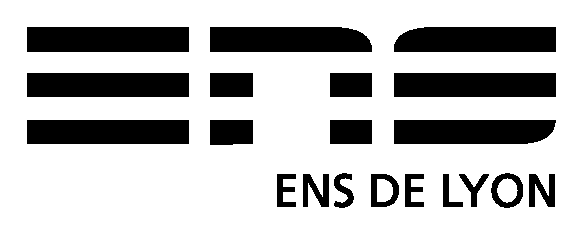
\includegraphics[scale=0.22]{logoens.eps}
\end{minipage}

\end{frame}
}

\section{What is active matter?}

\begin{frame}{Nonequilibrium systems}

Three general classes:\footfullcite{cates2015motility}
\begin{itemize}[<+->]
  \item Systems relaxing towards equilibrium.
  \item Systems with boundary conditions imposing steady currents.
  \item Active matter.
\end{itemize}

\only<1>{
\begin{example}
Thermal system adapting to its thermostat, glasses.
\end{example}
}
\only<2>{
\begin{example}
Sheared liquid, metal rod between two thermostats.
\end{example}
}

\end{frame}

\begin{frame}{Active matter}

\begin{definition}
System composed of self-driven units, \textit{active particles}, each capable of converting stored or ambient free energy into systematic movement.\footfullcite{marchetti2013hydrodynamics}
\end{definition}
\pause
\begin{example}
Cell tissues, swarms of bacteria, schools of fish, flocks of birds.
\end{example}

\end{frame}

\section{Model and method}

\subsection{Model}

\begin{frame}{Model system}

\blfootnote{\fullcite{fily2014freezing}}

\vspace{-0.5cm}
\begin{itemize}[<+->]
  \item 2D disks with packing fraction $\phi$ and 20\% polydispersity.
  \item Purely repulsive interparticle harmonic potential.
  \item Particle self-propulsion and Brownian dynamics.\\
\end{itemize}

\only<1>{}

\only<2>{
\vspace{-1cm}
\inserttikz{interparticle_interaction}{}

\vspace{-1cm}
\begin{align*}
\vec{F}_{ij} = \begin{cases} k(a_i + a_j - |\vec{r}_i - \vec{r}_j|) \hat{r}_{ij} &\text{if } a_i + a_j \geq |\vec{r}_i - \vec{r}_j| \\ 0 &\text{otherwise} \end{cases}
\end{align*}
}

\only<3>{
\vspace{-0.5cm}
\inserttikz{self_propulsion}{}

\vspace{-1cm}
\begin{align*}
\frac{d\vec{r}_i}{dt} &= \vec{v}_i + \sum_{j \neq i} \vec{F}_{ij} =  v_0\begin{pmatrix} \cos\theta_i \\ \sin\theta_i \end{pmatrix} + \sum_{j \neq i} \vec{F}_{ij}\\
\frac{d\theta_i}{dt} &= \eta_i(t) ~;~ \left<\eta_i(t)\eta_j(t^{\prime})\right> = 2 \nu_r \delta_{ij}\delta(t-t^{\prime})
\end{align*}
}

\only<4->{
\begin{itemize}
  \item[$\Rightarrow$] 3 control parameters:
  \only<5->{
  \begin{itemize}
    \item packing fraction $\phi$,
    \only<6->{\item dimensionless self-propulsion velocity $\tilde{v} = \frac{v_0}{ak}$,}
    \only<7->{\item and dimensionless rotation diffusion constant $\tilde{\nu}_r = \frac{\nu_r}{k}$ or equivalently dimensionless persistence time $\tau_r \equiv \tilde{\nu}_r^{-1}$.}
    \only<8>{\item[$\rightarrow$] P\'eclet number: $\text{Pe} = \frac{\tilde{v}}{\tilde{\nu}_r} \equiv$ dimensionless distance travelled before losing orientation.}
  \end{itemize}
  }
\end{itemize}
}

\end{frame}

\subsection{Method}

\begin{frame}{Simulation method}

\begin{itemize}
  \item[] Initialisation
  \begin{itemize}
    \item 20\% polydispersity
    \begin{itemize}
      \item[$\rightarrow$] mean radius $a$, 10 radii in the interval $[0.8a ; 1.2a]$
      \item[$\rightarrow$] uniform radii distribution
    \end{itemize}
    \item Particles intially randomly positioned
    \begin{itemize}
      \item[$\rightarrow$] then FIRE energy minimisation to decrease interpenetrations
    \end{itemize}
  \end{itemize}
  \item[] Integration
  \begin{itemize}
    \item Brownian integrator in \href{https://glotzerlab.engin.umich.edu/hoomd-blue/}{HOOMD-blue} simulation toolkit \faPython
  \end{itemize}
\end{itemize}

\end{frame}

\section{Observations}

\subsection{Motility-induced phase separation}

\begin{frame}{Spontaneous phase separation}

\insertmovie{0.7}{u_Dk5000_Vj1000_Rf5000_No2000_Il0000_Tl5000_Pl5000_Mn1000}{Spontaneous phase separation in our active system. $\vec{u}(t, t+\Delta t) \equiv$ particle displacement between times $t$ and $t+\Delta t$.}

\end{frame}

\begin{frame}{Motility-induced phase separation}

\blfootnote{\fullcite{cates2015motility}}

\only<1>{
\begin{definition}
Phase separated state arising in systems of motile particles which speed decreases sufficiently steeply with increasing local density.\\
A dilute active gas coexists with a dense liquid of substantially reduced motility.
\end{definition}
}

\only<2-9>{
\vspace{-0.5cm}
\inserttikz{mips}{Motility-induced phase separation mechanism diagram.}
}

\end{frame}

\begin{frame}{Phase diagram at fixed $\tilde{\nu}_r$}

\begin{figure}[h!]
  \centering
  \only<1>{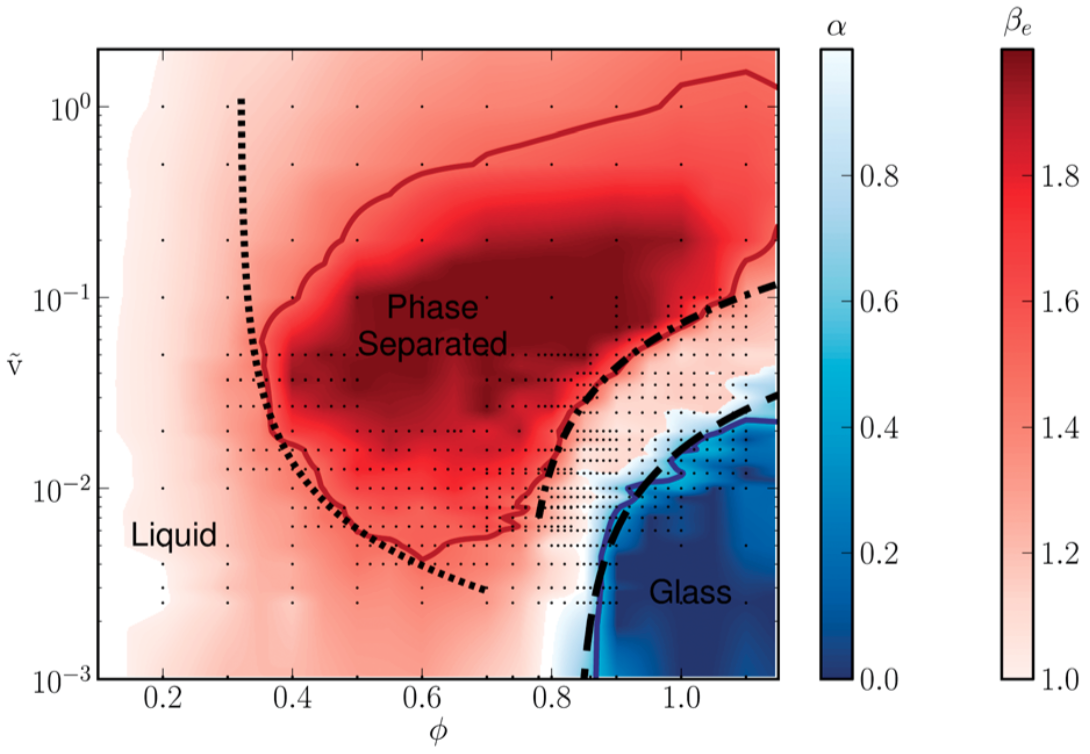
\includegraphics[width=0.7\linewidth]{phase_diagram.png}}
  \only<2>{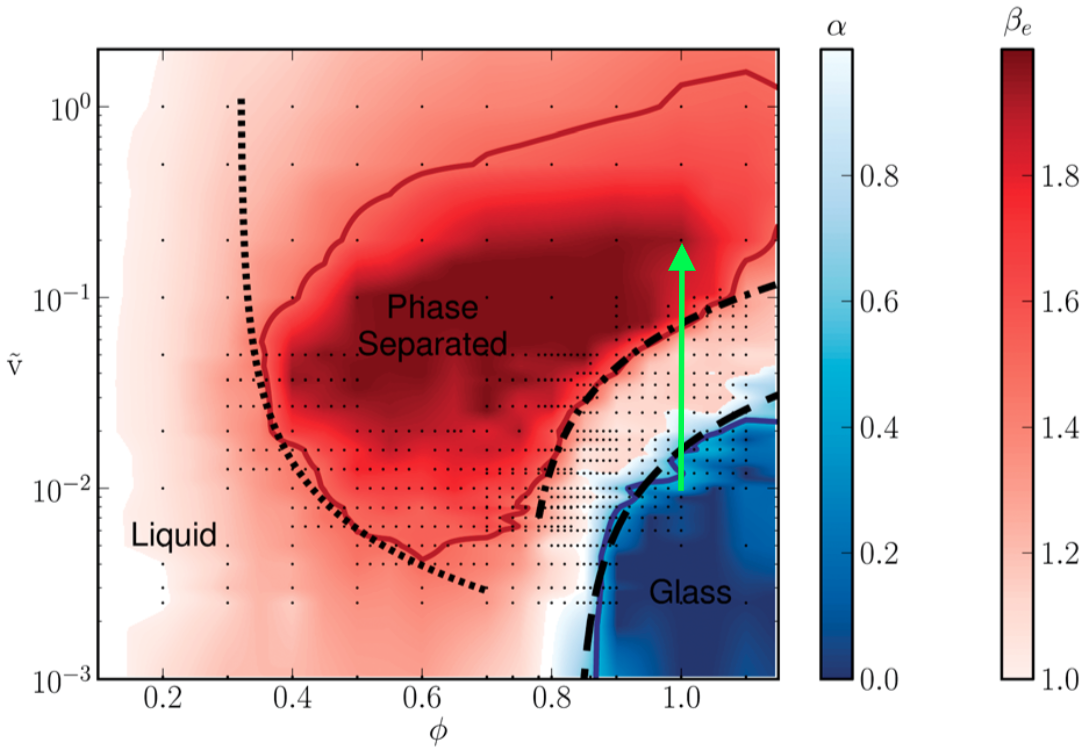
\includegraphics[width=0.7\linewidth]{phase_diagram_arrow.png}}
  \caption{Phase diagram for $\tilde{\nu}_r=5\cdot10^{-4}$.\footfullcite{fily2014freezing}}
\end{figure}

\end{frame}

\begin{frame}{Local density distribution with varying $\tilde{v}$}

\begin{figure}[h!]
  \centering
  \includegraphics[width=0.9\linewidth]{Pphiloc_Dl1000_Rh3000_Nq1000_Io5000_Ml1000_Cn5000.eps}
  \caption{Histogram of local density $\phi_{loc}$ with varying self-propulsion velocity $\tilde{v}$, at packing fraction $\phi=1.00$ and rotation diffusion constant $\tilde{\nu}_r = 3\cdot10^{-4}$.}
\end{figure}

\end{frame}

\begin{frame}{Phase diagram boundaries with varying $\tilde{\nu}_r$}

\begin{figure}[h!]
  \centering
  \only<1>{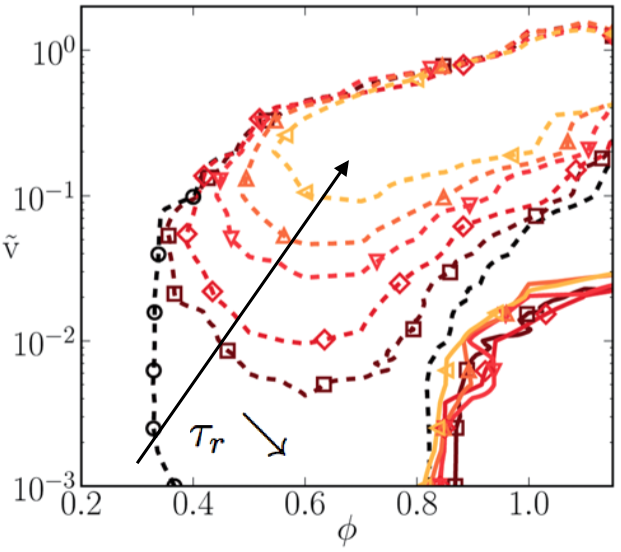
\includegraphics[width=0.5\linewidth]{phase_boundary.png}}
  \only<2>{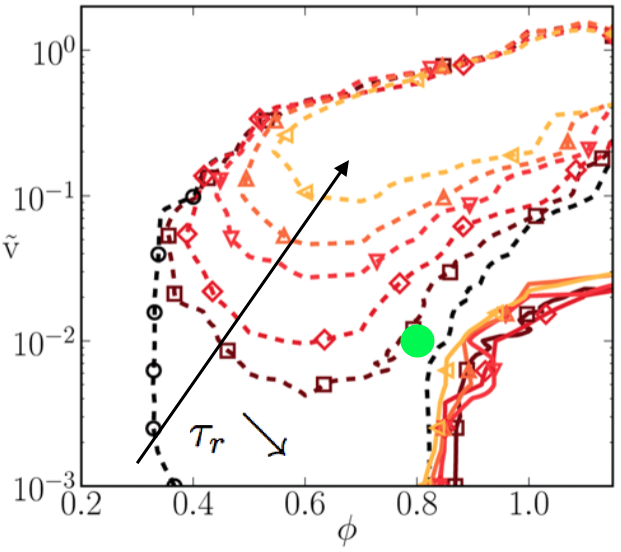
\includegraphics[width=0.5\linewidth]{phase_boundary_dot.png}}
  \caption{Boundaries of glassy (solid lines) and phase separated (dashed lines) regions for different persistence times $\tau_r$.\footfullcite{fily2014freezing}}
\end{figure}

\end{frame}

\begin{frame}{Local density distribution with varying $\tilde{\nu}_r$}

\begin{figure}[h!]
  \centering
  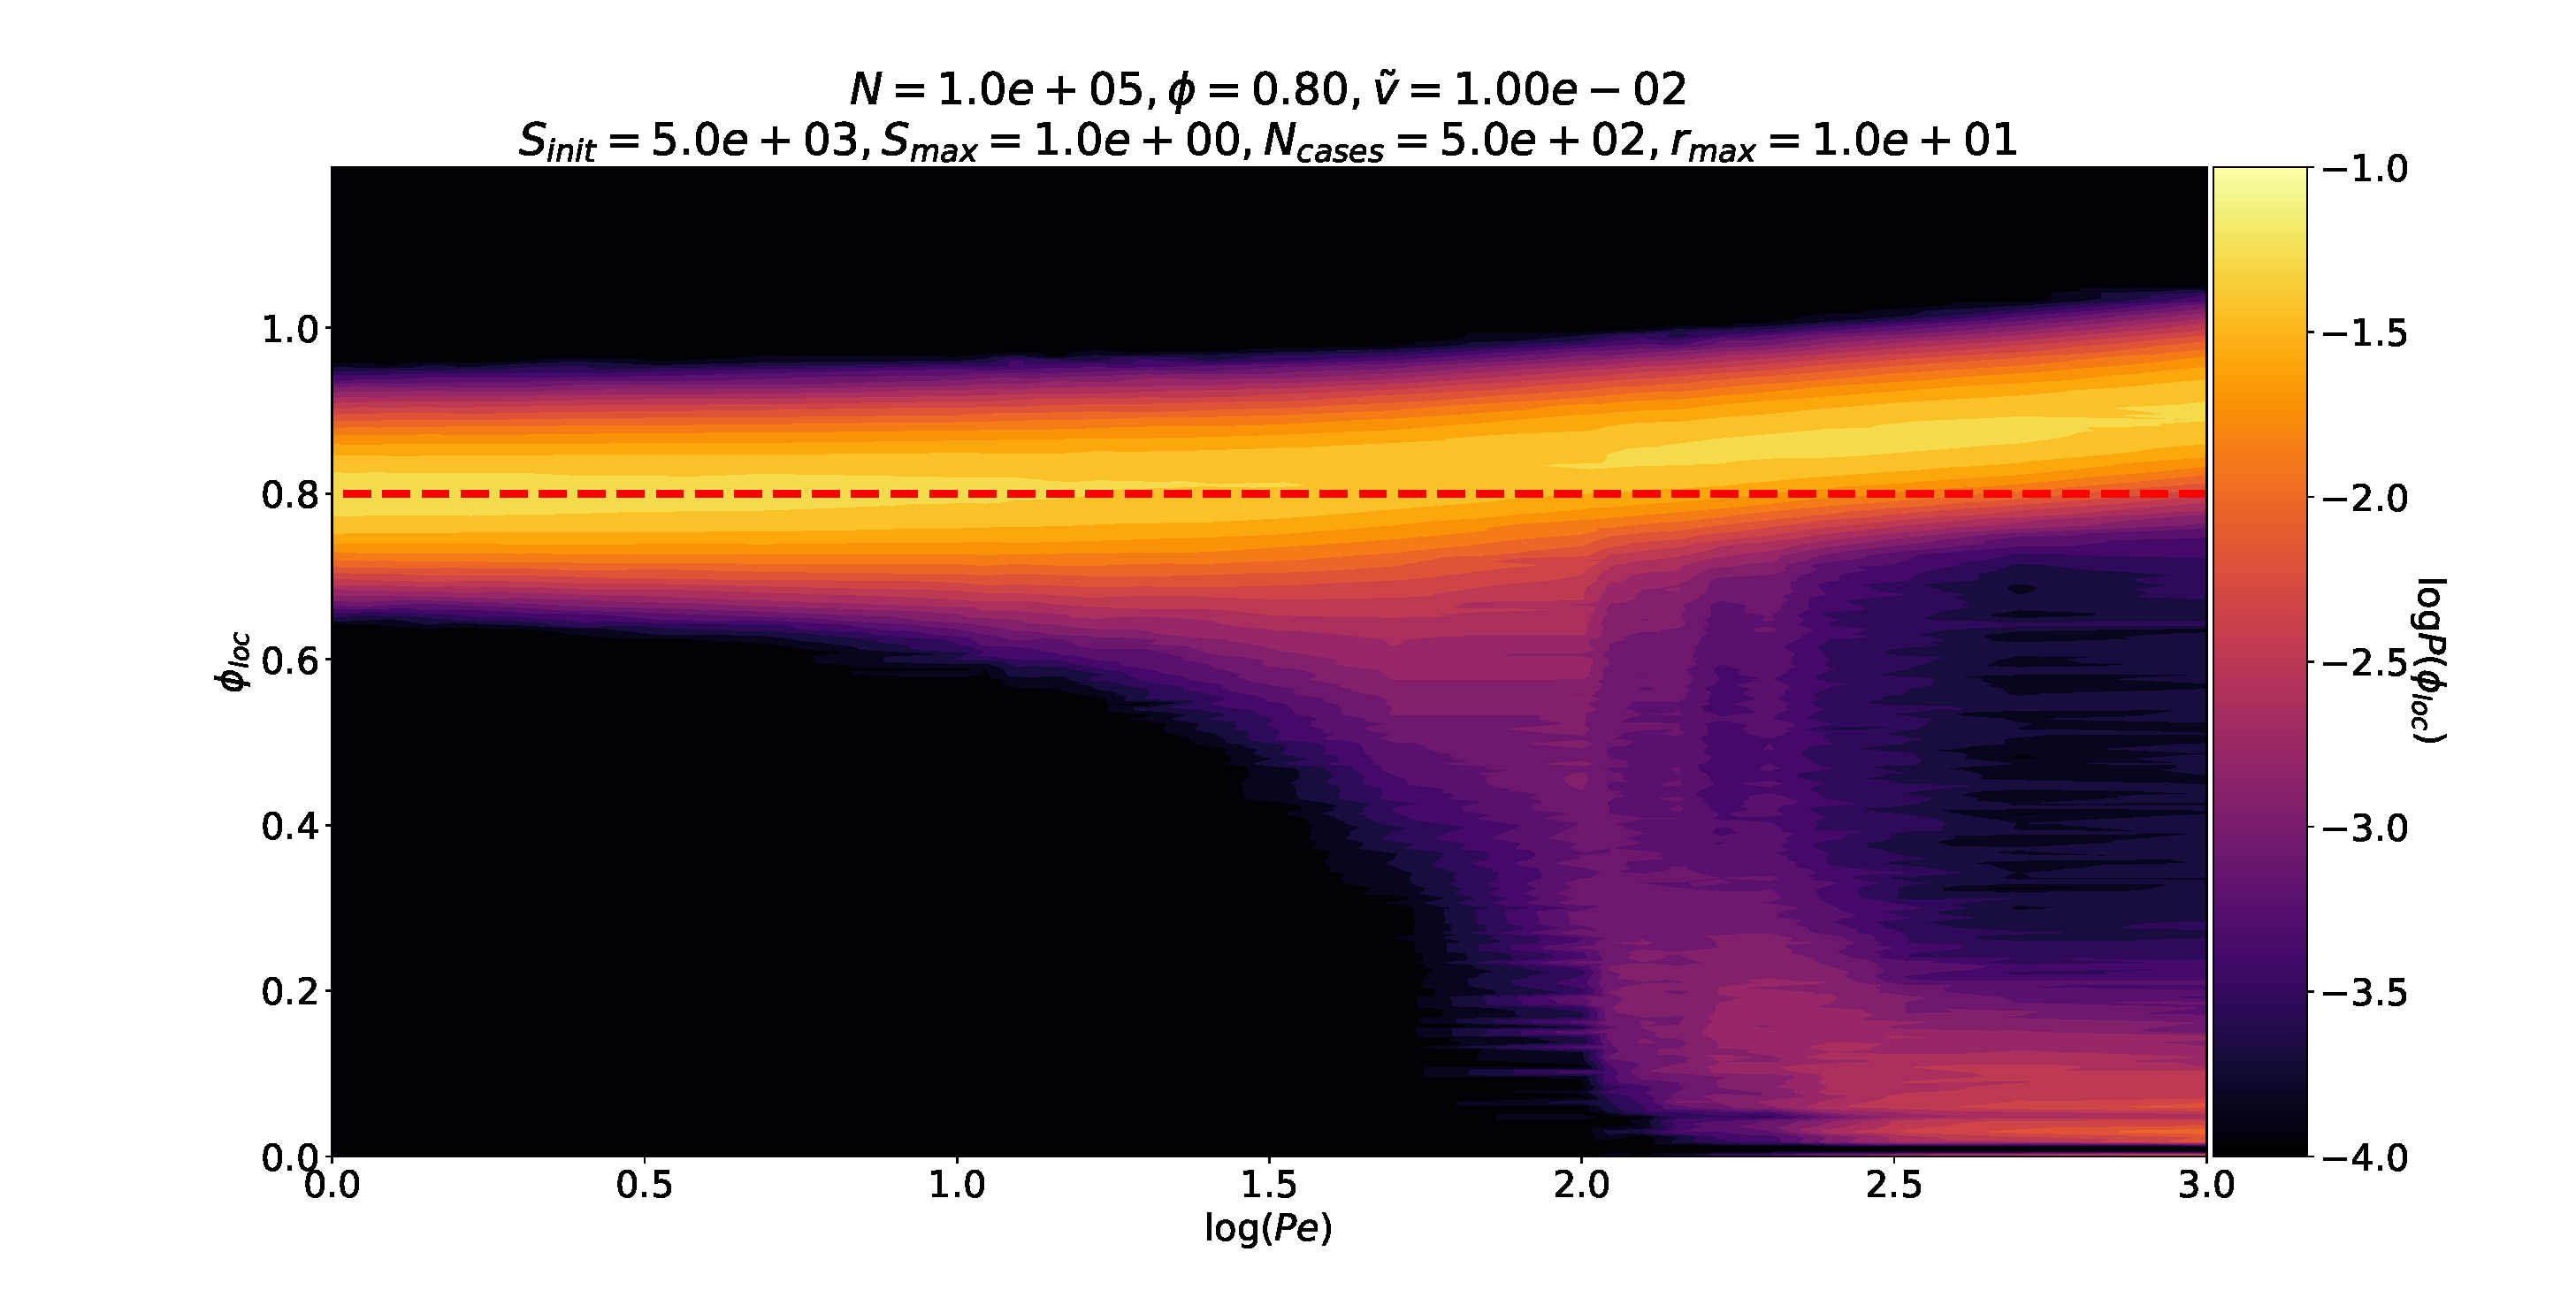
\includegraphics[width=0.9\linewidth]{Pphiloc_Dk8000_Vj1000_Nq1000_Io5000_Ml1000_Cn5000.eps}
  \caption{Histogram of local density $\phi_{loc}$ with varying rotation diffusion constant $\tilde{\nu}_r$, at packing fraction $\phi=0.80$ and rotation diffusion constant $\tilde{v} = 1\cdot10^{—2}$.}
\end{figure}

\end{frame}

\subsection{Displacement correlations and cooperativities}

\begin{frame}{Displacement map at low activity}

\vspace{-0.25cm}
\insertmovie{0.7}{u_Dk8000_Vj1000_Rj1000_Nq1000_Io5000_Tm1000_Bn1000_Pl1000_Mm5000}{Displacement maps at low activity ($\tilde{\nu}_r = 1\cdot10^{-2}$) with $\tilde{\nu}_r\Delta t = 1$. $\vec{u}(t, t+\Delta t) \equiv$ particle displacement between times $t$ and $t+\Delta t$.}

\end{frame}

\begin{frame}{Displacement map at high activity}

\vspace{-0.25cm}
\insertmovie{0.7}{u_Dk8000_Vj1000_Rg2000_Nq1000_Io5000_Tm5000_Bn1000_Pl5000_Mm5000}{Displacement maps at high activity ($\tilde{\nu}_r = 2\cdot10^{-5}$) with $\tilde{\nu}_r\Delta t = 1$. $\vec{u}(t, t+\Delta t) \equiv$ particle displacement between times $t$ and $t+\Delta t$.}

\end{frame}

\begin{frame}{Displacement correlation}

$\vec{u}(\vec{r}, t, t + \Delta t) \equiv$ displacement of particle at position $\vec{r}$ between times $t$ and $t + \Delta t$

\begin{align*}
C_{uu}(\Delta \vec{r}, \Delta t) &= \left<\vec{u}(\vec{r}+\Delta\vec{r}, t, t + \Delta t)\cdot\vec{u}(\vec{r}, t, t + \Delta t)\right>
\only<2->{
\\
&= \frac{\int dt \int d^2\vec{r}~ \vec{u}(\vec{r}, t, t+\Delta t)\cdot\vec{u}(\vec{r} + \Delta \vec{r}, t, t+\Delta t)}{\int dt \int d^2\vec{r}~ ||\vec{u}(\vec{r}, t, t+\Delta t)||^2}
}
\only<3->{
\\
&= \frac{\mathcal{F}^{-1}\{\int dt~ ||\mathcal{F}\{\vec{u}\}(\vec{k}, t, t + \Delta t)||^2\}(\Delta \vec{r}, \Delta t)}{\int dt \int d^2\vec{r}~ ||\vec{u}(\vec{r}, t, t+\Delta t)||^2}
}
\end{align*}
\only<4>{
\begin{align*}
C_{uu}(\Delta \vec{r}, \Delta t) \xrightarrow[\text{isotropy}]{} C_{uu}(\Delta r, \Delta t)
\end{align*}
}

\end{frame}

\begin{frame}{Necessity of dividing by density correlation}

\only<1-4>{
Displacements are put on a grid to calculate their correlations.
\begin{align*}
\vec{u}(\vec{r}_i, t, t + \Delta t) \xrightarrow[\substack{\text{coarse-graining}\\\text{(average in grid box)}}]{} \vec{u}_{ij}(t, t + \Delta t) \only<2-4>{\xrightarrow[\text{FFT}]{} C_{uu, ij}}
\end{align*}
}

\only<3-4>{
\textbf{Issue:} small grid spacing $\Rightarrow$ significant amount of grid boxes are empty.
}

\only<4>{
\begin{align*}
\rho_{ij} = \begin{cases} 1 &\text{ if } \vec{u}_{ij} \neq \vec{0} \\ 0 &\text{ otherwise} \end{cases} \equiv \text{density}
\end{align*}
Small grid spacing $\Rightarrow$ significant amount of $\rho_{ij}$ are equal to 0.
}

\only<5>{
\vspace{-0.5cm}
\begin{figure}[h!]
  \centering
  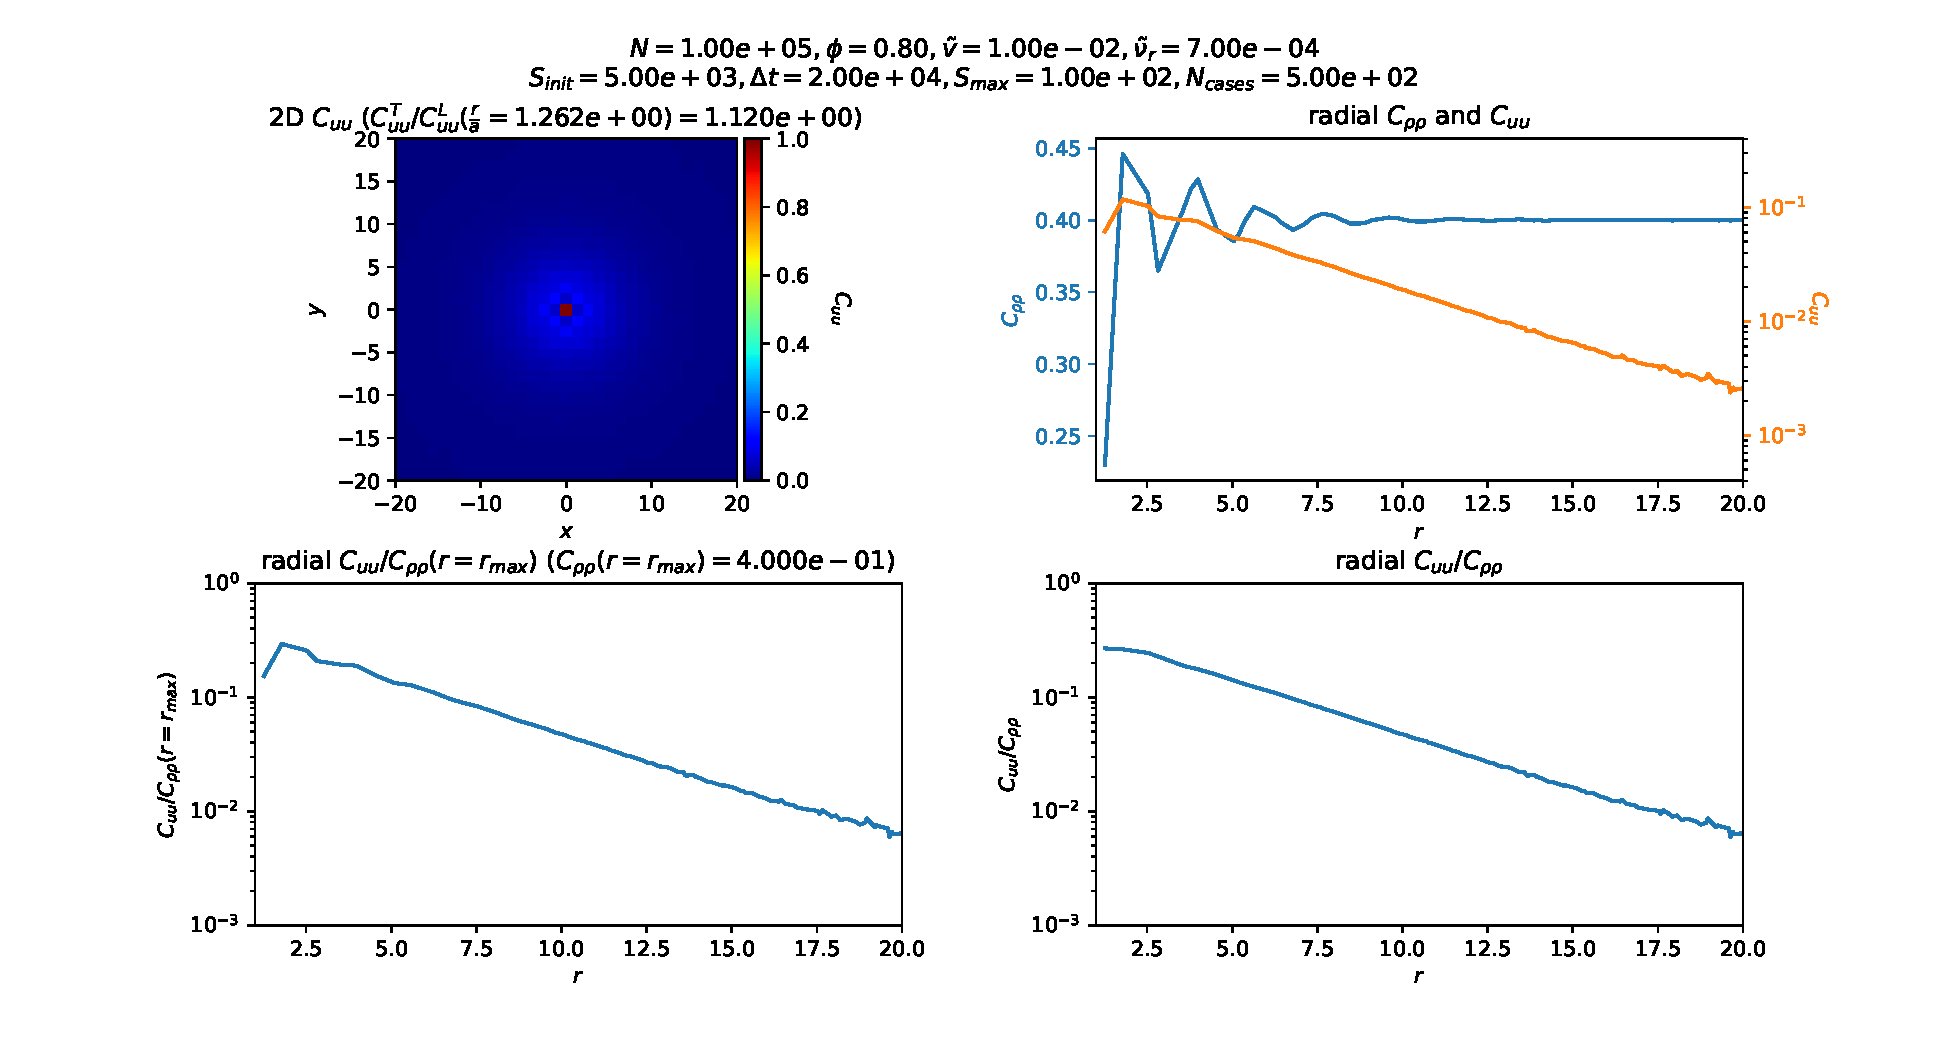
\includegraphics[width=0.9\linewidth]{Cuub_Dk8000_Vj1000_Rh7000_Nq1000_Io5000_Tn2000_Mn1000_Cn5000_LINLOG.eps}
  \caption{Displacement correlations $C_{uu}(r, \Delta t)$ and density correlations $C_{\rho\rho}(r)$, at packing fraction $\phi=0.80$, self-propulsion velocity $\tilde{v}=1\cdot10^{-2}$, and rotation diffusion constant $\tilde{\nu}_r = 7\cdot10^{-4}$.}
\end{figure}
\vspace{-0.5cm}
$\rightarrow C_{uu,ij}$ has to be divided by $C_{\rho\rho, ij} \propto$ radial distribution function.
}

\end{frame}

\begin{frame}{Displacement correlation}

\begin{figure}[h!]
  \centering
  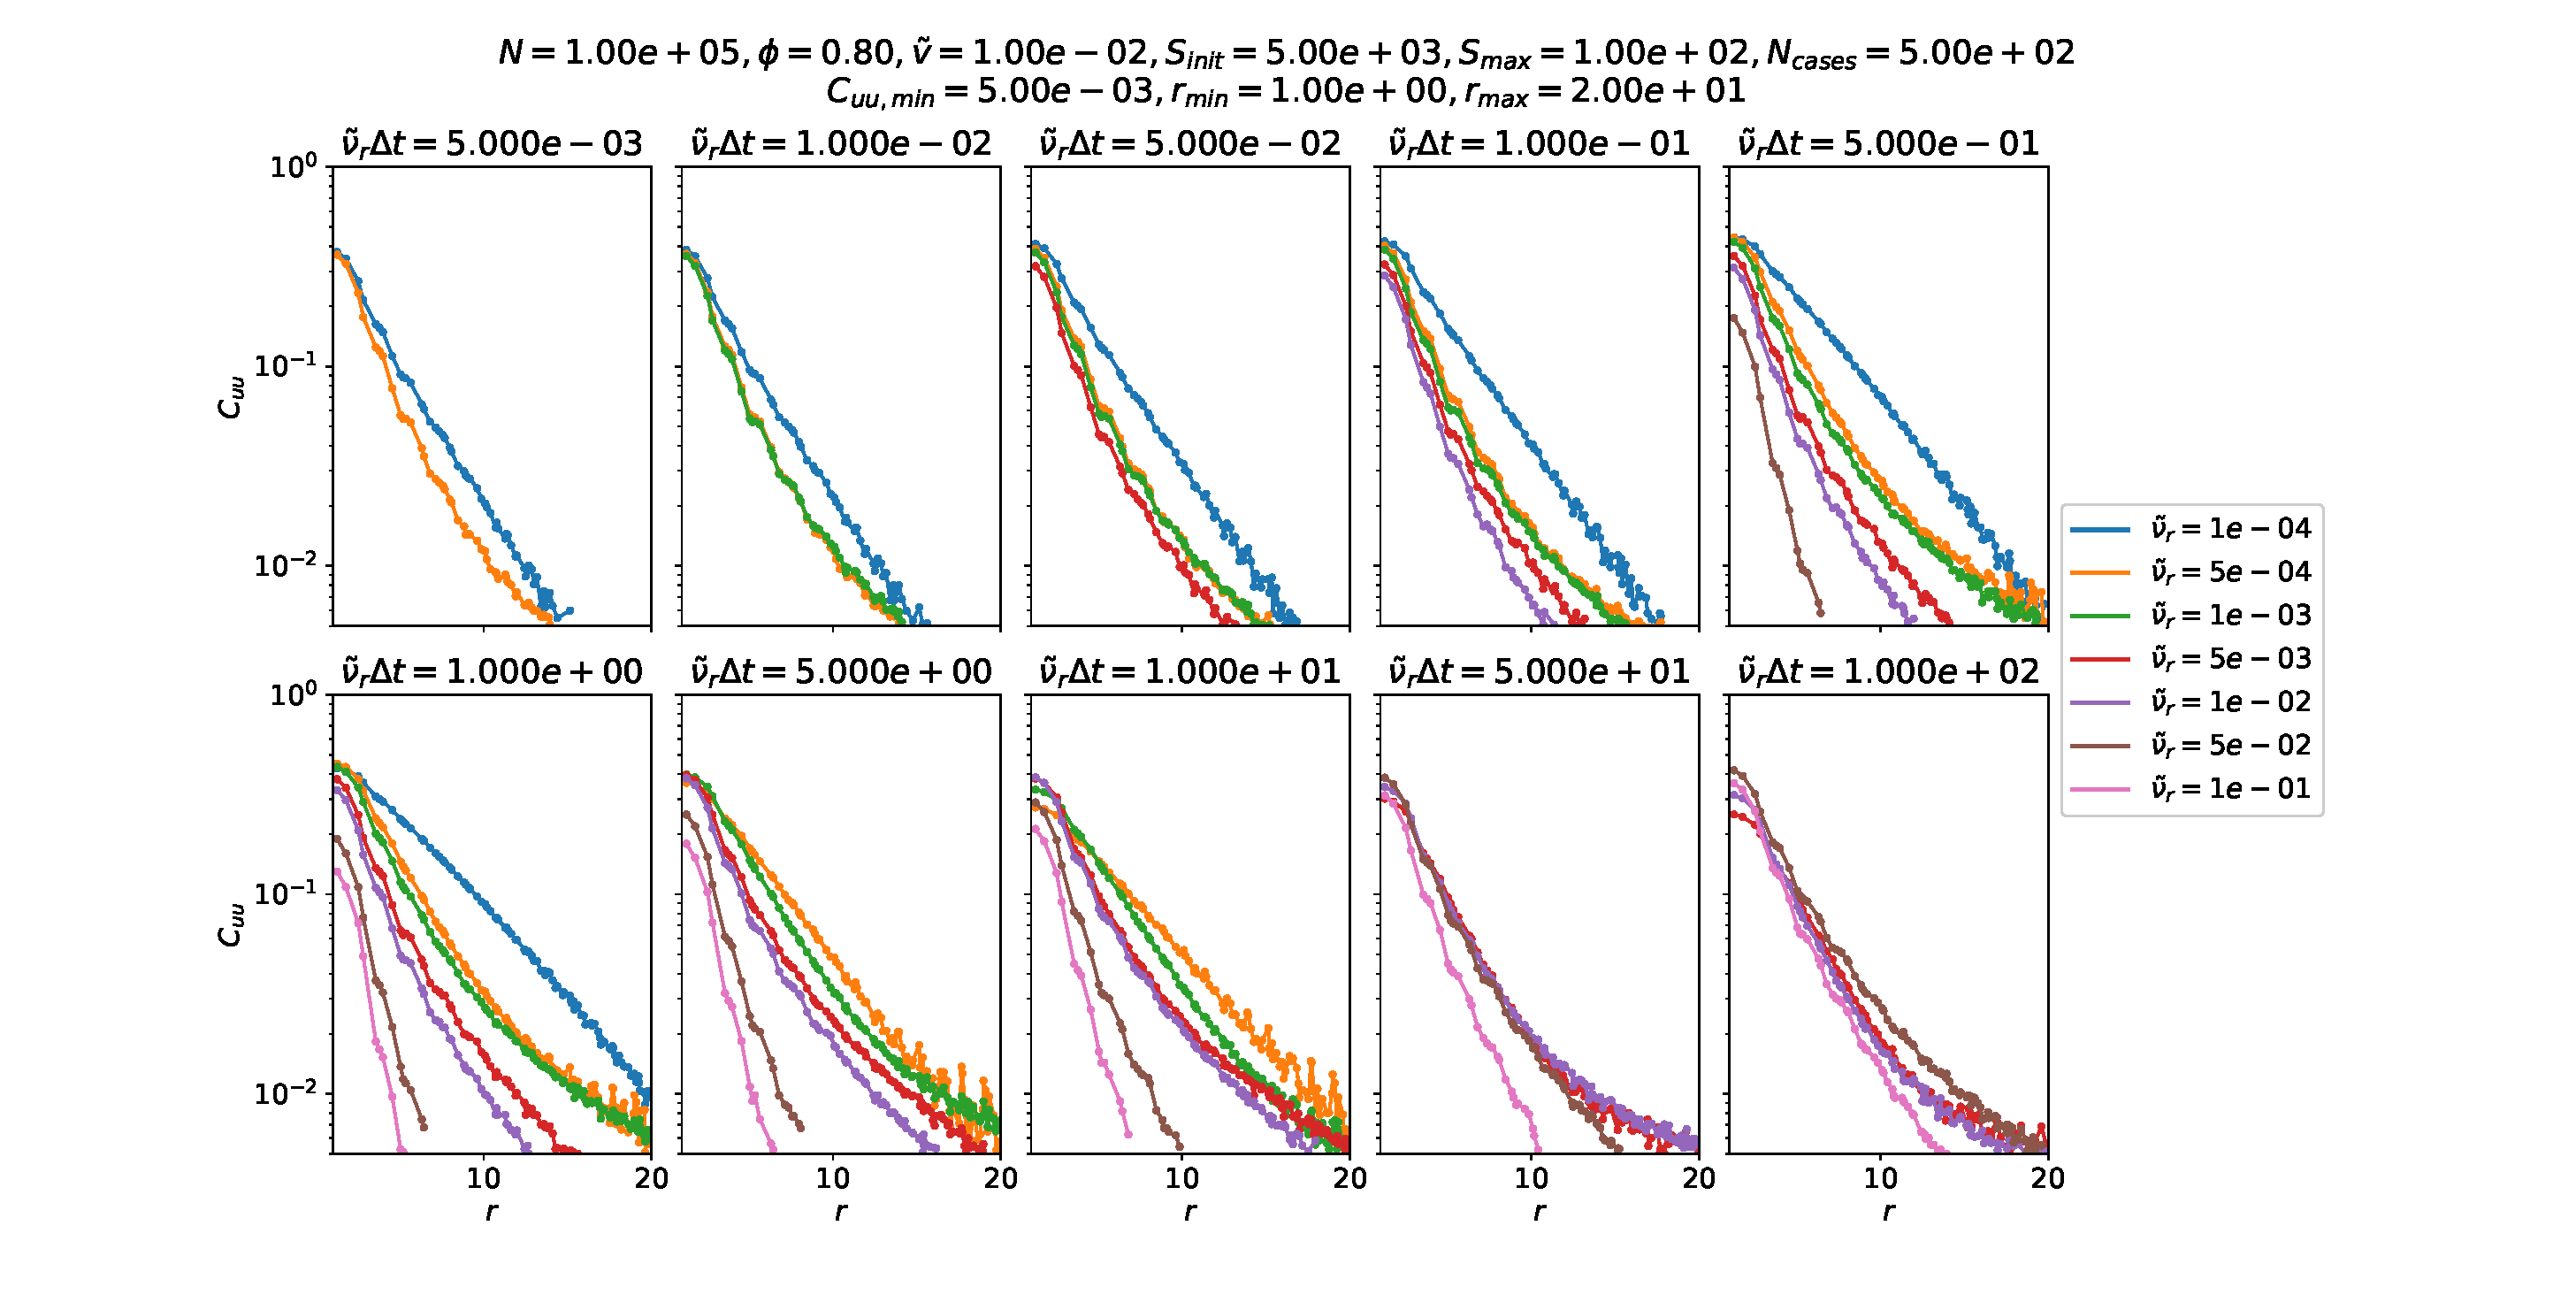
\includegraphics[width=\linewidth]{Cuu_comparison_Dk8000_Vj1000_Nq1000_Cn5000_LINLOG.eps}
  \caption{Comparison of displacement correlations $C_{uu}(r, \Delta t)$ for equal numbers of rotations $\tilde{\nu}_r\Delta t$, at packing fraction $\phi=0.80$ and self-propulsion velocity $\tilde{v}=1\cdot10^{-2}$.}
\end{figure}

\end{frame}

\begin{frame}{Displacement cooperativity}

\blfootnote{\fullcite{wysocki2014cooperative}}
\blfootnote{\fullcite{doliwa2000cooperativity}}

\begin{align*}
\chi(\Delta t, r_{min}, r_{max}) = \frac{1}{L^2} \int_{r=r_{min}}^{r=r_{max}}  dr~ 2\pi r~ C_{uu}(r, \Delta t)
\end{align*}
with $L$ the characteristic length of the system.\\

\begin{definition}
$\chi \equiv$ average proportion of particles acting as coherently moving neighbours $\rightarrow$ measure of dynamical heterogeneity.
\end{definition}

\end{frame}

\begin{frame}{Displacement cooperativity with varying $\tilde{\nu}_r$}

%\vspace{-0.5cm}
\begin{figure}[h!]
  \centering
  \only<1>{
  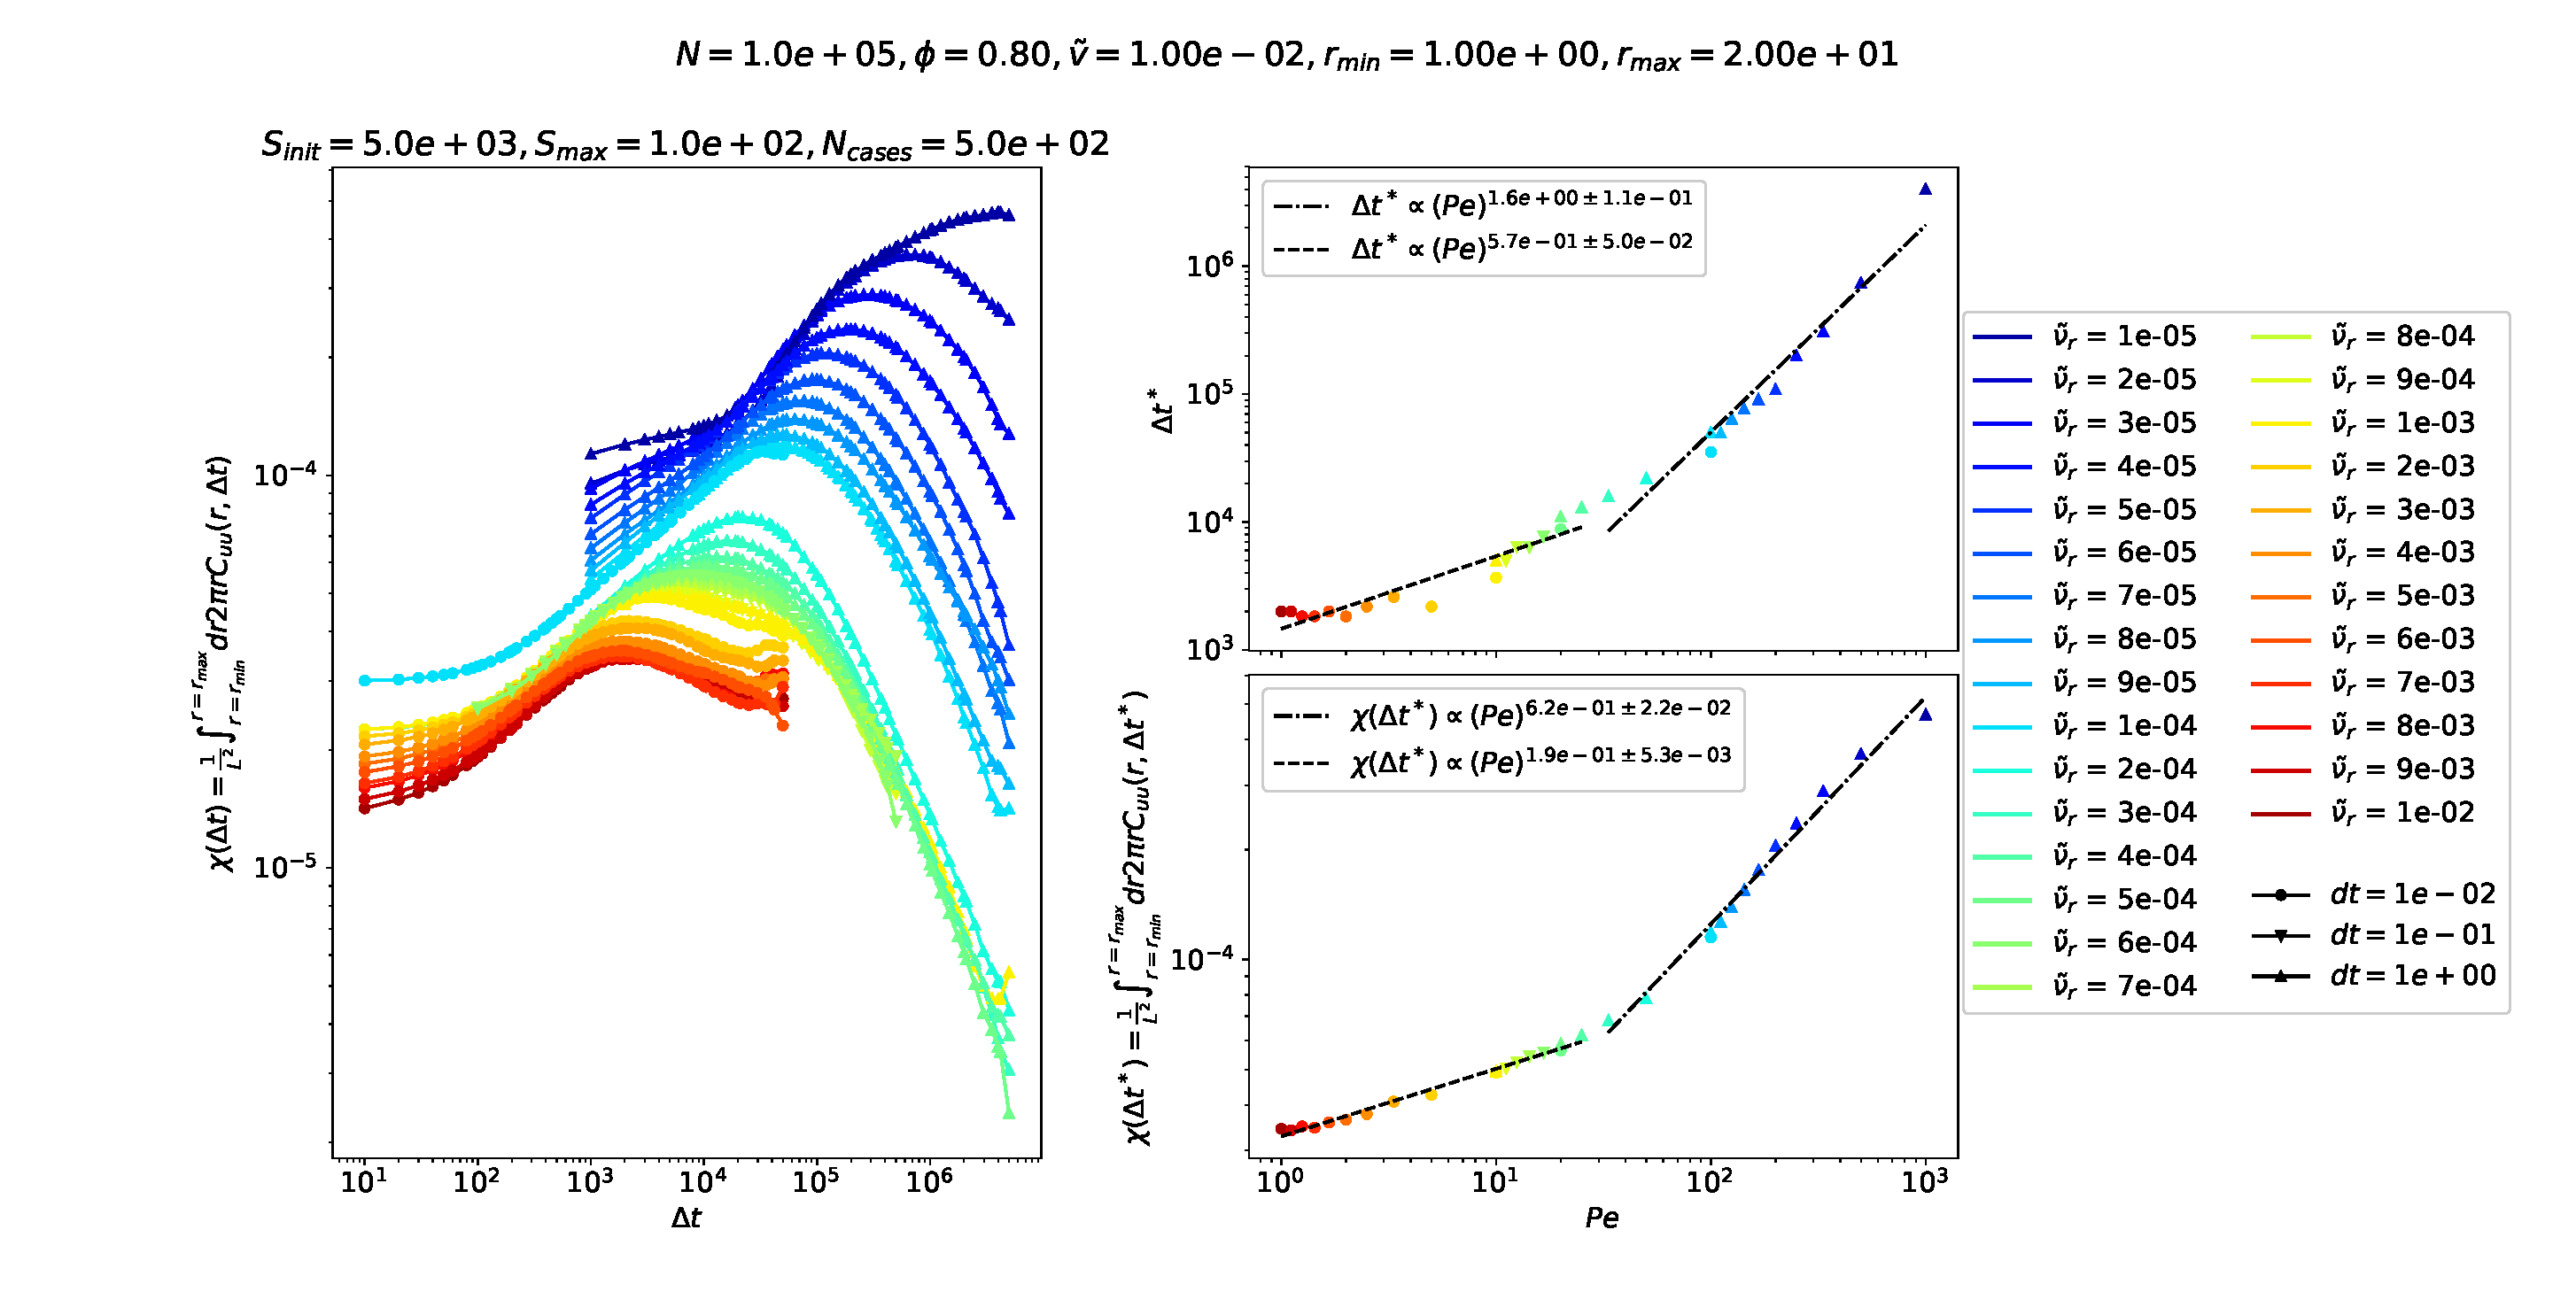
\includegraphics[width=0.9\linewidth]{intCuu_dt_Dk8000_Vj1000_Nq1000_Io5000_Mn1000_Cn5000_RMINl1000_RMAXm2000.eps}
  \vspace{-0.3cm}
  \caption{Comparison of displacement cooperativities $\chi(\Delta t)$, times of maximum cooperativity $\Delta t^*$ and maximum cooperativities $\chi(\Delta t^*)$, at packing fraction $\phi=0.80$ and self-propulsion velocity $\tilde{v}=1\cdot10^{-2}$.}
  }
  \only<2>{
  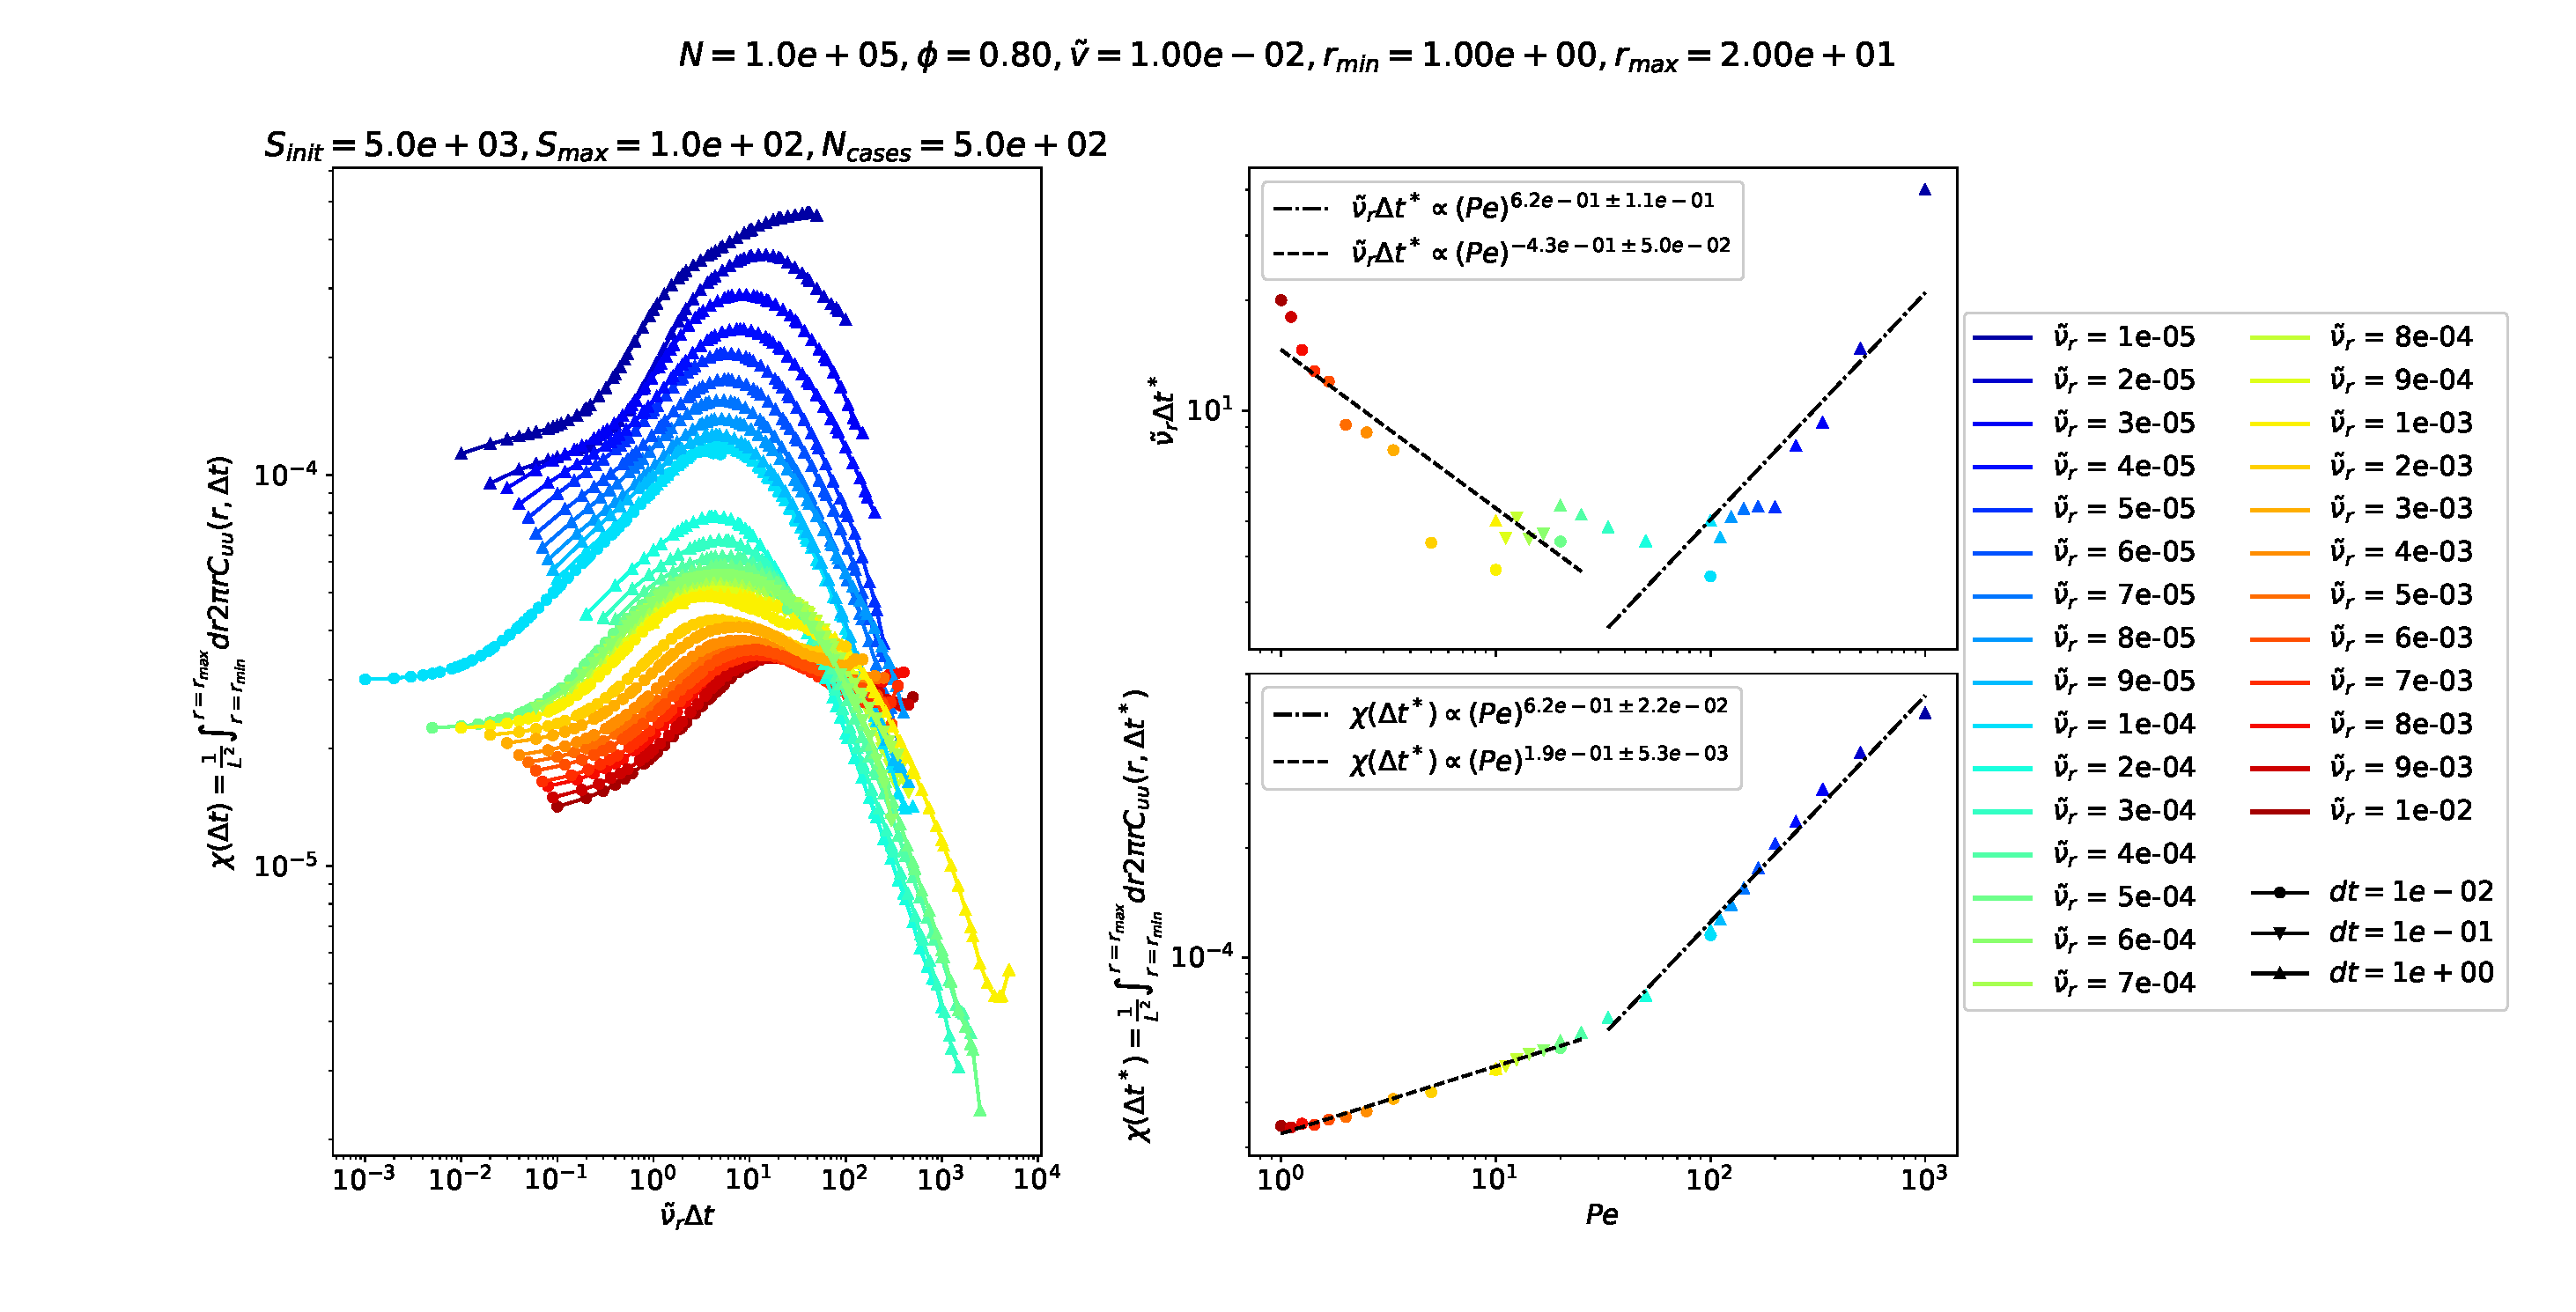
\includegraphics[width=0.9\linewidth]{intCuu_Dk8000_Vj1000_Nq1000_Io5000_Mn1000_Cn5000_RMINl1000_RMAXm2000.eps}
  \vspace{-0.3cm}
  \caption{Comparison of displacement cooperativities $\chi(\Delta t)$, number of rotations of maximum cooperativity $\tilde{\nu}_r\Delta t^*$ and maximum cooperativities $\chi(\Delta t^*)$, at packing fraction $\phi=0.80$ and self-propulsion velocity $\tilde{v}=1\cdot10^{-2}$.}
  }
\end{figure}

\vspace{-0.5cm}
\only<1>{
\begin{itemize}
  \item[$\rightarrow$] Clear change of $\Delta t^*(\text{Pe})$ and $\chi(\Delta t^*, \text{Pe})$ slopes at MIPS.
  \item[$\rightarrow$] $(\tau_r \nearrow~ \Leftrightarrow \text{Pe} \nearrow) \Rightarrow \Delta t^* \nearrow,~ \chi(\Delta t^*)\nearrow$
\end{itemize}
}
\only<2>{
\begin{itemize}
  \item[$\rightarrow$] Clear change of $\tilde{\nu}_r\Delta t^*(\text{Pe})$ and $\chi(\Delta t^*, \text{Pe})$ slopes at MIPS.
  \item[$\rightarrow$] Non-monotonous variations of $\tilde{\nu}_r\Delta t^*$ with $\text{Pe}$.
\end{itemize}
}

\end{frame}

\begin{frame}{Ageing effect with varying $\tilde{\nu}_r$}

\vspace{-0.2cm}
\begin{figure}[h!]
  \centering
  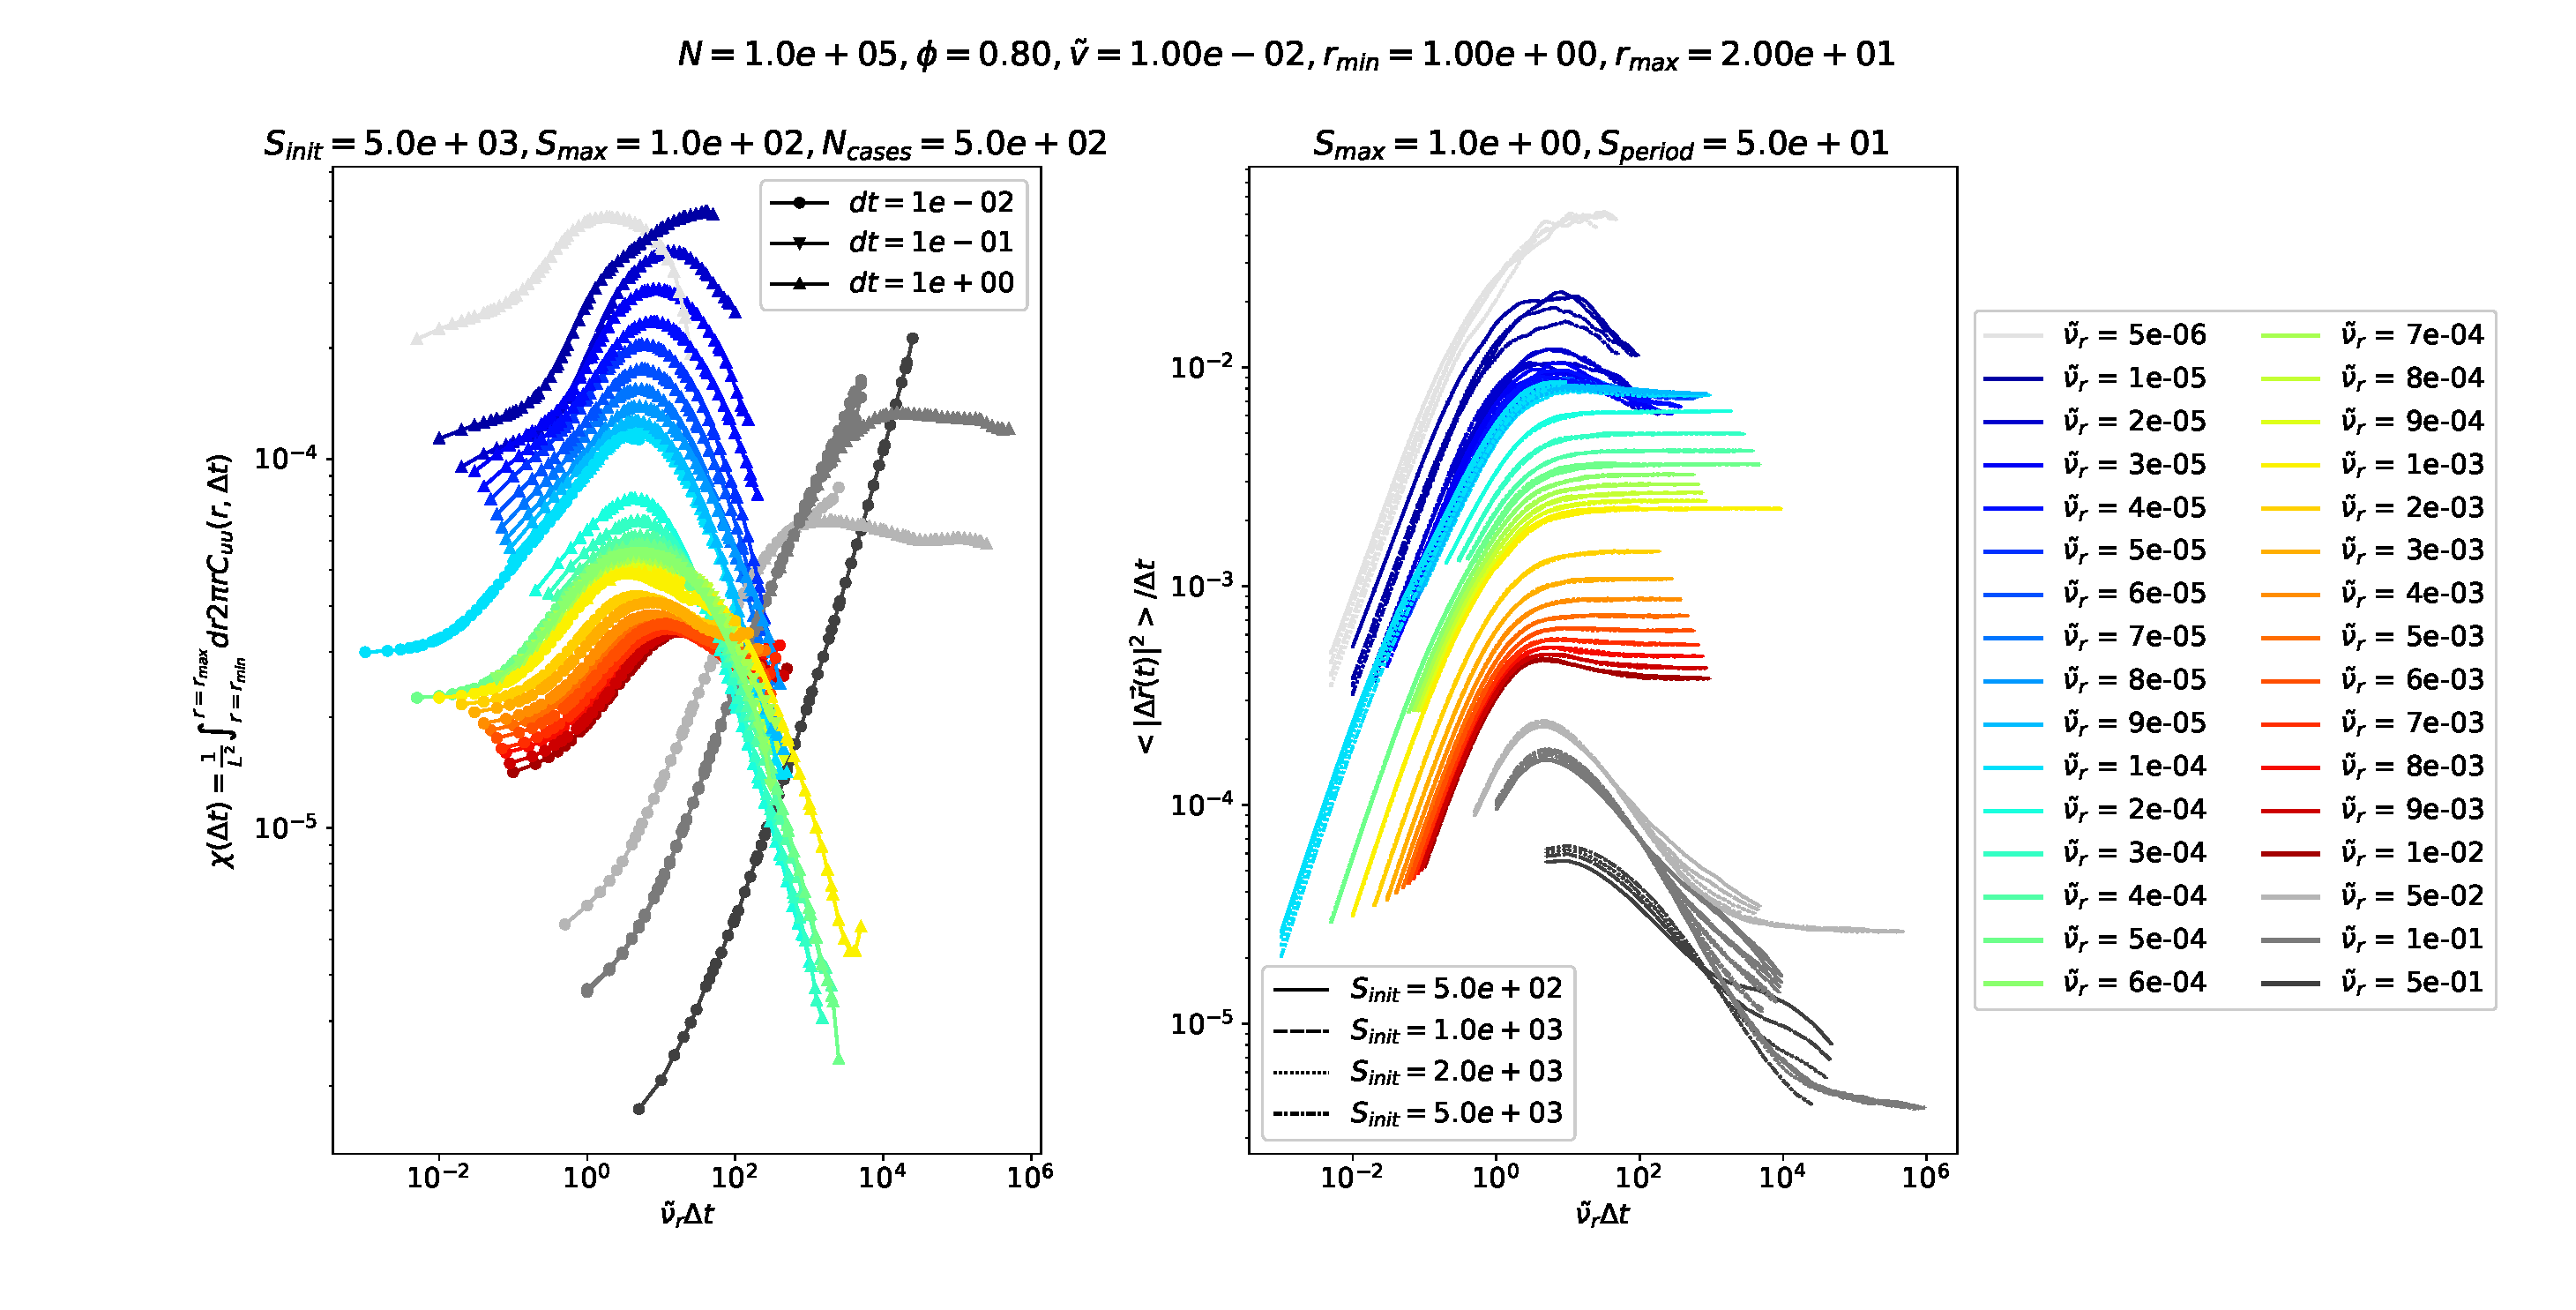
\includegraphics[width=0.8\linewidth]{intCuu_msdt_Dk8000_Vj1000_Nq1000_Io5000_Mn1000_Cn5000_RMINl1000_RMAXm2000.eps}
  \vspace{-0.2cm}
  \caption{Comparison of displacement cooperativities $\chi(\Delta t)$ and mean square displacements divided by lag times $<|\Delta\vec{r}(\Delta t)|^2>/\Delta t$, at packing fraction $\phi=0.80$ and self-propulsion velocity $\tilde{v}=1\cdot10^{-2}$.}
\end{figure}
\vspace{-0.3cm}
Subdiffusive behaviour and ageing effect characteristic of glassiness
\begin{itemize}
  \item[$\rightarrow$] at high activity (phase-separated regime),
  \item[$\rightarrow$] at very low activity (glass phase).
\end{itemize}

\end{frame}

\begin{frame}{Displacement cooperativity with varying $\tilde{v}$}

\vspace{-0.2cm}
\begin{figure}[h!]
  \centering
  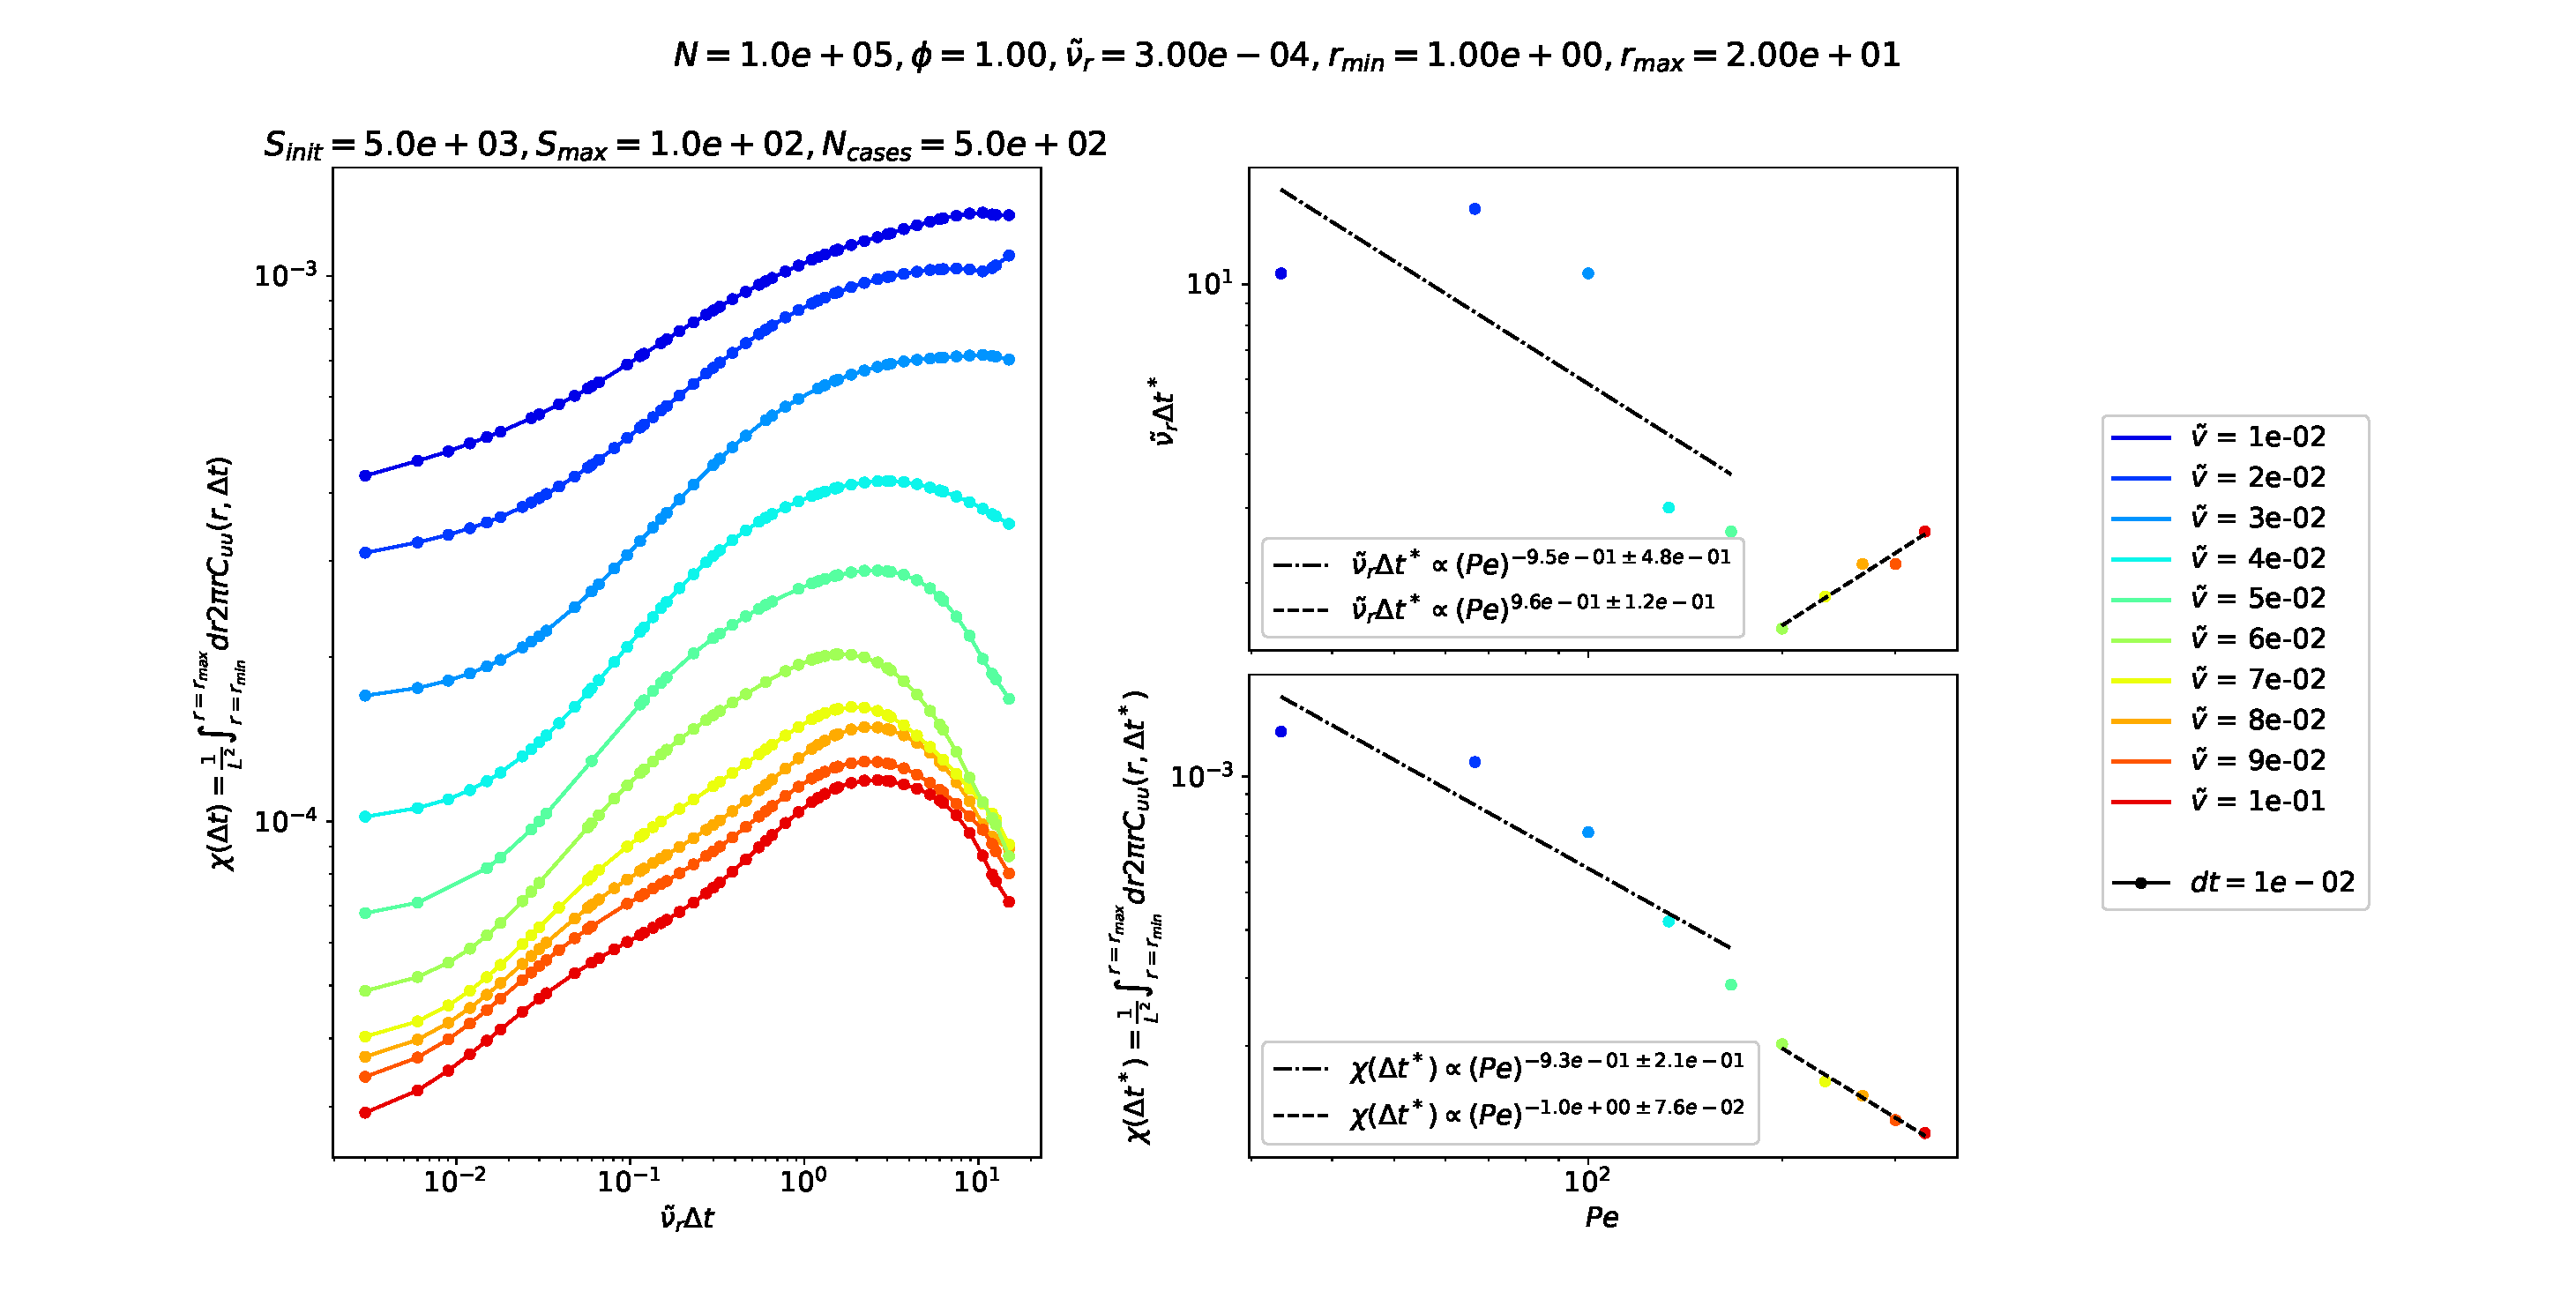
\includegraphics[width=0.8\linewidth]{intCuu_Dk8000_Rh3000_Nq1000_Io5000_Mn1000_Cn5000_RMINl1000_RMAXm2000.eps}
  \vspace{-0.2cm}
  \caption{Comparison of displacement cooperativities $\chi(\Delta t)$, number of rotations of maximum cooperativity $\tilde{\nu}_r\Delta t^*$ and maximum cooperativities $\chi(\Delta t^*)$, at packing fraction $\phi=1.00$ and self-propulsion velocity $\tilde{\nu}_r=3\cdot10^{-4}$.}
\end{figure}

\vspace{-0.3cm}
\begin{itemize}
  \item[$\rightarrow$] Change of $\tilde{\nu}_r \Delta t^*(\text{Pe})$ and $\chi(\Delta t^*, \text{Pe})$ slopes at MIPS.
  \item[$\rightarrow$] $(\tilde{v} \searrow~ \Leftrightarrow \text{Pe} \nearrow) \Rightarrow \chi(\Delta t^*)\searrow$
  \item[$\rightarrow$] Non-monotonous variations of $\tilde{\nu}_r\Delta t^*$ with $\text{Pe}$.
\end{itemize}

\end{frame}

\begin{frame}{Ageing effect with varying $\tilde{v}$}

\vspace{-0.2cm}
\begin{figure}[h!]
  \centering
  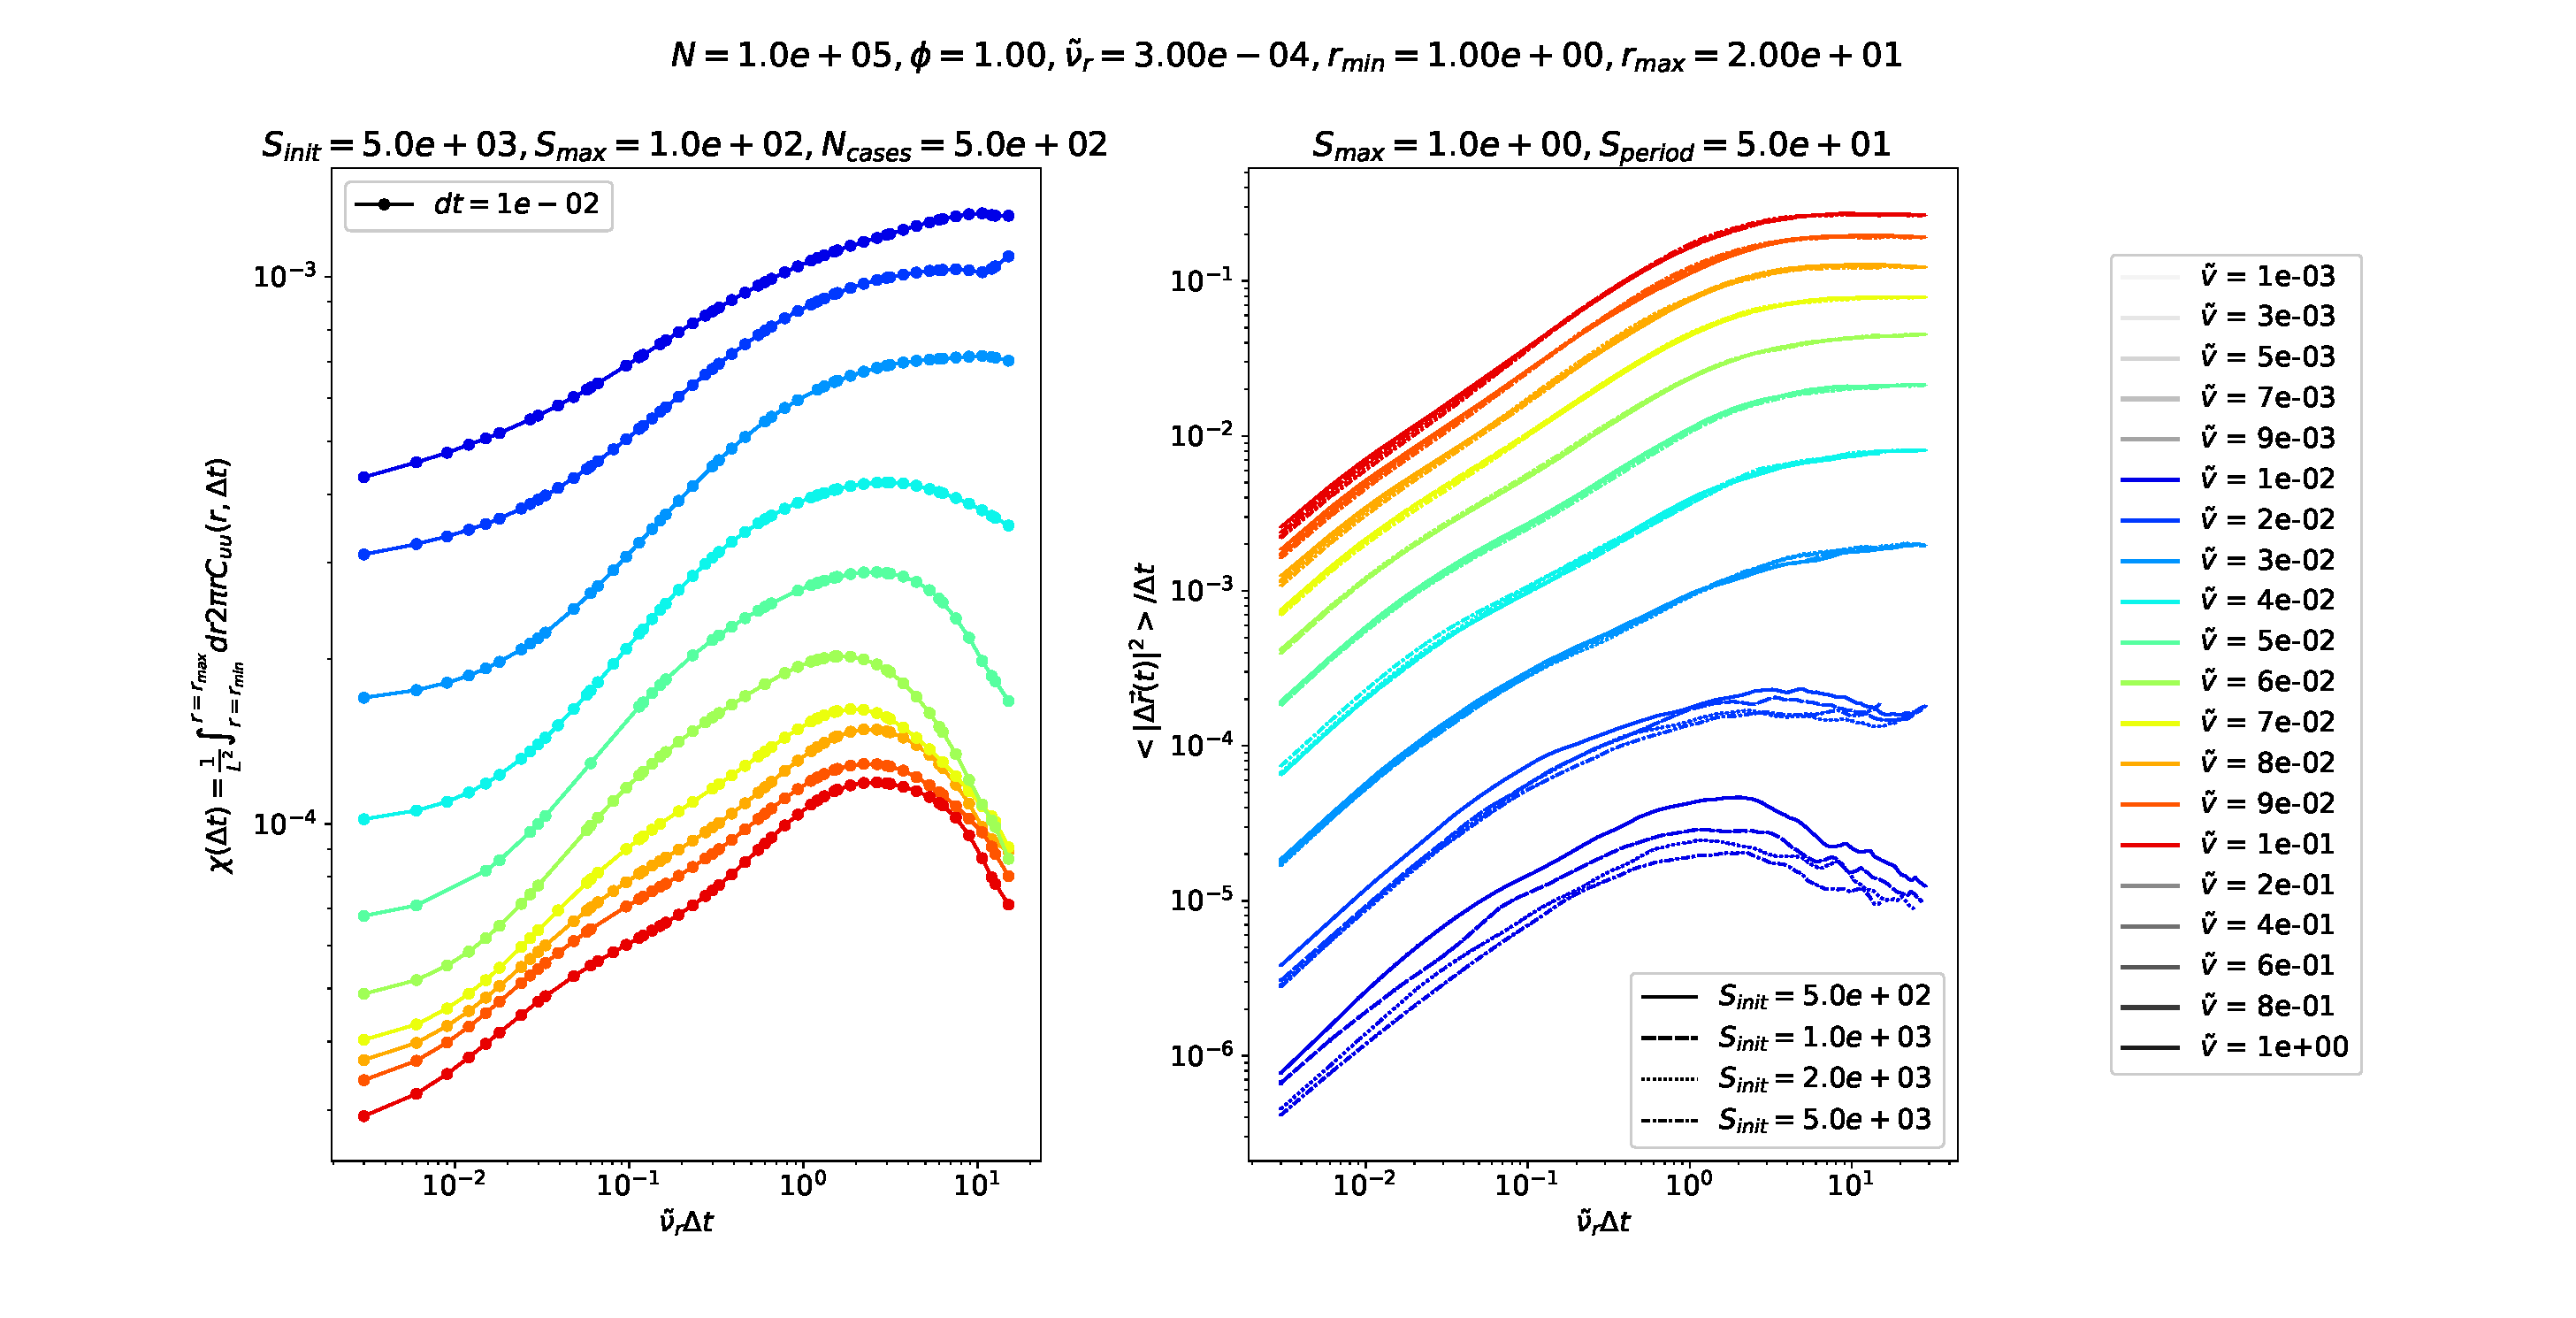
\includegraphics[width=0.8\linewidth]{intCuu_msdt_Dk8000_Rh3000_Nq1000_Io5000_Mn1000_Cn5000_RMINl1000_RMAXm2000.eps}
  \vspace{-0.2cm}
  \caption{Comparison of displacement cooperativities $\chi(\Delta t)$ and mean square displacements divided by lag times $<|\Delta\vec{r}(\Delta t)|^2>/\Delta t$, at packing fraction $\phi=1.00$ and rotation diffusion constant $\tilde{\nu}_r=3\cdot10^{-4}$.}
\end{figure}
\vspace{-0.3cm}
Subdiffusive behaviour and ageing effect characteristic of glassiness at low self-propulsion velocity (glass phase).

\end{frame}

\begin{frame}{Directional displacement correlations}

\blfootnote{\fullcite{weeks2007short}}
\blfootnote{\fullcite{vasisht2018rate}}

\vspace{-1cm}
\begin{align*}
\vec{u}(\vec{r}, t, t + \Delta t) &= \overbrace{\frac{\vec{u}(\vec{r}, t, t + \Delta t)\cdot\Delta\vec{r}}{||\Delta\vec{r}||}}^{\displaystyle u_L(\vec{r}, t, t + \Delta t)}\frac{\Delta\vec{r}}{||\Delta\vec{r}||}\\
&+ \underbrace{\vec{u}(\vec{r}, t, t + \Delta t) - u_L(\vec{r}, t, t + \Delta t)\Delta\vec{r}}_{\displaystyle\vec{u}_T(\vec{r}, t, t + \Delta t)\perp\Delta\vec{r}}
\end{align*}

\only<2>{
$\rightarrow$ We can calculate displacement correlations in parallel and perpendicular directions to particles separations $\Delta\vec{r}$.
\begin{align*}
C_{uu}^L(\Delta\vec{r}, \Delta t) &= \left<u_L(\vec{r} + \Delta \vec{r}, t, t + \Delta t)u_L(\vec{r}, t, t + \Delta t)\right>\\
C_{uu}^T(\Delta\vec{r}, \Delta t) &= \left<\vec{u}_T(\vec{r} + \Delta \vec{r}, t, t + \Delta t)\cdot\vec{u}_T(\vec{r}, t, t + \Delta t)\right>
\end{align*}
}

\end{frame}

\begin{frame}{Directional displacement correlations with varying $\tilde{\nu}_r$}

\only<1-2>{
\begin{figure}[h!]
  \centering
  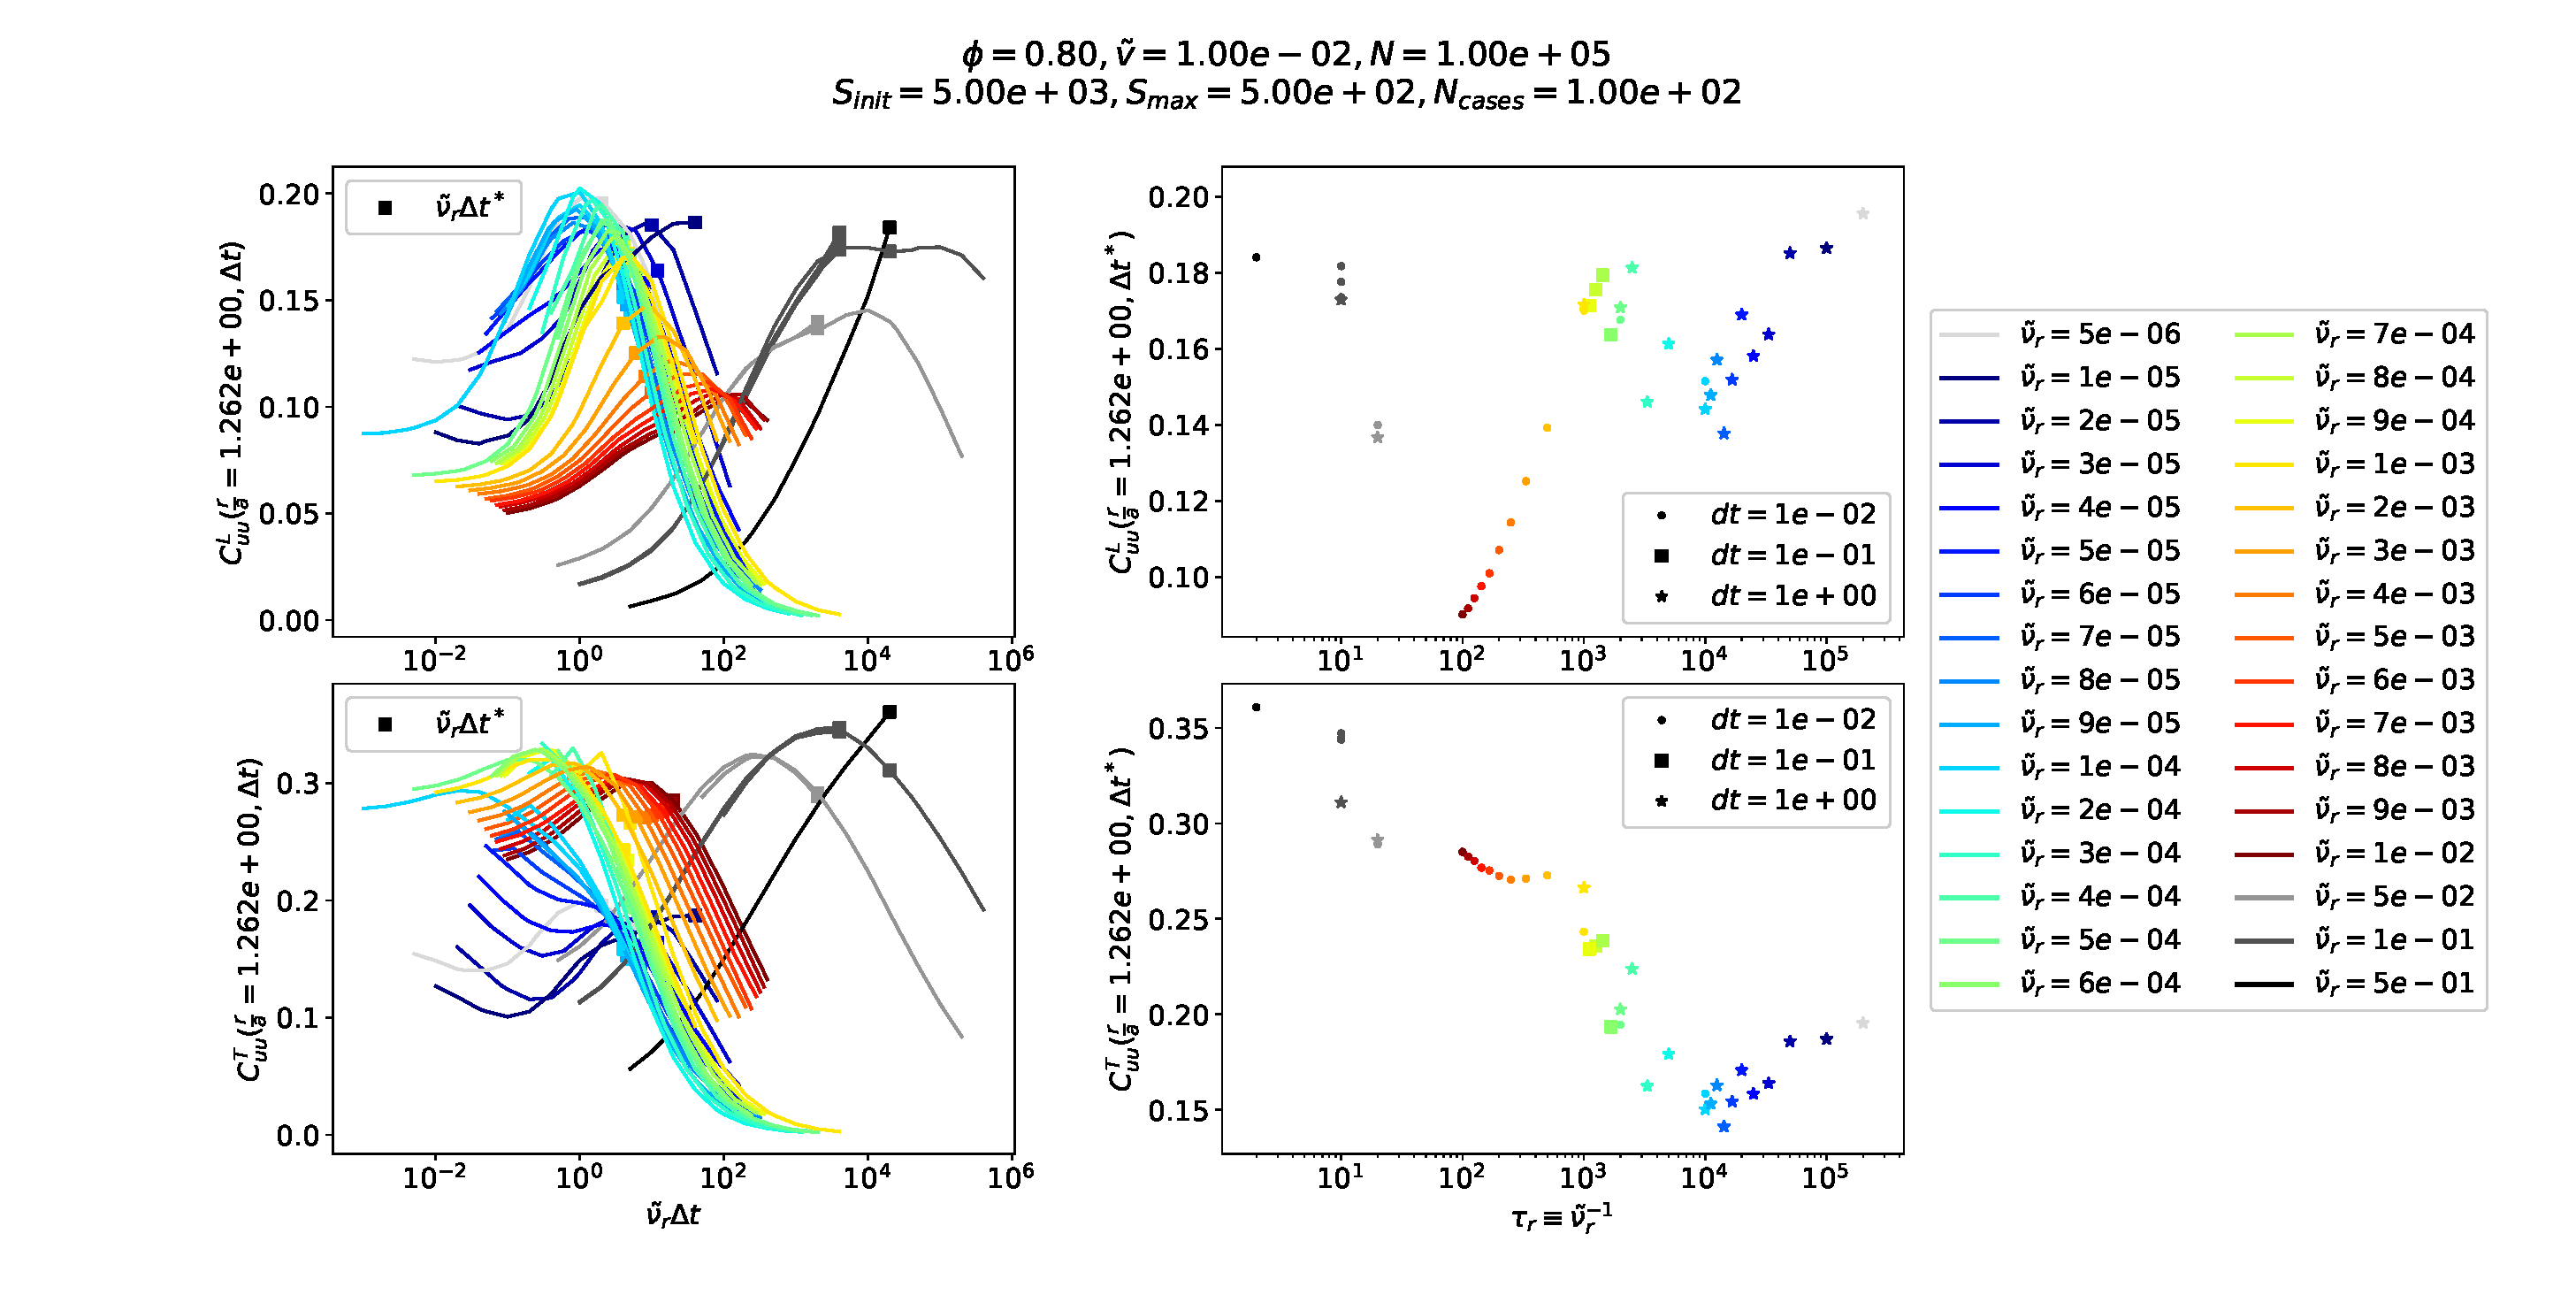
\includegraphics[width=0.8\linewidth]{CuuLCuuT_Dk8000_Vj1000_Nq1000_Io5000_Mn1000_Cn5000_separate.eps}
  \vspace{-0.2cm}
  \caption{Comparison of longitudinal and transversal displacement correlations at grid size distance, $C_{uu}^L(\Delta t)$ and $C_{uu}^T(\Delta t)$, at packing fraction $\phi=0.80$ and self-propulsion velocity $\tilde{v}=1\cdot10^{-2}$.}
\end{figure}

\vspace{-0.3cm}
Hard to interprete these raw data... \only<2>{$\Rightarrow$ look at the ratio!}
}

\only<3>{
\vspace{-0.2cm}
\begin{figure}[h!]
  \centering
  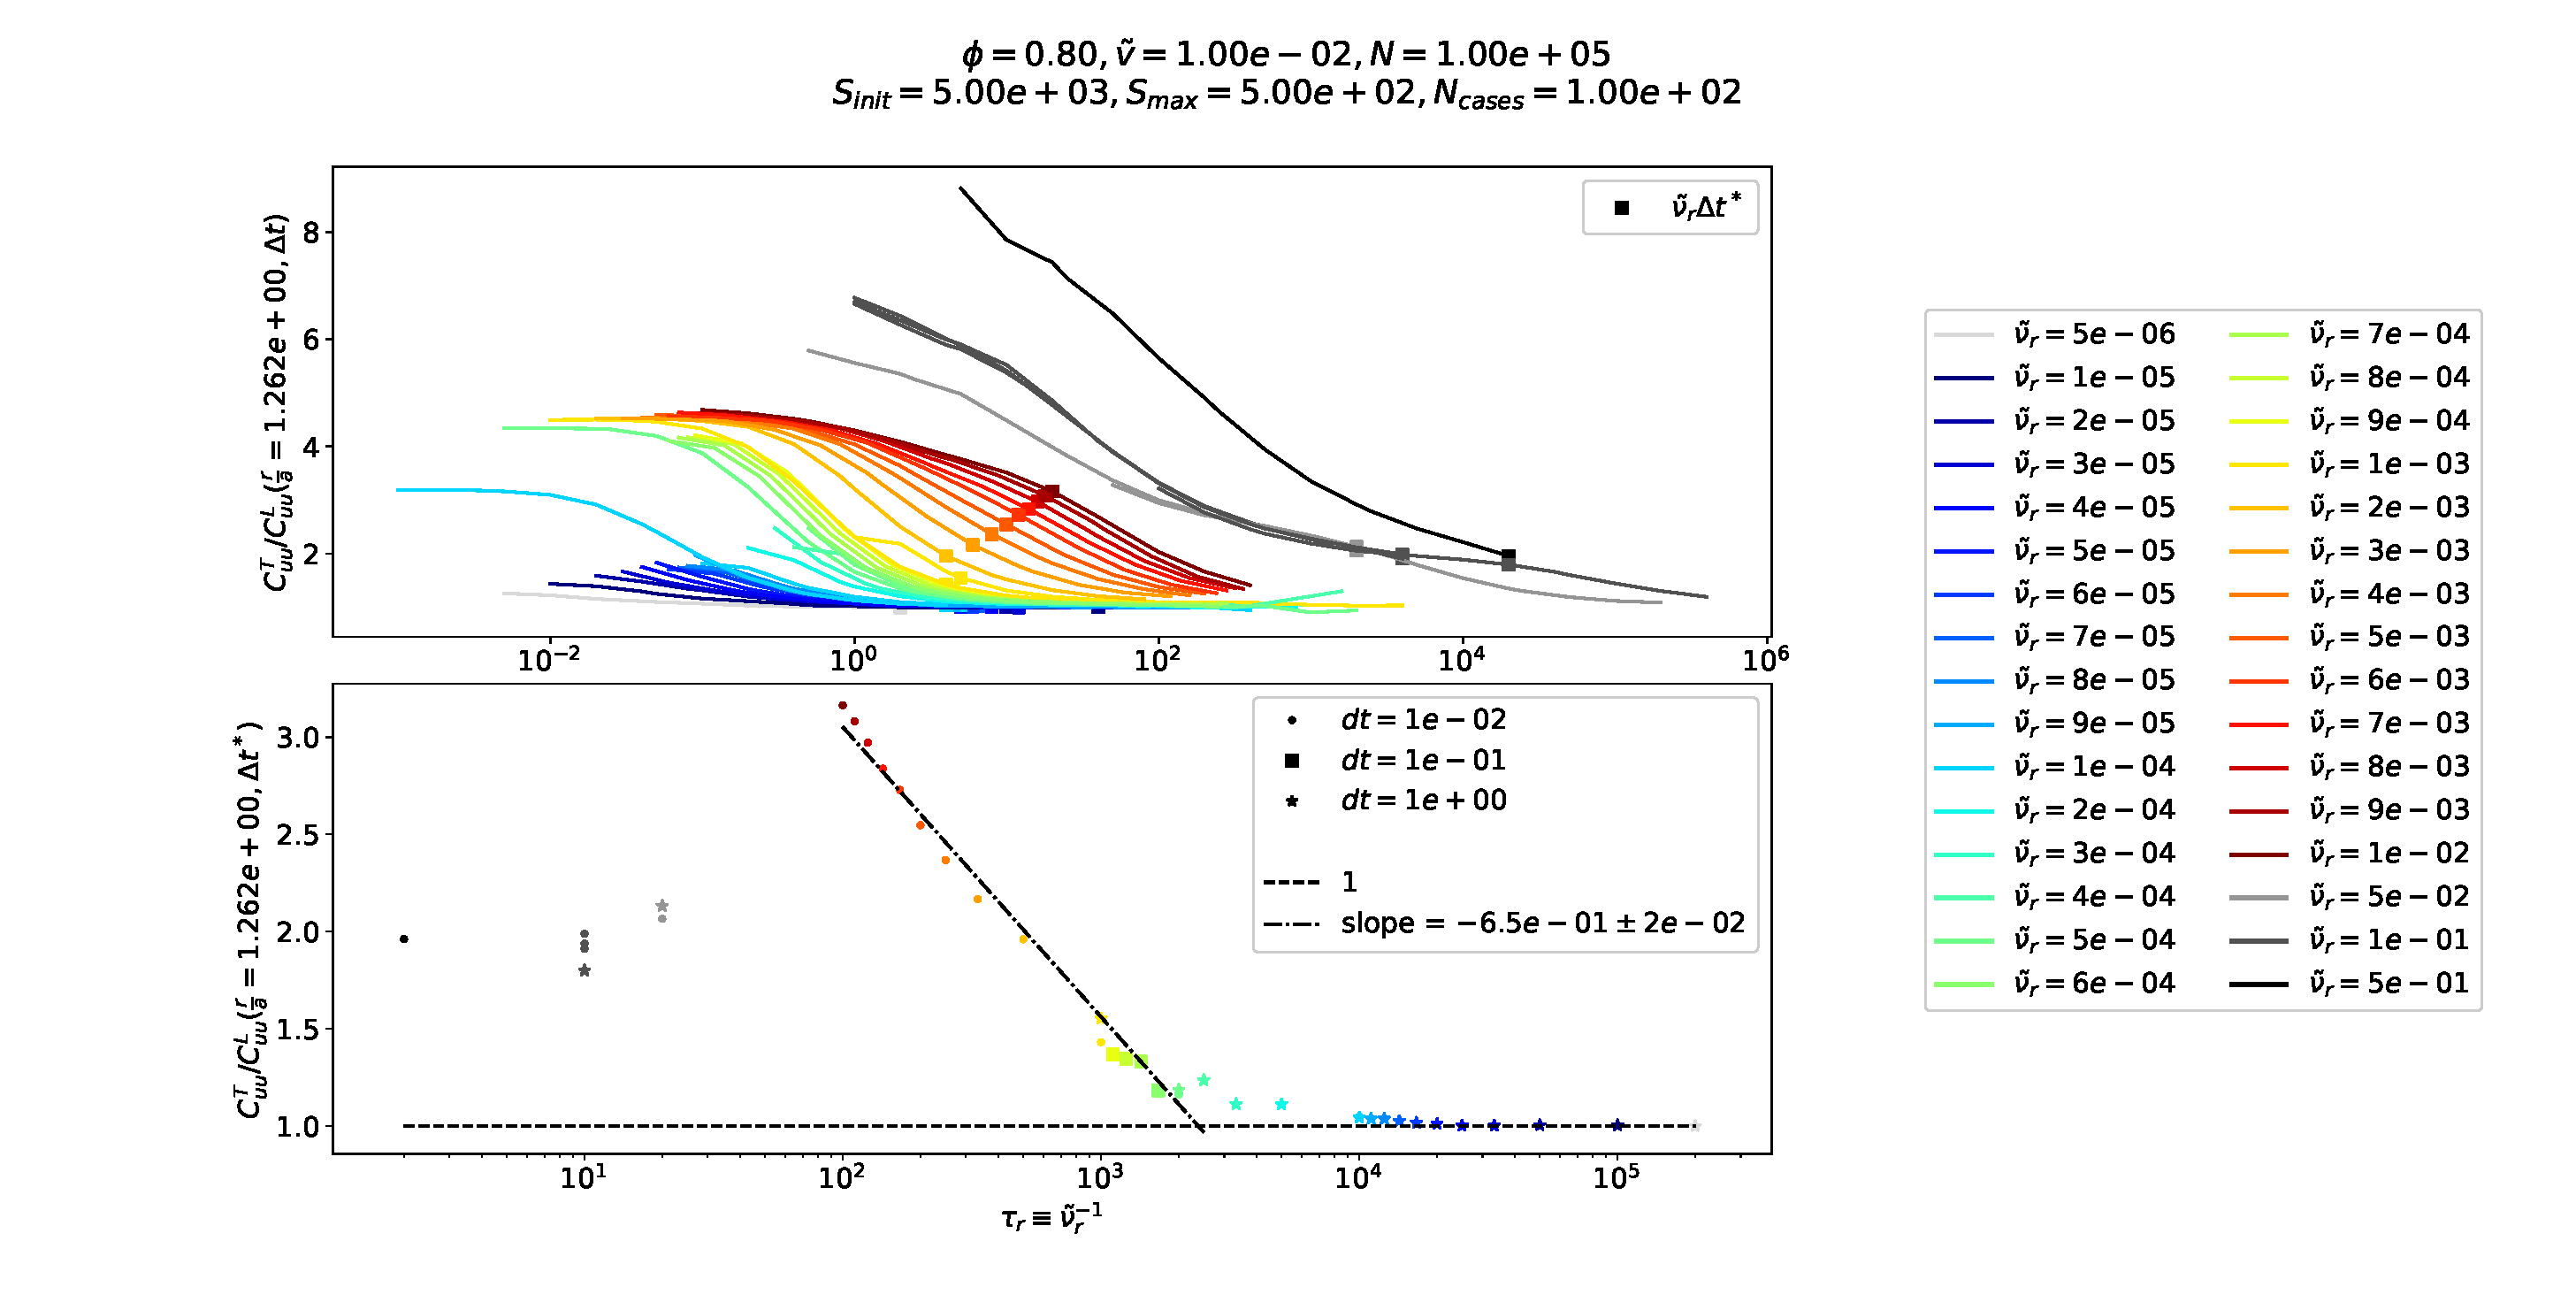
\includegraphics[width=0.8\linewidth]{CuuLCuuT_Dk8000_Vj1000_Nq1000_Io5000_Mn1000_Cn5000.eps}
  \vspace{-0.2cm}
  \caption{Comparison of ratio of transversal and longitudinal displacement correlations at grid size distance, $C_{uu}^T/C_{uu}^L(\Delta t)$, at packing fraction $\phi=0.80$ and self-propulsion velocity $\tilde{v}=1\cdot10^{-2}$.}
\end{figure}

\vspace{-0.3cm}
\begin{itemize}
  \item[$\rightarrow$] Clear change of $C_{uu}^T/C_{uu}^L(\Delta t^*, \text{Pe})$ slope at MIPS.
  \item[$\rightarrow$] $C_{uu}^T/C_{uu}^L(\Delta t^* > 1$ in homogeneous fluid regime and $C_{uu}^T/C_{uu}^L(\Delta t^* = 1$ in phase separated state.
\end{itemize}
}

\end{frame}

\begin{frame}{Directional displacement correlations with varying $\tilde{v}$}

\vspace{-0.2cm}
\begin{figure}[h!]
  \centering
  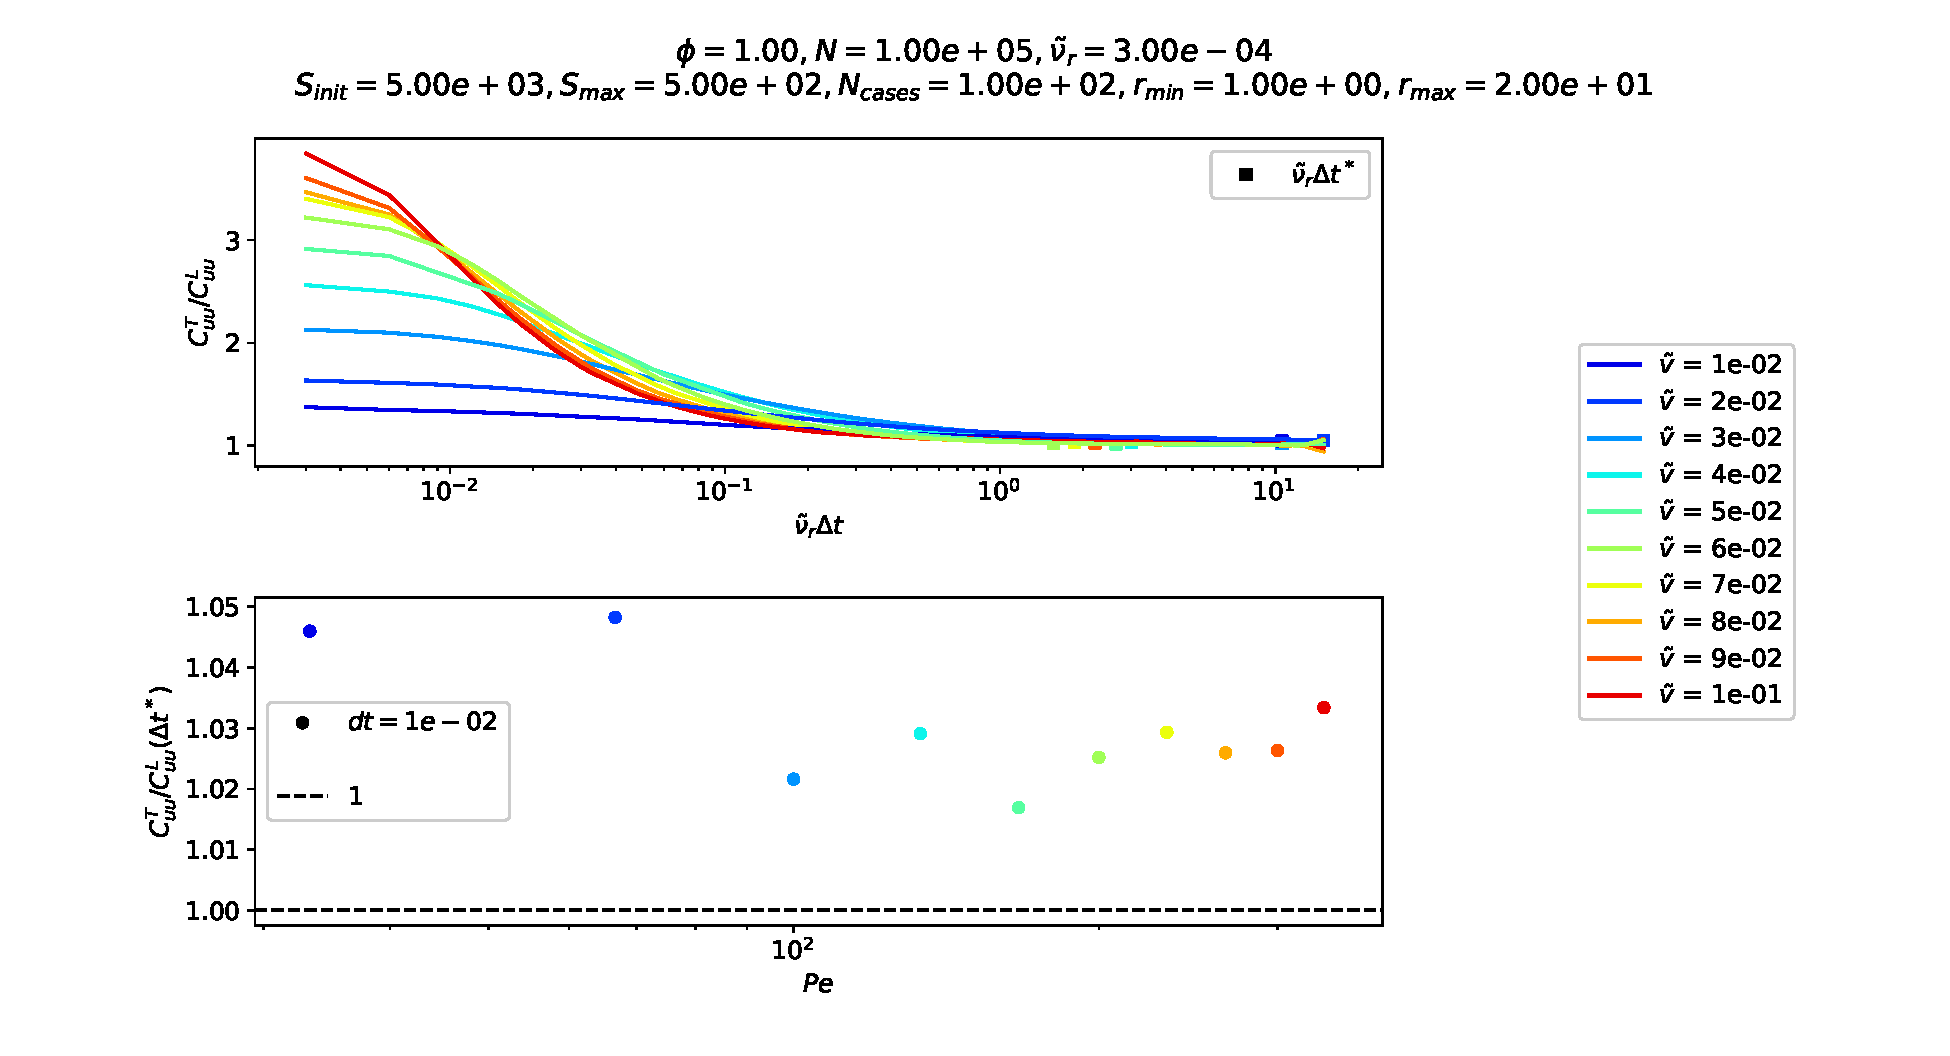
\includegraphics[width=0.8\linewidth]{CuuLCuuT_Dl1000_Rh3000_Nq1000_Io5000_Mn1000_Cn5000.eps}
  \vspace{-0.2cm}
  \caption{Comparison of ratio of transversal and longitudinal displacement correlations at grid size distance, $C_{uu}^T/C_{uu}^L(\Delta t)$, at packing fraction $\phi=1.00$ and rotation diffusion constant $\tilde{\nu}_r=3\cdot10^{-4}$.}
\end{figure}

\vspace{-0.5cm}
\begin{itemize}
  \item[$\rightarrow$] No clear change of $C_{uu}^T/C_{uu}^L(\Delta t^*, \text{Pe})$ slope at MIPS.
  \item[$\rightarrow$] $C_{uu}^T/C_{uu}^L(\Delta t^*) \sim 1$ in both the homogeneous fluid regime and phase separated state.
\end{itemize}

\end{frame}

\begin{frame}{Overview (varying $\tilde{\nu}_r$)}

\vspace{-0.2cm}

\begin{figure}[h!]
  \centering
  \only<1>{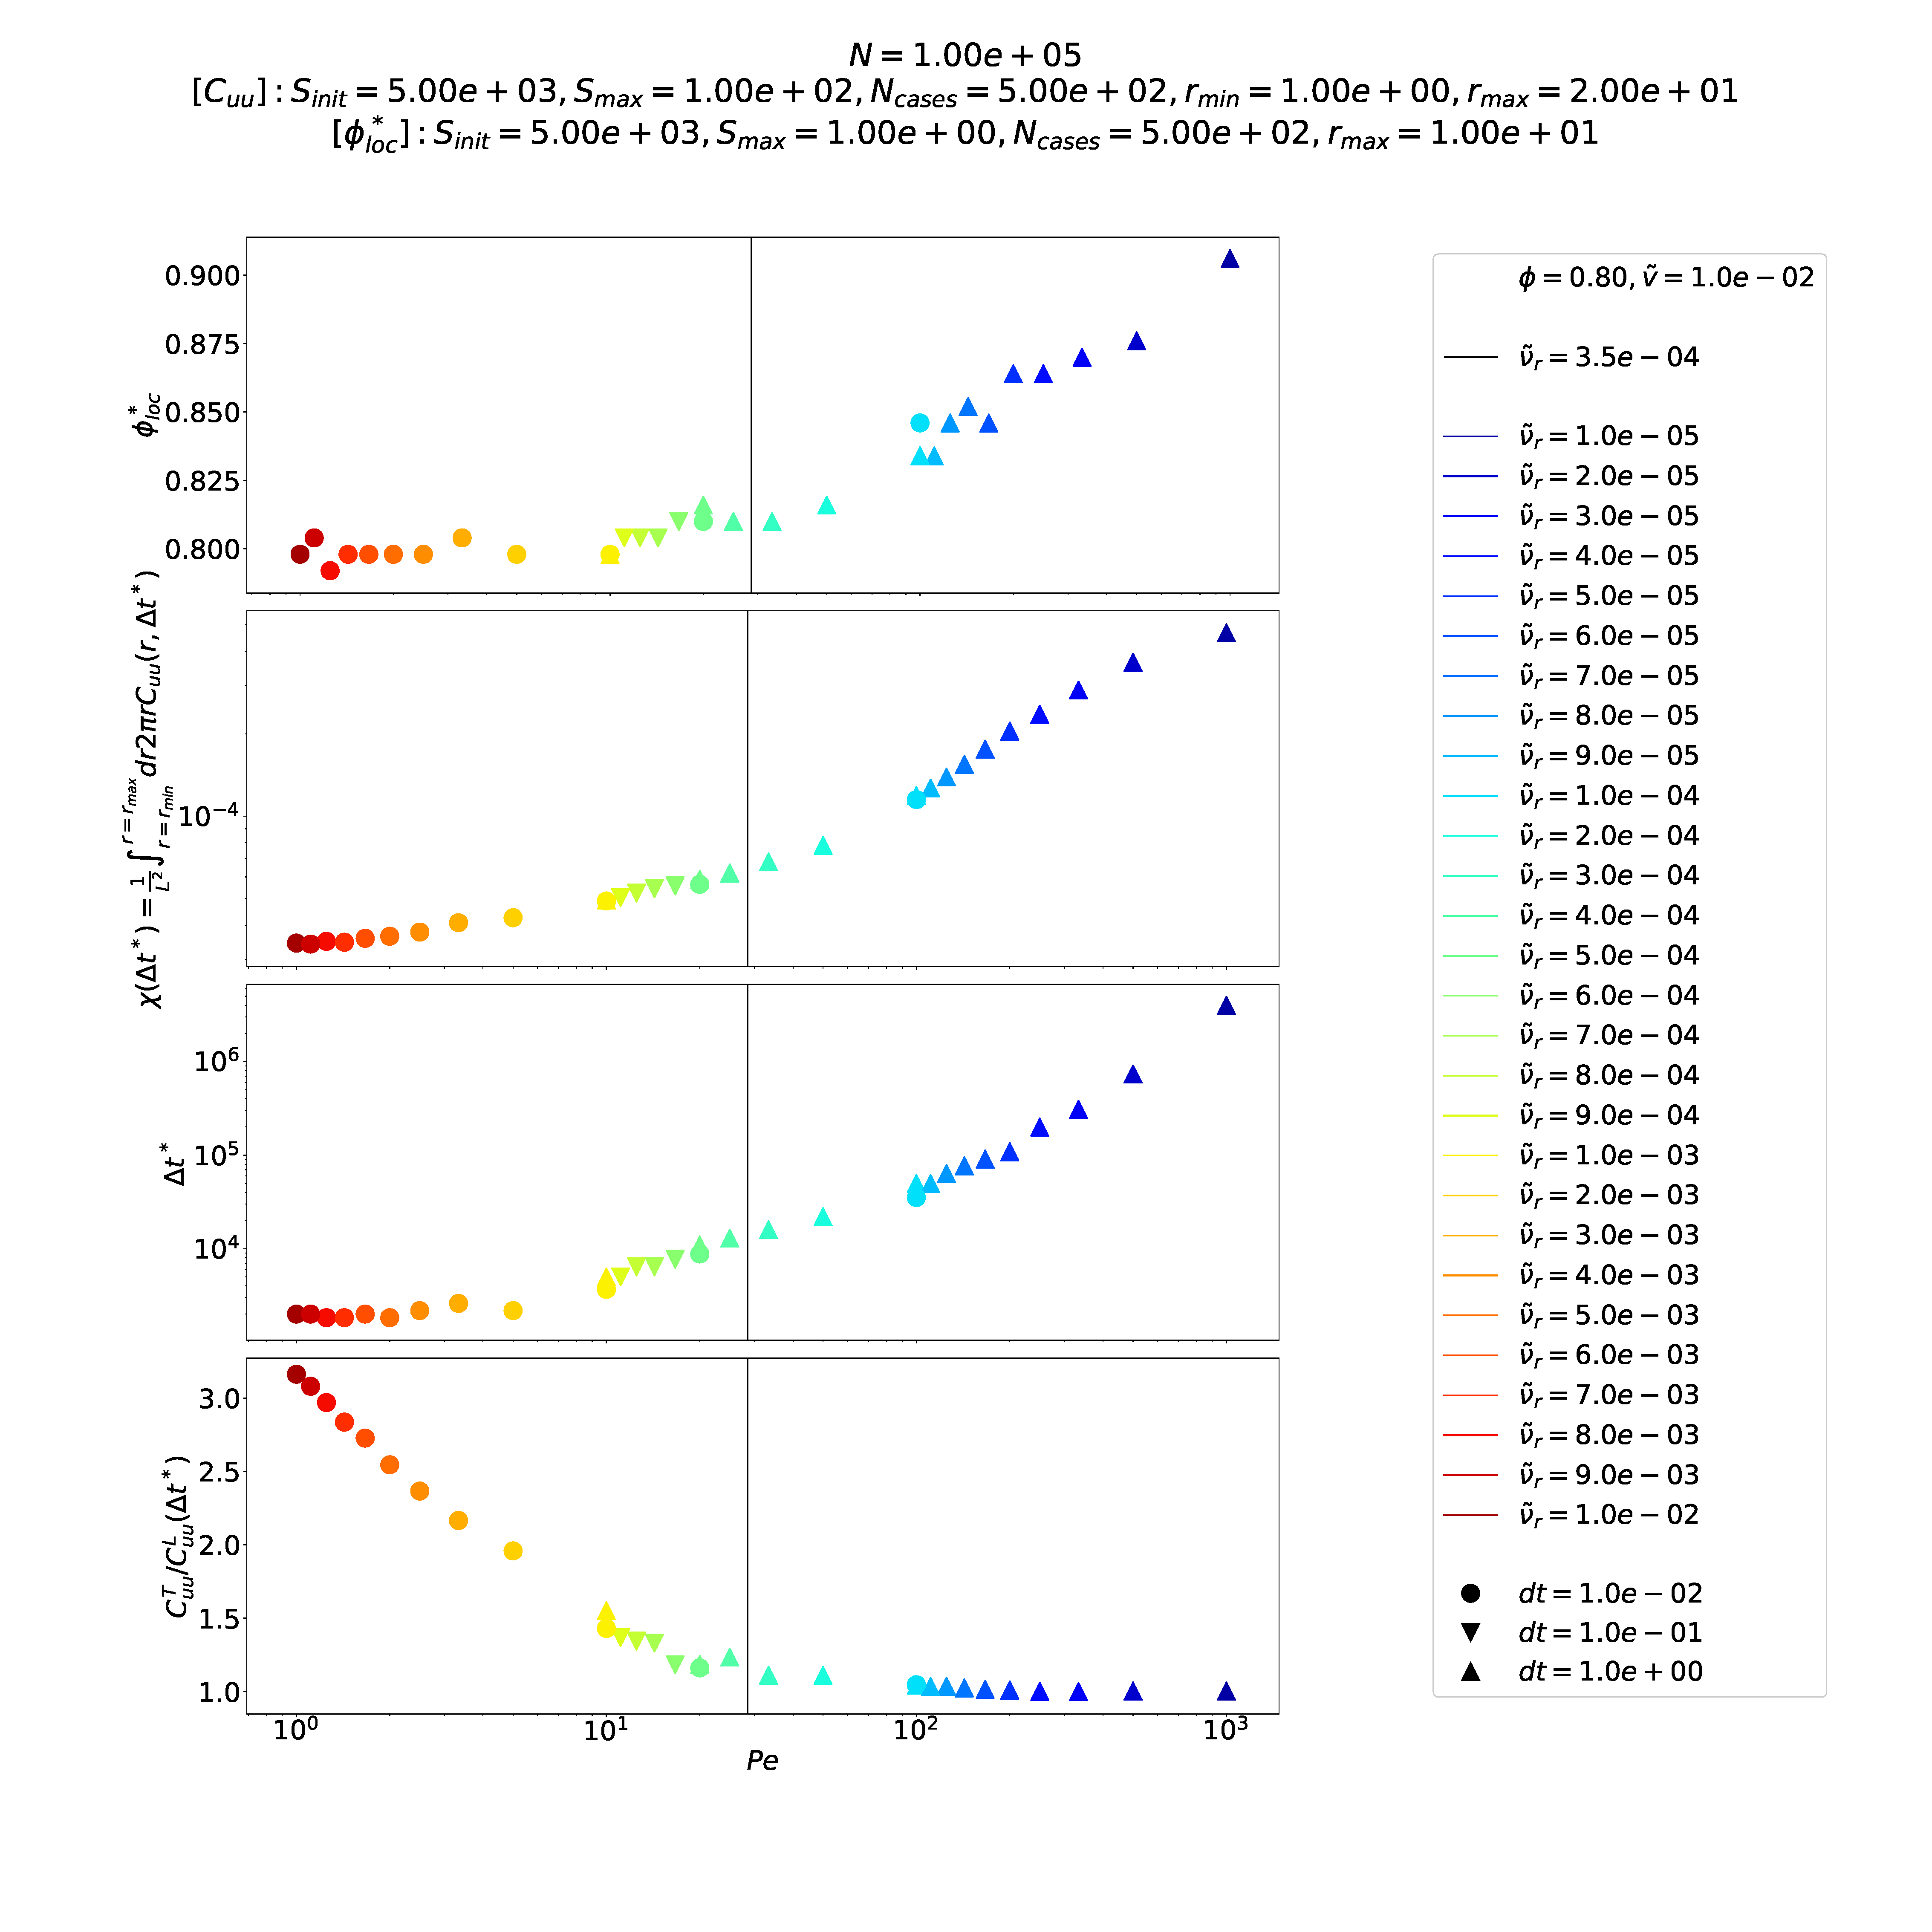
\includegraphics[width=0.55\linewidth]{comparison_Dk8000_Vj1000_dt.eps}}
  \only<2>{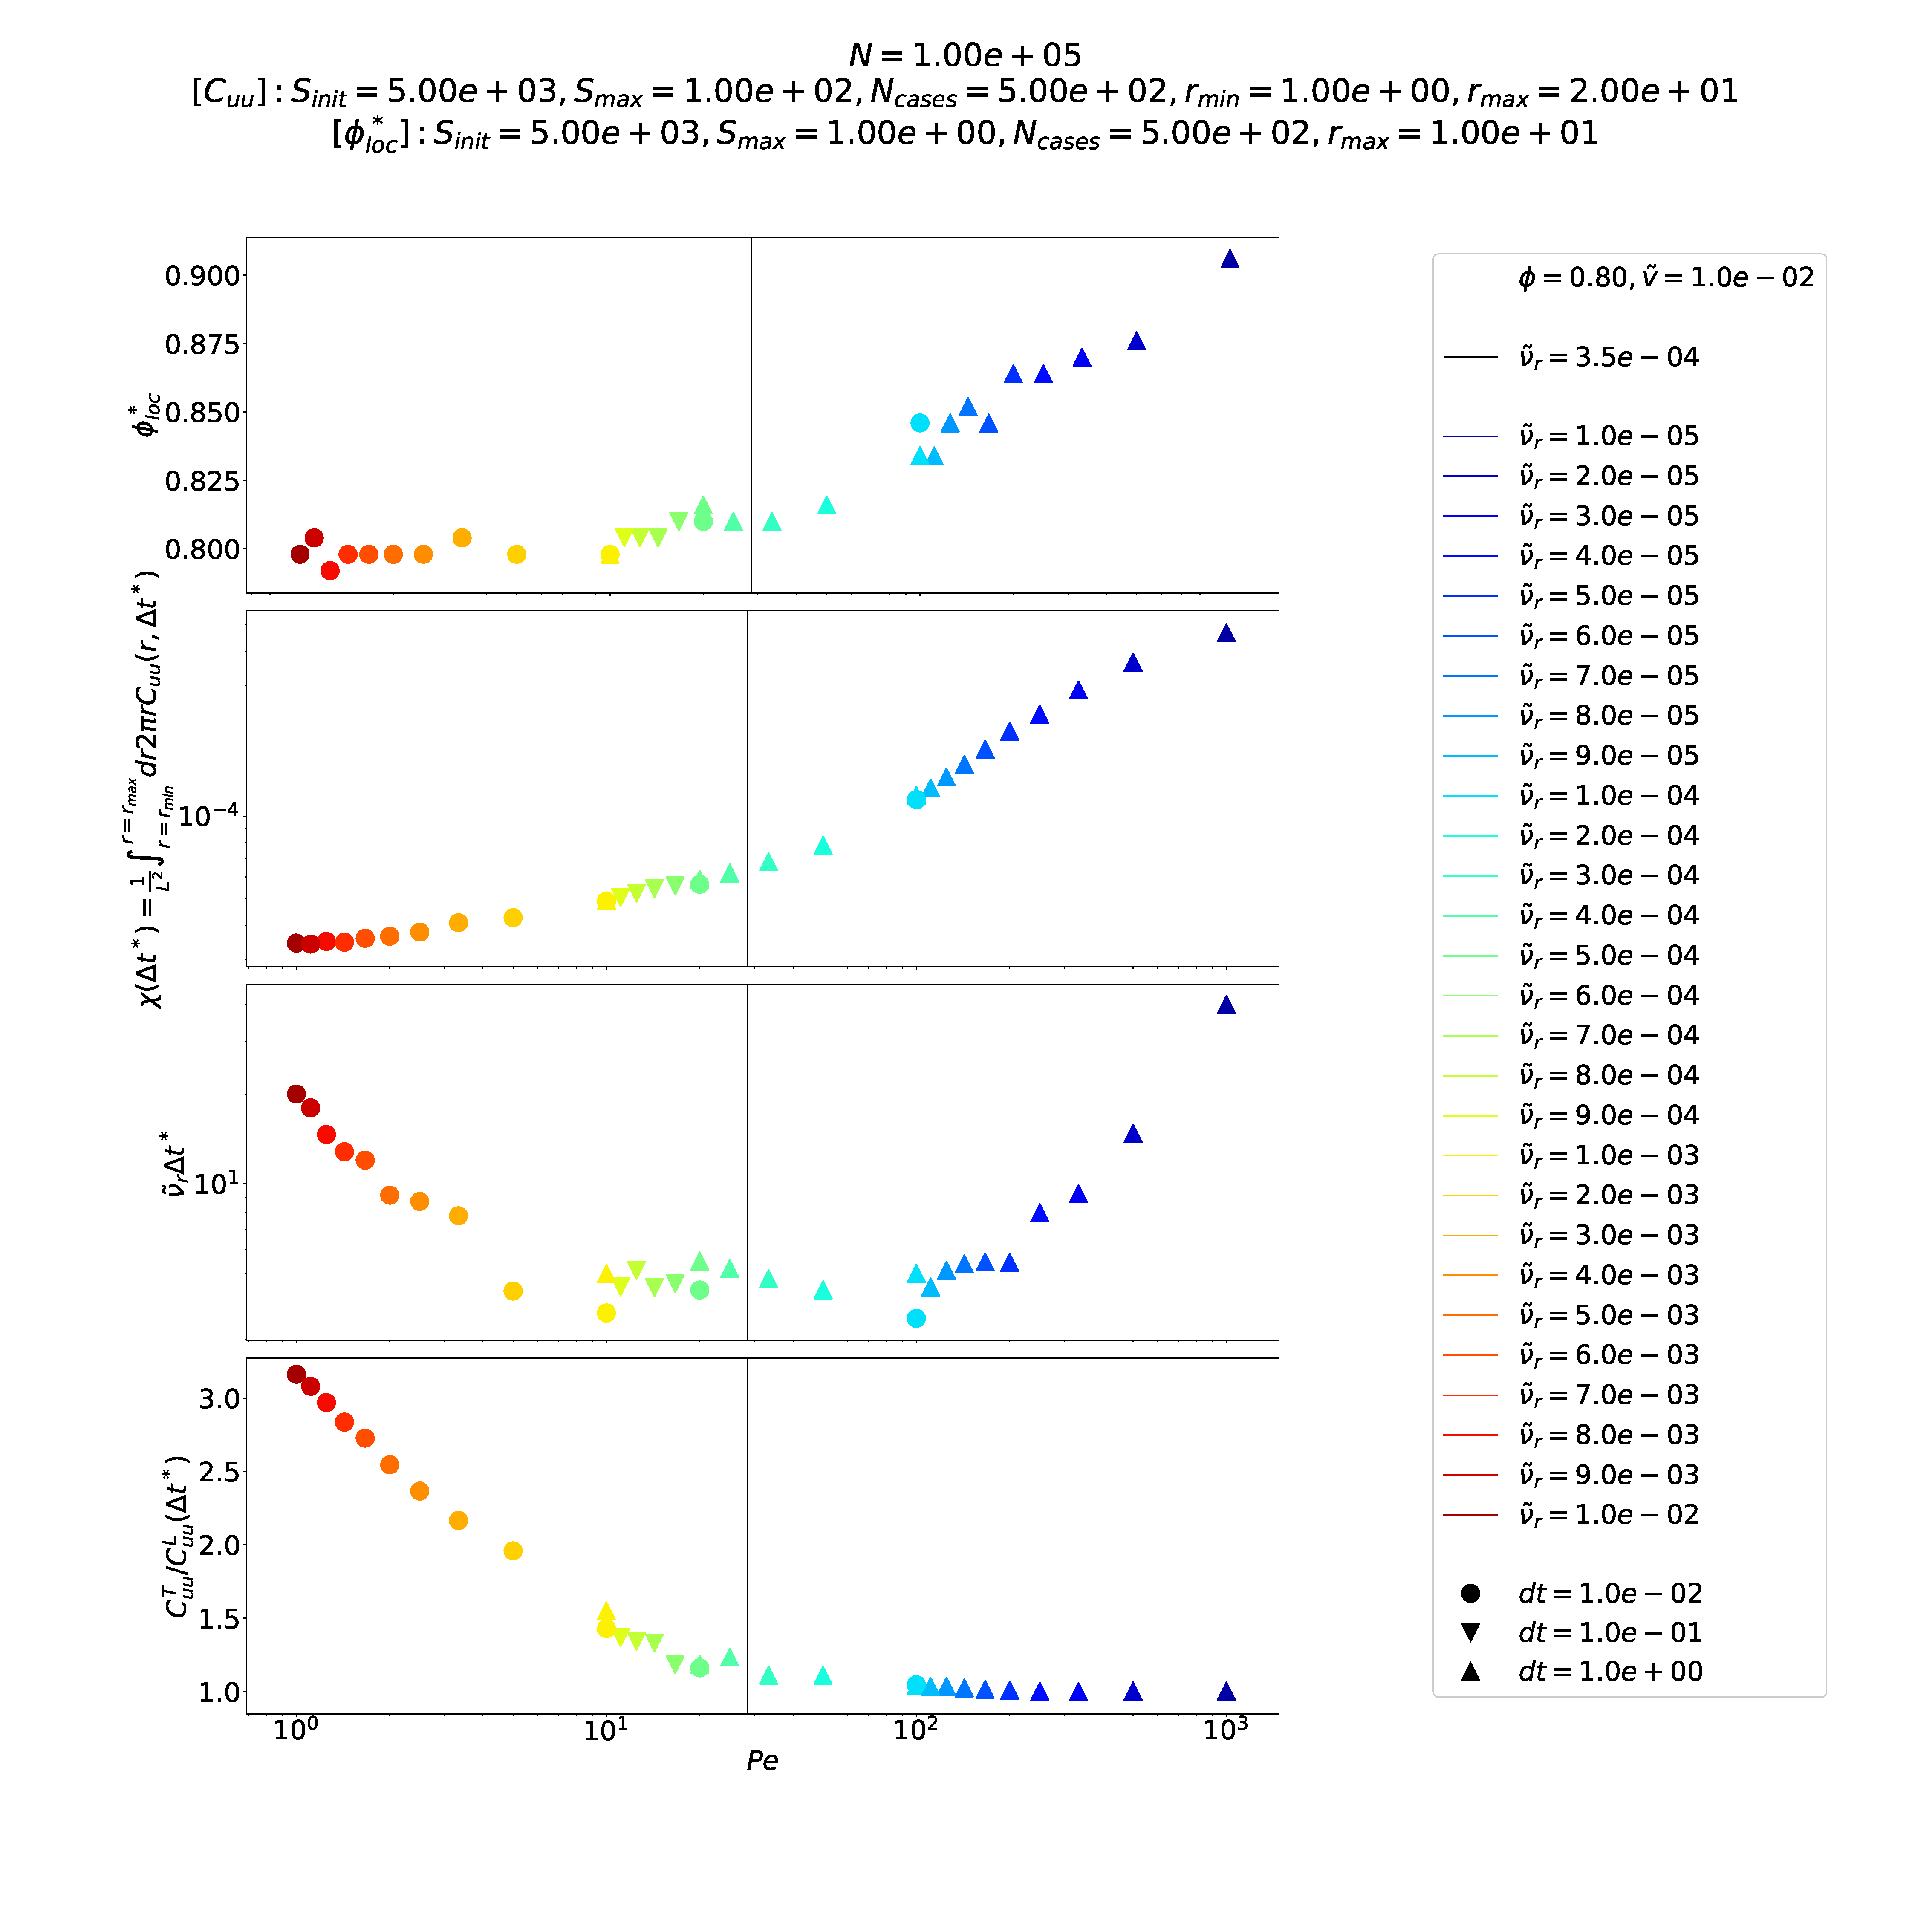
\includegraphics[width=0.55\linewidth]{comparison_Dk8000_Vj1000_drdt.eps}}
  \vspace{-0.6cm}
  \only<1>{\caption{Overview plot of most probable local density $\phi_{loc}^*$, maximum cooperativity $\chi(\Delta t^*)$, time of maximum cooperativity $\Delta t^*$ and ratio of transversal and longitudinal displacement correlations at time of maximum cooperativity and grid size distance $C_{uu}^T/C_{uu}^L(\Delta t^*)$, at packing fraction $\phi=0.80$ and self-propelling velocity $\tilde{v}=1\cdot10^{-2}$.}}
  \only<2>{\caption{Overview plot of most probable local density $\phi_{loc}^*$, maximum cooperativity $\chi(\Delta t^*)$, number of rotations of maximum cooperativity $\tilde{\nu}_r\Delta t^*$ and ratio of transversal and longitudinal displacement correlations at time of maximum cooperativity and grid size distance $C_{uu}^T/C_{uu}^L(\Delta t^*)$, at packing fraction $\phi=0.80$ and self-propelling velocity $\tilde{v}=1\cdot10^{-2}$.}}
\end{figure}

\end{frame}

\begin{frame}{Overview (varying $\tilde{v}$)}

\vspace{-0.2cm}

\begin{figure}[h!]
  \centering
  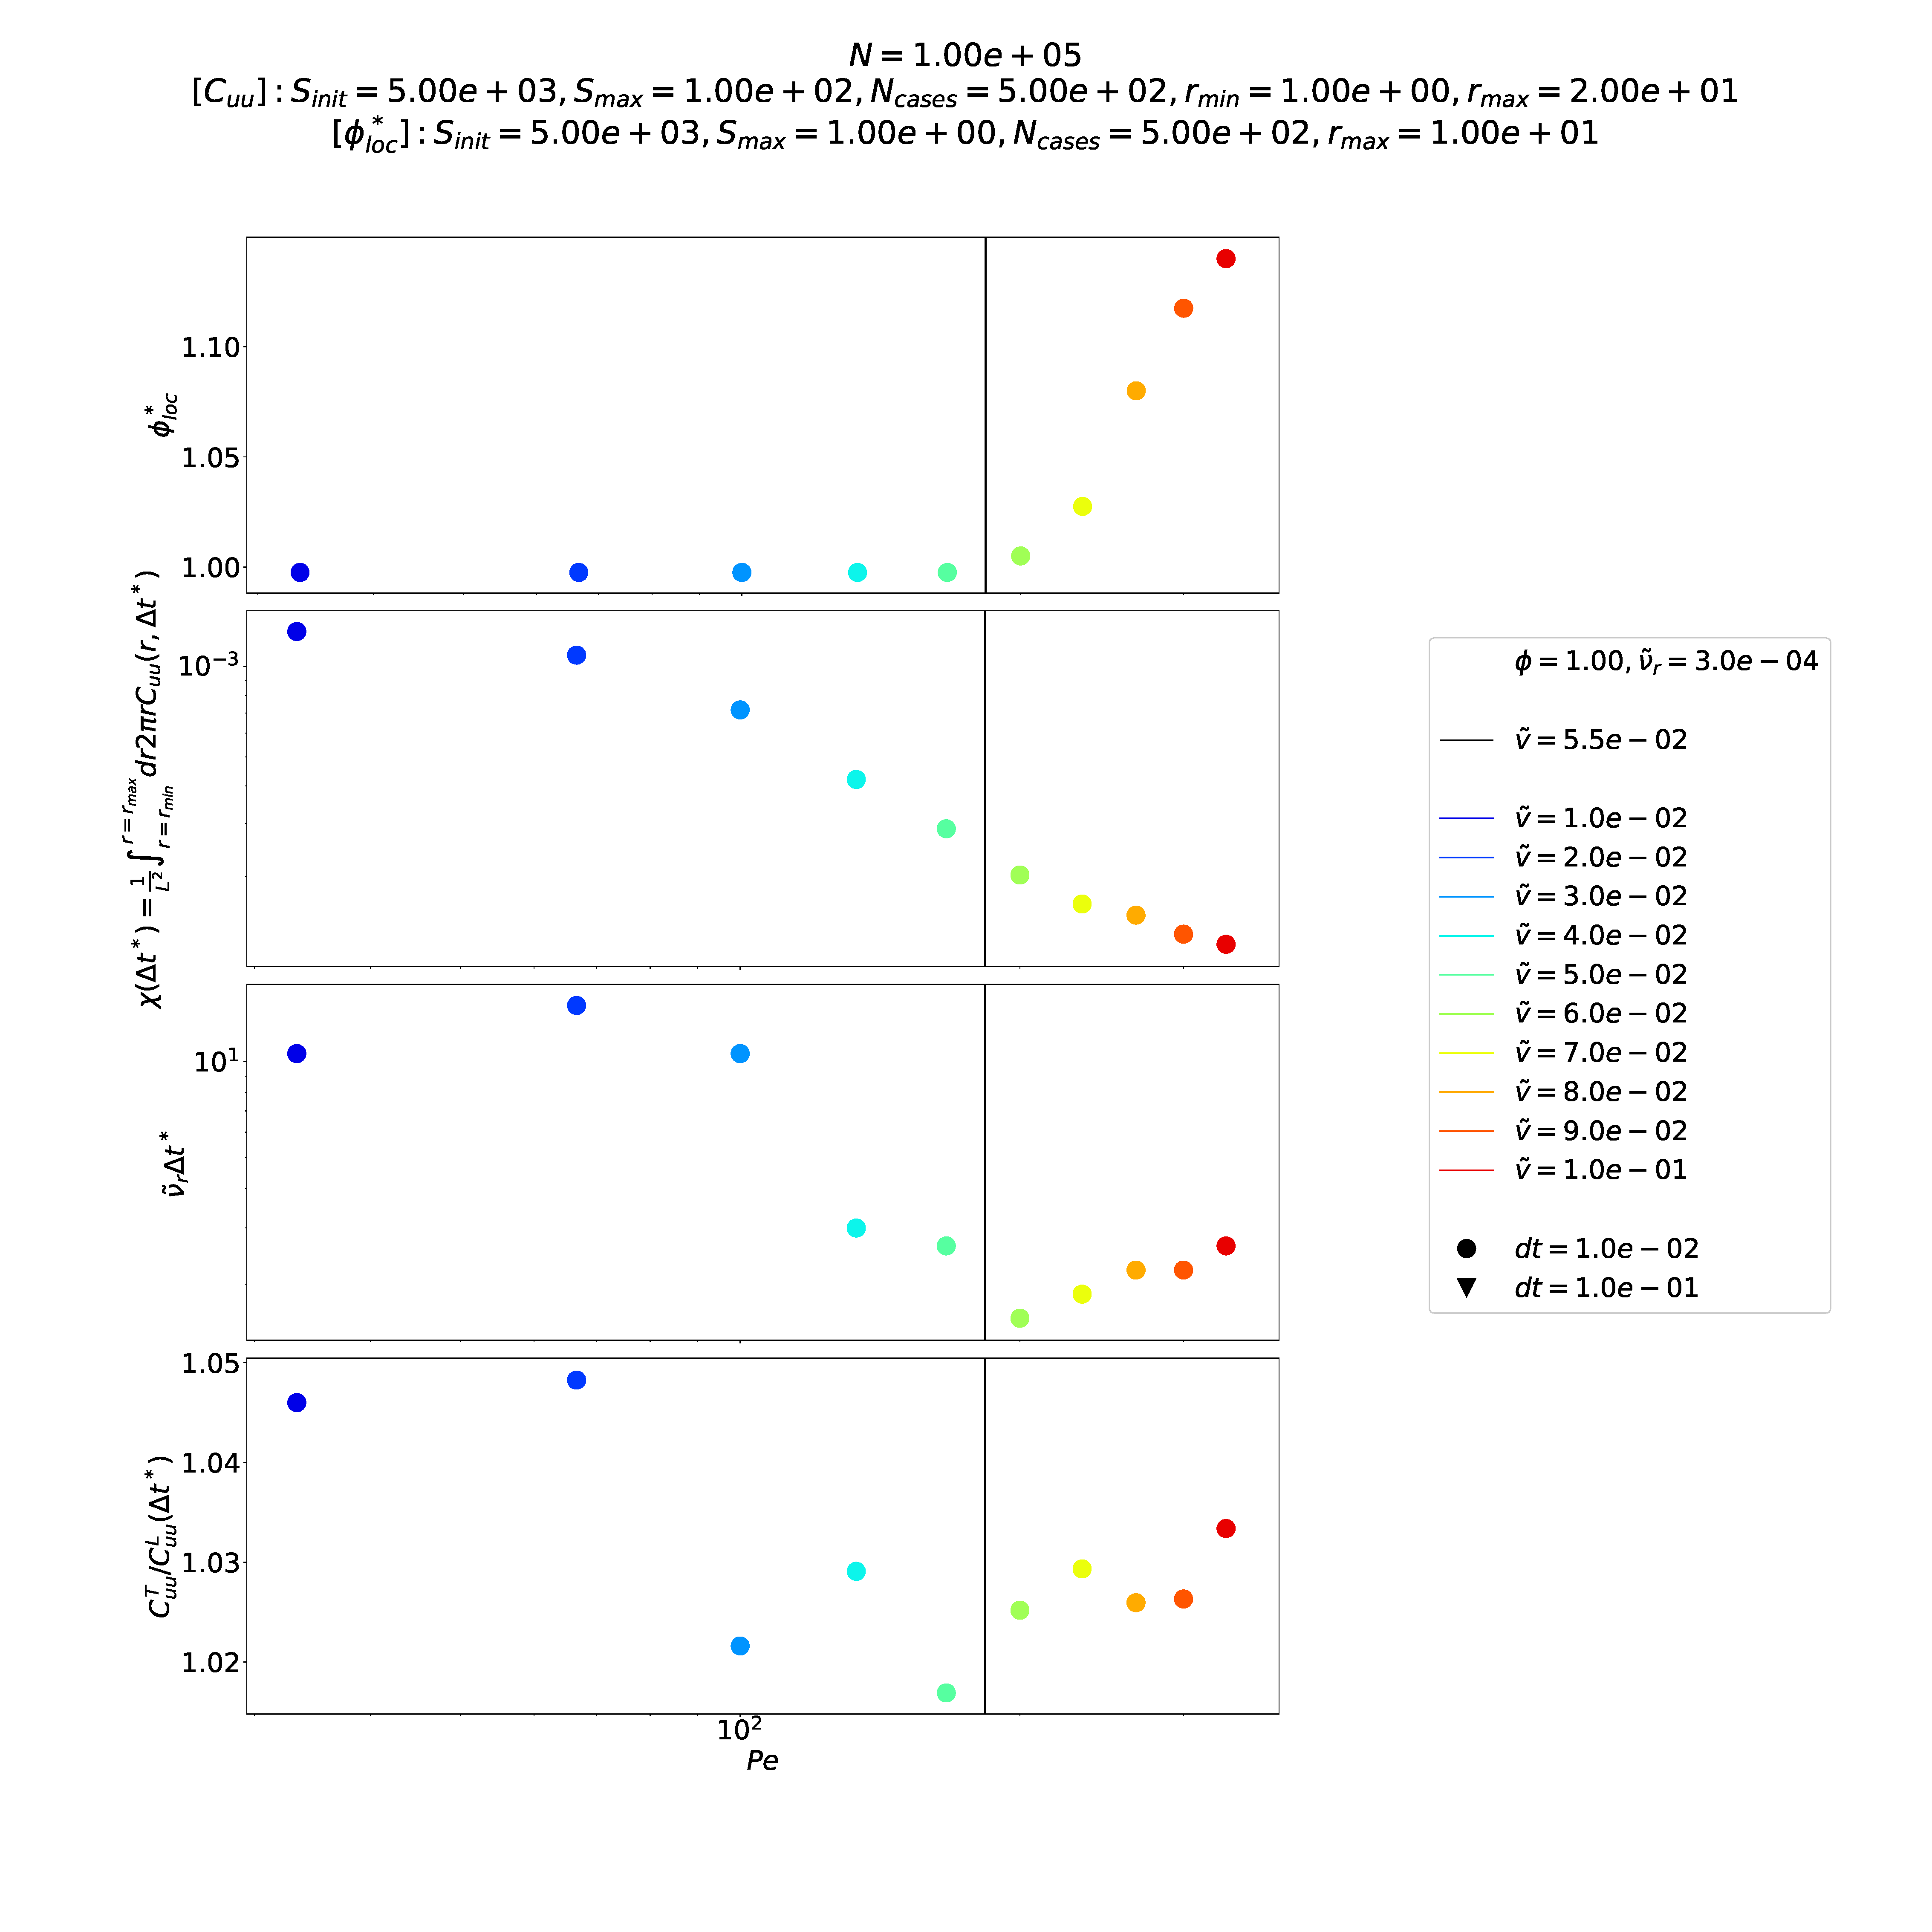
\includegraphics[width=0.55\linewidth]{comparison_Dl1000_Rh3000_drdt.eps}
  \vspace{-0.6cm}
  \caption{Overview plot of most probable local density $\phi_{loc}^*$, maximum cooperativity $\chi(\Delta t^*)$, number of rotations of maximum cooperativity $\tilde{\nu}_r\Delta t^*$ and ratio of transversal and longitudinal displacement correlations at time of maximum cooperativity and grid size distance $C_{uu}^T/C_{uu}^L(\Delta t^*)$, at packing fraction $\phi=1.00$ and rotation diffusion constant $\tilde{\nu}_r=3\cdot10^{-4}$.}
\end{figure}

\end{frame}

\subsection{Shear strain correlations}

\begin{frame}{Trajectories at low activity}

\vspace{-0.25cm}
\insertmovie{0.6}{t_Dk8000_Vj1000_Ri7000_Nq1000_Ll0000_Io5000_Mo1000_Pn1000}{Trajectories at low activity ($\tilde{\nu}_r = 7\cdot10^{-3}$) with $\Delta t = 1\cdot10^3$.}

\end{frame}

\begin{frame}{Trajectories at high activity}

\vspace{-0.25cm}
\insertmovie{0.6}{t_Dk8000_Vj1000_Rg2000_Nq1000_Ll0000_Io5000_Mo1000_Pl1000}{Trajectories at high activity ($\tilde{\nu}_r = 2\cdot10^{-5}$) with $\Delta t = 1\cdot10^3$.}

\end{frame}

\begin{frame}{Linearised shear strain}

$\vec{u}(\vec{r}, t, t + \Delta t) = \begin{pmatrix} u_x(\vec{r}, t, t + \Delta t) \\ u_y(\vec{r}, t, t + \Delta t) \end{pmatrix} \equiv$ displacement of particle at position $\vec{r}$ between times $t$ and $t + \Delta t$\\

Accumulated shear strain at position $\vec{r}$ between times $t$ and $t  + \Delta t$
\begin{align*}
&\varepsilon_{xy}(\vec{r}, t, t + \Delta t)\\
\underset{\frac{||\vec{u}||}{L} \ll 1}{=} &\frac{1}{2}\left(\frac{\partial}{\partial x}u_y(\vec{r}, t, t + \Delta t) + \frac{\partial}{\partial y}u_x(\vec{r}, t, t + \Delta t)\right)
\end{align*}
with $L$ characteristic length of system.

\end{frame}

\begin{frame}{Shear strain correlation}

\begin{align*}
C_{\varepsilon_{xy}\varepsilon_{xy}}(\Delta \vec{r}, \Delta t) &= \left<\varepsilon_{xy}(\vec{r}+\Delta\vec{r}, t, t + \Delta t)\varepsilon_{xy}(\vec{r}, t, t + \Delta t)\right>
\only<2->{
\\
&= \frac{\int dt \int d^2\vec{r}~ \varepsilon_{xy}(\vec{r}, t, t+\Delta t)\varepsilon_{xy}(\vec{r} + \Delta \vec{r}, t, t+\Delta t)}{\int dt \int d^2\vec{r}~ |\varepsilon_{xy}(\vec{r}, t, t+\Delta t)|^2}
}
\only<3->{
\\
&= \frac{\mathcal{F}^{-1}\{\int dt~ |\mathcal{F}\{\varepsilon_{xy}\}(\vec{k}, t, t + \Delta t)|^2\}(\Delta \vec{r}, \Delta t)}{\int dt \int d^2\vec{r}~ ||\varepsilon_{xy}(\vec{r}, t, t+\Delta t)||^2}
}
\end{align*}

\end{frame}

\begin{frame}{Projection of shear strain correlation}

\blfootnote{\fullcite{illing2016strain}}

Symmetrised gradient $\Rightarrow$ four-fold symmetry of $C_{\varepsilon_{xy}\varepsilon_{xy}}(\Delta \vec{r}, \Delta t)$.

\only<2->{
\begin{align*}
C_4^4(\Delta r, \Delta t) = \frac{1}{\pi} &\int_0^{2\pi} d\theta~ \cos(4\theta)~ C_{\varepsilon_{xy}\varepsilon_{xy}}(\Delta\vec{r}\equiv(\Delta r, \theta), \Delta t)
\only<3>{
\\
\underset{\frac{\Delta r}{a} \gg 1}{\propto} &\frac{1}{\Delta r^2}\qquad\text{(elastic medium)}
}
\end{align*}
}
\only<3>{
with $a \equiv$ average interparticle distance.
}

\end{frame}

\begin{frame}{Real space method}

Shear strains are evaluated on a grid to calculate their correlations.
\begin{align*}
\vec{u}(\vec{r}_i, t, t + \Delta t) \xrightarrow[\substack{\text{coarse-graining}\\\text{(Gaussian)}}]{} \varepsilon_{xy,ij}(t, t + \Delta t) \only<2>{\xrightarrow[\text{FFT}]{} C_{\varepsilon_{xy}\varepsilon_{xy}, ij}}
\end{align*}

\end{frame}

\begin{frame}{Shear strain map at high activity (real space method)}

\vspace{-0.2cm}
\begin{figure}[h!]
  \centering
  \includegraphics[width=0.85\linewidth]{Cssb_Dk8000_Vj1000_Rg2000_Nq1000_Io5000_Tl1000_Ml1000_Cn5000_RCUTl2000_SIGMl2000.eps}
  \vspace{-0.6cm}
  \caption{Shear strain map $\varepsilon_{xy}(\vec{r}, t, t + \Delta t)$ and corresponding shear strain correlations $C_{\varepsilon_{xy}\varepsilon_{xy}}(\Delta\vec{r}, \Delta t)$, at packing fraction $\phi=0.80$, self-propulsion velocity $\tilde{v}=1\cdot10^{-2}$ and rotation diffusion constant $\tilde{\nu}_r=2\cdot10^{-5}$.}
\end{figure}

\vspace{-0.5cm}
\begin{itemize}
  \item[$\rightarrow$] Highest strain values at phase interface.
  \item[$\rightarrow$] Quadropular symmetry of shear strain correlations.
  \item[$\rightarrow$] Shear strain correlations blured because of gas phase.
\end{itemize}

\end{frame}

\begin{frame}{Real space method}

Shear strains are evaluated on a grid to calculate their correlations.
\begin{align*}
\vec{u}(\vec{r}_i, t, t + \Delta t) \xrightarrow[\substack{\text{coarse-graining}\\\text{(Gaussian)}}]{} \varepsilon_{xy,ij}(t, t + \Delta t) \xrightarrow[\text{FFT}]{} C_{\varepsilon_{xy}\varepsilon_{xy}, ij}
\end{align*}

Significant downside: coarse-graining step is particularly long, execution time = days to get good statistics.\\

\only<2>{$\Rightarrow$ turn to a Fourier space based method to speed up this part.}

\end{frame}

\begin{frame}{Collective mean square displacements}

\blfootnote{\fullcite{illing2016strain}}
\blfootnote{\fullcite{leonforte2005continuum}}

\vspace{-1cm}

\begin{align*}
\vec{u}(\vec{r}, t, t + \Delta t) \xrightarrow[\text{Fourier transform}]{} \tilde{\vec{u}}(\vec{k}, t, t + \Delta t)
\end{align*}

\only<2->{
\begin{align*}
C^{\perp}(\vec{k}, \Delta t) &= ||\vec{k}||^{-2}\left<||\vec{k}\wedge\tilde{\vec{u}}(\vec{k}, t, t  +\Delta t) ||^2\right> \only<3>{\xrightarrow[\text{isotropy}]{}C^{\perp}(k, \Delta t)}\\
C^{||}(\vec{k}, \Delta t) &=   ||\vec{k}||^{-2}\left<||\vec{k}\cdot\tilde{\vec{u}}(\vec{k}, t, t  +\Delta t) ||^2\right> \only<3>{\xrightarrow[\text{isotropy}]{}C^{||}(k, \Delta t)}
\end{align*}
respectivement the transversal and longitudinal collective mean square displacements (CMSD).
}

\end{frame}

\begin{frame}{CMSD and shear strain correlations}

\blfootnote{\fullcite{illing2016strain}}
\blfootnote{\fullcite{leonforte2005continuum}}

\vspace{-1cm}

\begin{align*}
C_{\varepsilon_{xy}\varepsilon_{xy}}(\Delta \vec{r}, \Delta t) = \mathcal{F}^{-1}\Big\{&-\frac{k_x^2k_y^2}{k^2}\left(C^{\perp}(k, \Delta t) - C^{||}(k, \Delta t)\right)\\
&+ \frac{k^2}{4}C^{\perp}(k, \Delta t)\Big\}(\Delta \vec{r}, \Delta t)
\end{align*}

\only<2->{
\begin{align*}
&\subalign{&C^{||}(k, \Delta t) = 0 \\ &C^{\perp}(k, \Delta t) \propto k^{-2}} \qquad \text{(incompressible glass)}\\
\only<3>{&\Rightarrow C_{\varepsilon_{xy}\varepsilon_{xy}}(\Delta \vec{r}, \Delta t) \propto \cos(4\theta) \Delta r^{-2}}
\end{align*}
}

\end{frame}

\begin{frame}{CMSD method}

Displacements are put on a grid to calculate shear strain correlations from CMSD.
\begin{align*}
\vec{u}(\vec{r}_i, t, t + \Delta t) \only<1-2>{\xrightarrow[\substack{\text{coarse-graining}\\\text{(average in grid box)}}]{}}\only<3->{\rightarrow} \vec{u}_{ij}(t, t + \Delta t) \only<2->{\xrightarrow[\text{FFT}]{} \tilde{\vec{u}}_{ij}(t, t + \Delta t)}
\only<3->{\rightarrow \text{CMSD}}
\end{align*}

\end{frame}

\begin{frame}{CMSD at high activity}

\vspace{-0.2cm}
\begin{figure}[h!]
  \centering
  \includegraphics[width=0.8\linewidth]{Cttb_Dk8000_Vj1000_Rg2000_Nq1000_Io5000_Tl1000_Mn1000_Cn5000_Bn3000_XN1500_Yn1500.eps}
  \vspace{-0.8cm}
  \caption{Transversal and longitudinal CMSD, $C^{\perp}(k, \Delta t) \equiv \left<||\vec{k}\wedge\tilde{\vec{u}}(\vec{k})||^2\right>/k^2$ and $C^{||}(k, \Delta t) \equiv \left<||\vec{k}\cdot\tilde{\vec{u}}(\vec{k})||^2\right>/k^2$, at packing fraction $\phi=0.80$, self-propulsion velocity $\tilde{v}=1\cdot10^{-2}$ and rotation diffusion constant $\tilde{\nu}_r=2\cdot10^{-5}$.}
\end{figure}

\vspace{-0.5cm}
\begin{itemize}
  \item[$\rightarrow$] $C^{||}(k, \Delta t) \neq 0$.
  \item[$\rightarrow$] $C^{\perp}(k, \Delta t), C^{||}(k, \Delta t) \propto k^{-2}$ for $\sim$ a decade, limited for small $k$ by finite-size effect and for large $k$ by microscopic structure.
\end{itemize}

\end{frame}

\begin{frame}{CMSD at low activity}

\vspace{-0.2cm}
\begin{figure}[h!]
  \centering
  \includegraphics[width=0.85\linewidth]{Cttb_Dk8000_Vj1000_Ri7000_Nq1000_Io5000_Tl1000_Mn1000_Cn5000.eps}
  \vspace{-0.8cm}
  \caption{Transversal and longitudinal CMSD, $C^{\perp}(k, \Delta t) \equiv \left<||\vec{k}\wedge\tilde{\vec{u}}(\vec{k})||^2\right>/k^2$ and $C^{||}(k, \Delta t) \equiv \left<||\vec{k}\cdot\tilde{\vec{u}}(\vec{k})||^2\right>/k^2$, at packing fraction $\phi=0.80$, self-propulsion velocity $\tilde{v}=1\cdot10^{-2}$ and rotation diffusion constant $\tilde{\nu}_r=7\cdot10^{-3}$.}
\end{figure}

\vspace{-0.5cm}
\begin{itemize}
  \item[$\rightarrow$] $C^{\perp}(k, \Delta t), C^{||}(k, \Delta t) \propto k^{-1}$ for $\sim$ a decade, limited for small $k$ by finite-size effect and for large $k$ by microscopic structure.
\end{itemize}

\end{frame}

\begin{frame}{CMSD method}

Displacements are put on a grid to calculate shear strain correlations from CMSD.
\begin{align*}
\vec{u}(\vec{r}_i, t, t + \Delta t)\rightarrow \vec{u}_{ij}(t, t + \Delta t)\xrightarrow[\text{FFT}]{} \tilde{\vec{u}}_{ij}(t, t + \Delta t)\rightarrow \text{CMSD}
\end{align*}
\begin{align*}
\text{CMSD} {\only<1>{\color{red}\xrightarrow[\text{Gaussian filter}]{}}\only<2>{\rightarrow}\text{filtered CMSD}} \only<1>{\xrightarrow[\text{FFT}^{—1}]{}}\only<2>{\rightarrow} C_{\varepsilon_{xy}\varepsilon_{xy}}(\Delta\vec{r}, \Delta t)\only<2>{\xrightarrow[\substack{\text{projection}\\\text{on }\cos(4\theta)}]{} C_4^4(\Delta r, \Delta t)}
\end{align*}
A Gaussian filter is used to filter out effects of the microscopic structure of the system.

\end{frame}

\begin{frame}{Projected strain correlations from CMSD at high activity}

\only<1>{\vspace{-0.2cm}}
\only<2>{\vspace{-0.5cm}}
\begin{figure}[h!]
  \centering
  \only<1>{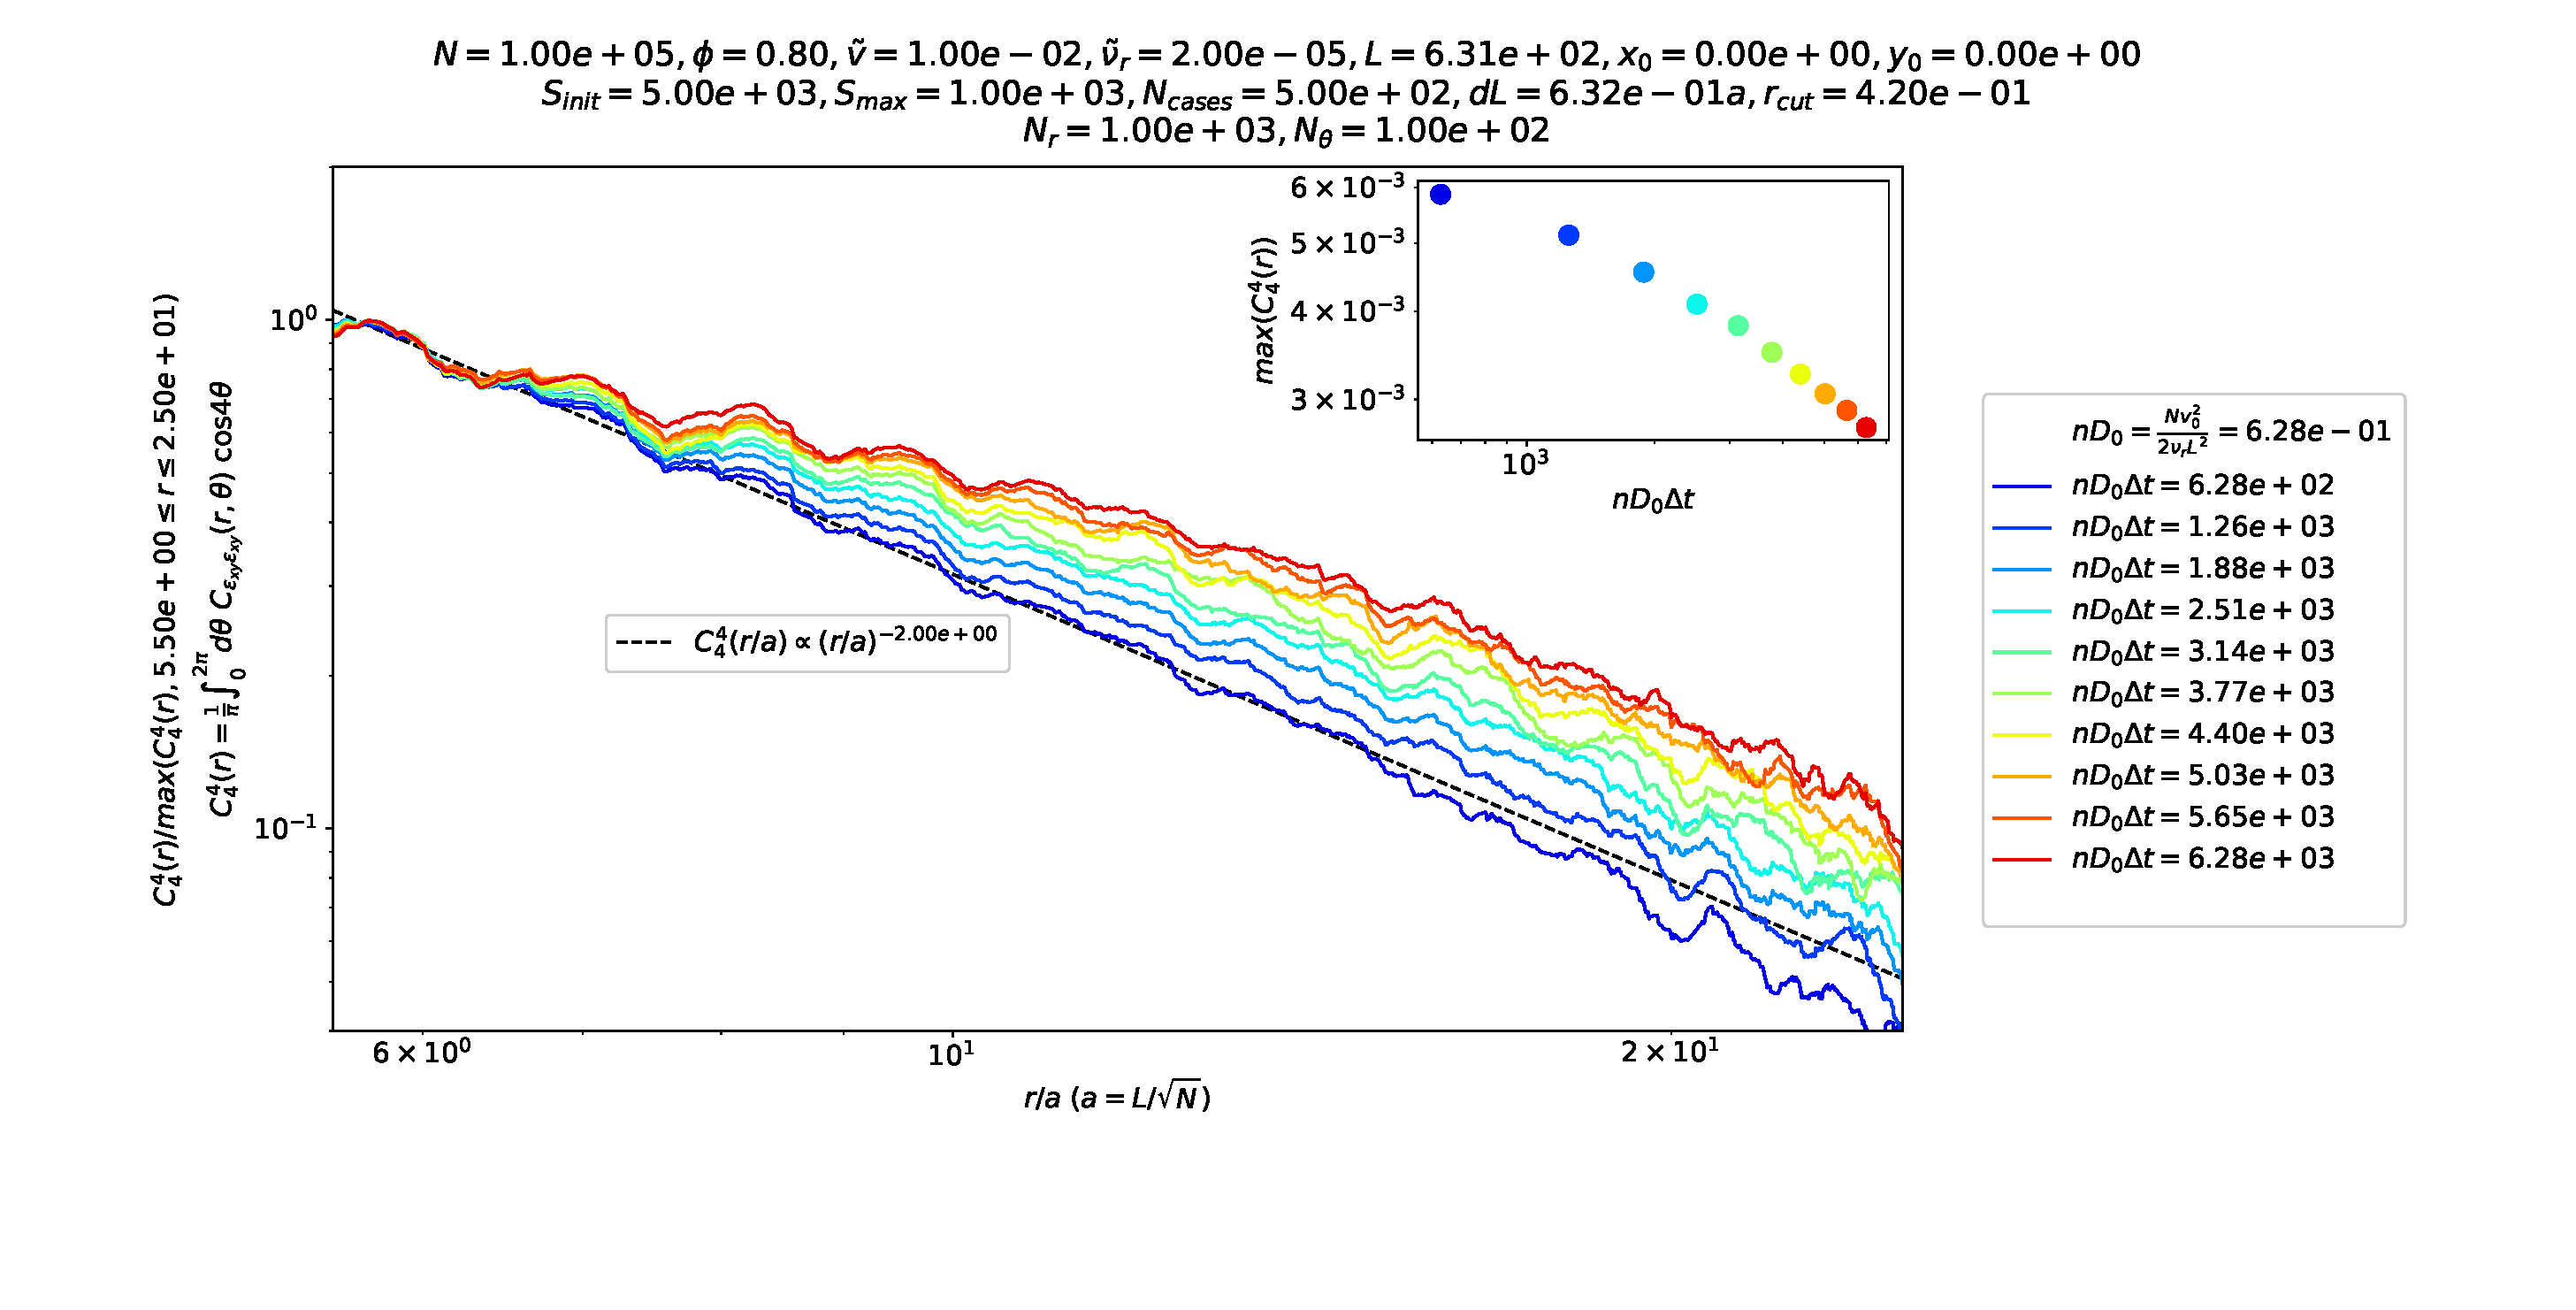
\includegraphics[width=\linewidth]{c44_max_cmsd_comparison_Dk8000_Vj1000_Rg2000_Nq1000_Ll0000_Mo1000_RCUTk4200_interpolated_loglog.eps}}
  \only<2>{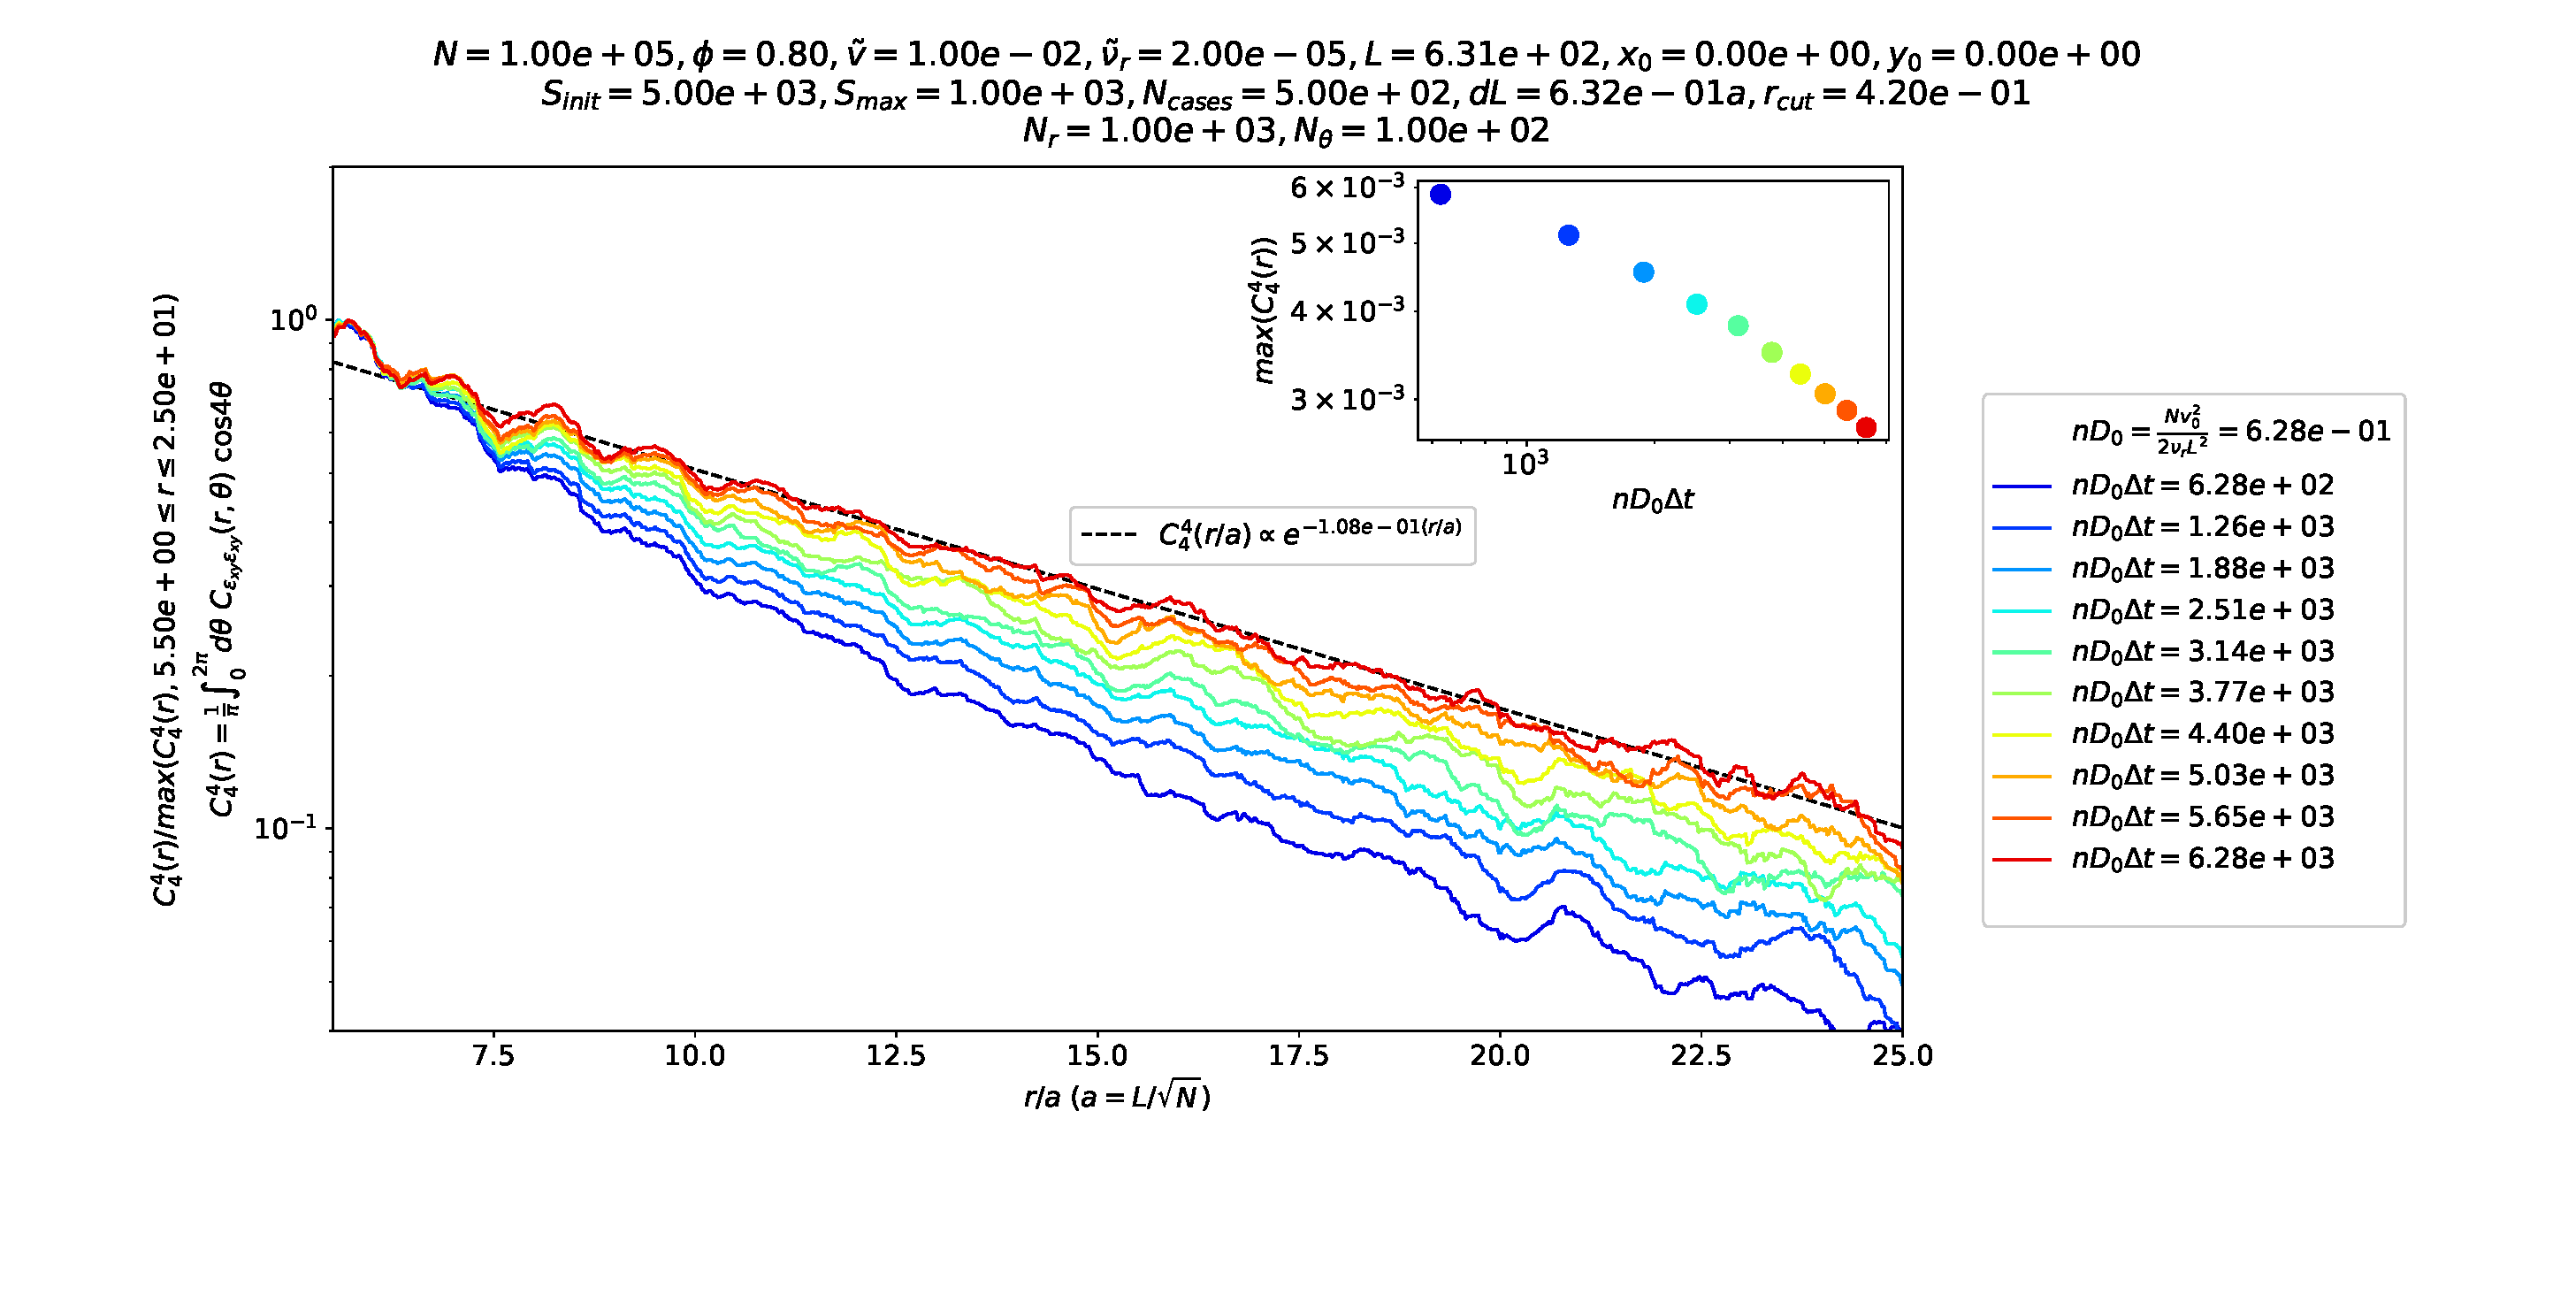
\includegraphics[width=\linewidth]{c44_max_cmsd_comparison_Dk8000_Vj1000_Rg2000_Nq1000_Ll0000_Mo1000_RCUTk4200_interpolated_linlog.eps}}
  \vspace{-0.8cm}
  \caption{Rescaled projections of shear strain correlations $C_4^4(\Delta r, \Delta t)$, at packing fraction $\phi=0.80$, self-propulsion velocity $\tilde{v}=1\cdot10^{-2}$ and rotation diffusion constant $\tilde{\nu}_r=2\cdot10^{-5}$.}
\end{figure}

\only<1>{\vspace{-0.8cm}}
\only<2>{\vspace{-0.5cm}}
\begin{itemize}
  \item[$\rightarrow$] \only<1>{Algebraic decay at low lag time with exponential cut-off.}\only<2>{Exponential decay at high lag time.}
\end{itemize}

\end{frame}

\begin{frame}{Projected strain correlations from CMSD at low activity}

\vspace{-0.4cm}
\begin{figure}[h!]
  \centering
  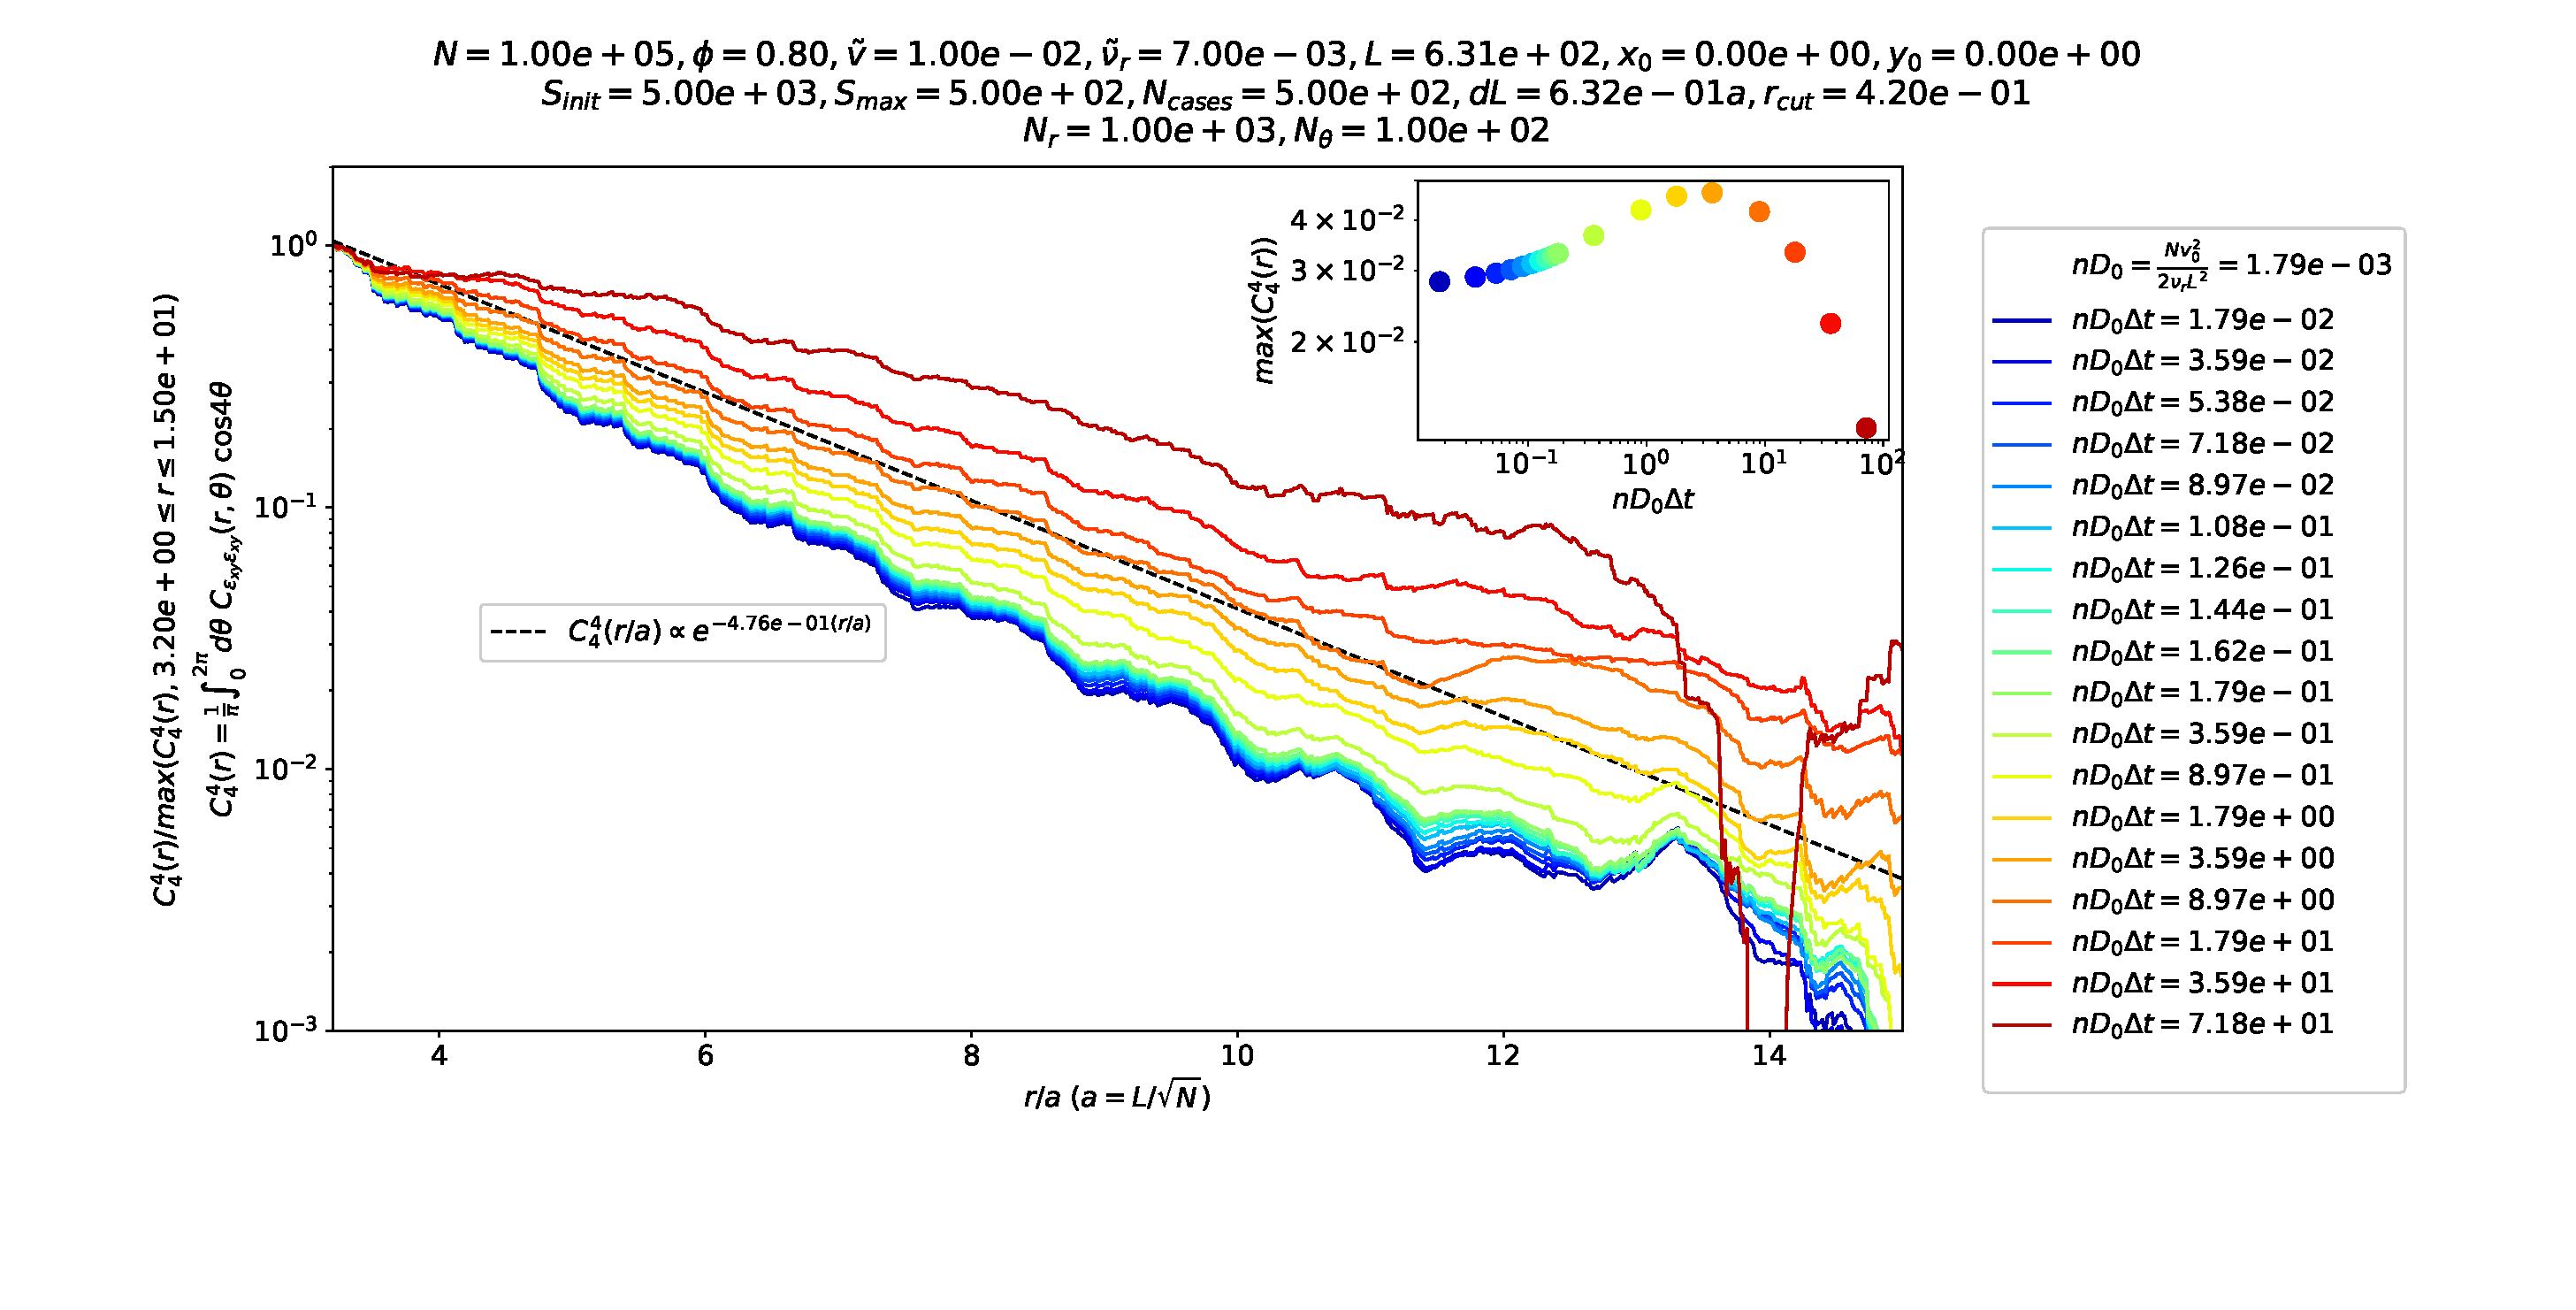
\includegraphics[width=0.95\linewidth]{c44_max_cmsd_comparison_Dk8000_Vj1000_Ri7000_Nq1000_Ll0000_RCUTk4200_interpolated_linlog.eps}
  \vspace{-0.8cm}
  \caption{Rescaled projections of shear strain correlations $C_4^4(\Delta r, \Delta t)$, at packing fraction $\phi=0.80$, self-propulsion velocity $\tilde{v}=1\cdot10^{-2}$ and rotation diffusion constant $\tilde{\nu}_r=7\cdot10^{-3}$.}
\end{figure}

\vspace{-0.8cm}
\begin{itemize}
  \item[$\rightarrow$] Exponential decay at all lag times.
  \item[$\rightarrow$] Exponential decay length scale around $2a$ and increasing function of lag time.
\end{itemize}

\end{frame}

\section{Conclusion}

\begin{frame}{Conclusion}

\begin{itemize}
\item Active matter system displaying motility-induced phase separation.
\only<2->{
\item At fixed self-propelling velocity, this transition is accompanied by increased cooperativity $\Rightarrow$ increased dynamical heterogeneity.
\item While at fixed rotation diffusion constant, it is accompanied by decreased cooperativity.
}
\only<3->{
\begin{itemize}
  \item[$\Rightarrow$] Péclet number is not enough to characterise the variations of the cooperativity and time of maximum cooperativity.
\end{itemize}
}
\only<4>{
\item Shear strain correlations show algebraic decay for phase-separated systems and exponential decay for homogenouis fluid systems.
}
\end{itemize}

\end{frame}

\begin{frame}{Outlook}

\begin{itemize}
\item Explore other paths through phase space to understand variations of cooperativities.
\only<2>{
\item Characterise the transition from exponential to algebraic decay in shear strain correlations.
}
\end{itemize}

\end{frame}

\end{document}
